%%  A simple AAU report template.

%
%  A simple AAU report template.
%  2014-09-13 v. 1.1.0
%  Copyright 2010-2014 by Jesper Kjær Nielsen <jkn@es.aau.dk>
%
%  This is free software: you can redistribute it and/or modify
%  it under the terms of the GNU General Public License as published by
%  the Free Software Foundation, either version 3 of the License, or
%  (at your option) any later version.
%
%  This is distributed in the hope that it will be useful,
%  but WITHOUT ANY WARRANTY; without even the implied warranty of
%  MERCHANTABILITY or FITNESS FOR A PARTICULAR PURPOSE.  See the
%  GNU General Public License for more details.
%
%  You can find the GNU General Public License at <http://www.gnu.org/licenses/>.
%
\documentclass[11pt,twoside,a4paper,openright]{report}
%%%%%%%%%%%%%%%%%%%%%%%%%%%%%%%%%%%%%%%%%%%%%%%%
% Language, Encoding and Fonts
% http://en.wikibooks.org/wiki/LaTeX/Internationalization
%%%%%%%%%%%%%%%%%%%%%%%%%%%%%%%%%%%%%%%%%%%%%%%%
% Select encoding of your inputs. Depends on
% your operating system and its default input
% encoding. Typically, you should use
%   Linux  : utf8 (most modern Linux distributions)
%            latin1 
%   Windows: ansinew
%            latin1 (works in most cases)
%   Mac    : applemac
% Notice that you can manually change the input
% encoding of your files by selecting "save as"
% an select the desired input encoding. 
\usepackage[utf8]{inputenc}
% Make latex understand and use the typographic
% rules of the language used in the document.
\usepackage[danish,english]{babel}
% Use the vector font Latin Modern which is going
% to be the default font in latex in the future.
\usepackage{lmodern}
% Choose the font encoding
\usepackage[T1]{fontenc}
% For checkmarks: \cmark and crossmarks: \xmark
\usepackage{pifont}
	\newcommand{\cmark}{\ding{51}}%
	\newcommand{\xmark}{\ding{55}}%
%%%%%%%%%%%%%%%%%%%%%%%%%%%%%%%%%%%%%%%%%%%%%%%%
% Graphics and Tables
% http://en.wikibooks.org/wiki/LaTeX/Importing_Graphics
% http://en.wikibooks.org/wiki/LaTeX/Tables
% http://en.wikibooks.org/wiki/LaTeX/Colors
%%%%%%%%%%%%%%%%%%%%%%%%%%%%%%%%%%%%%%%%%%%%%%%%
% load a colour package
\usepackage[table,dvipsnames]{xcolor}
\definecolor{aaublue}{RGB}{33,26,82}% dark blue
\definecolor{lightGrey}{RGB}{240,240,240}% 
% The standard graphics inclusion package
\usepackage{graphicx}
% Load package to convert eps-files to use as figures
\usepackage{epstopdf}

%\usepackage[dvips,final]{graphicx} 
%\usepackage[dvips]{geometry}
\usepackage{color} %include even if images aren’t in color \usepackage{epsfig}
\usepackage{latexsym}
\usepackage{pstricks}

%\usepackage{epsfig}

% Set up how figure and table captions are displayed
\usepackage{caption}
\captionsetup{%
  font=footnotesize,% set font size to footnotesize
  labelfont=bf % bold label (e.g., Figure 3.2) font
}
% For figures
\usepackage{float}
% For subfigures
\usepackage{subcaption}
% Make the standard latex tables look so much better
\usepackage{array,booktabs}
% Enable the use of frames around, e.g., theorems
% The framed package is used in the example environment
\usepackage{framed}
\usepackage{epstopdf}

% Afstand mellem listepunkter og tilføjelse af resume funktion til lister: \begin{enumerate}[resume]
\usepackage{enumitem}
\setlist{itemsep=-2pt}

% Tilføjer mulighed for at lave enkelte sider i landskab.
\usepackage{lscape}
\usepackage{rotating}

\newcounter{listcounter}
%%%%%%%%%%%%%%%%%%%%%%%%%%%%%%%%%%%%%%%%%%%%%%%%
% Mathematics
% http://en.wikibooks.org/wiki/LaTeX/Mathematics
%%%%%%%%%%%%%%%%%%%%%%%%%%%%%%%%%%%%%%%%%%%%%%%%
% Defines new environments such as equation,
% align and split 
\usepackage{amsmath}
% Adds new math symbols
\usepackage{amssymb}
% Use theorems in your document
% The ntheorem package is also used for the example environment
% When using thmmarks, amsmath must be an option as well. Otherwise \eqref doesn't work anymore.
\usepackage[framed,amsmath,thmmarks]{ntheorem}

% Tilføjer \degree symbol
\usepackage{textcomp}
\usepackage{gensymb}

% Fjerner mellemrum efter komma i formler.
%\usepackage{icomma}

% Packages for SI units
\usepackage[binary-units]{siunitx}
% Format SI units as italic in italic texts
\sisetup{detect-all}
\sisetup{per-mode=symbol}


% Argument til amsmath der gør parenteser uden om parenteser pænere ved brug af \right og \left kommandoerne
\delimitershortfall=-1pt

%%%%%%%%%%%%%%%%%%%%%%%%%%%%%%%%%%%%%%%%%%%%%%%%
% Page Layout
% http://en.wikibooks.org/wiki/LaTeX/Page_Layout
%%%%%%%%%%%%%%%%%%%%%%%%%%%%%%%%%%%%%%%%%%%%%%%%
% Change margins, papersize, etc of the document
\usepackage[
  inner=28mm,% left margin on an odd page
  outer=41mm,% right margin on an odd page
  ]{geometry}
% Modify how \chapter, \section, etc. look
% The titlesec package is very configureable
\usepackage[explicit]{titlesec}
%\titleformat*{\section}{\normalfont\Large\bfseries\color{aaublue}}
%\titleformat*{\subsection}{\normalfont\large\bfseries\color{aaublue}}
%\titleformat*{\subsubsection}{\normalfont\normalsize\bfseries\color{aaublue}}
%\titleformat*{\paragraph}{\normalfont\normalsize\bfseries\color{aaublue}}
%\titleformat*{\subparagraph}{\normalfont\normalsize\bfseries\color{aaublue}}
\usepackage{calc}

% Spacing omkring kapiteloverskrift
\titlespacing*{\chapter}{0pt}{40pt}{50pt}

% Overskrift med stort nummer til venstre og titel til højre
%\newlength\chapnumb
%\setlength{\chapnumb}{1.5cm}
%\titleformat{\chapter}[block]
%{\normalfont\bfseries}{}{0pt}
%{\parbox[b]{\chapnumb}{%
	  %\fontsize{2cm}{0}\selectfont\thechapter}%
  %\parbox[b]{\dimexpr\textwidth-\chapnumb\relax}{%
    %\raggedleft%
    %\hfill{\Huge#1}\\
    %\rule{\dimexpr\textwidth-\chapnumb\relax}{.5pt}}}
%\titleformat{name=\chapter,numberless}[block]
%{\normalfont\bfseries}{}{0pt}
	%{\Huge#1}

% Clear empty pages between chapters
\let\origdoublepage\cleardoublepage
\newcommand{\clearemptydoublepage}{%
  \clearpage
  {\pagestyle{empty}\origdoublepage}%
}
\let\cleardoublepage\clearemptydoublepage

% Change the headers and footers
\usepackage{fancyhdr}
\pagestyle{fancy}
\fancyhf{} %delete everything
\renewcommand{\headrulewidth}{0pt} %remove the horizontal line in the header
\fancyhead[RE]{\color{black}\small\nouppercase\leftmark} %even page - chapter title
\fancyhead[LO]{\color{black}\small\nouppercase\rightmark} %uneven page - section title
\fancyhead[LE,RO]{\thepage} %page number on all pages
% Do not stretch the content of a page. Instead,
% insert white space at the bottom of the page
\raggedbottom
% Enable arithmetics with length. Useful when
% typesetting the layout.

\setlength{\headheight}{14pt}

% Raise penalties for bastards
\widowpenalty=10000
\clubpenalty=10000

%%%%%%%%%%%%%%%%%%%%%%%%%%%%%%%%%%%%%%%%%%%%%%%%
% Table of Contents
% http://en.wikibooks.org/wiki/LaTeX/Bibliography_Management
%%%%%%%%%%%%%%%%%%%%%%%%%%%%%%%%%%%%%%%%%%%%%%%%
% Add additional commands for Table of Contents
\usepackage{bookmark}

{\setcounter{tocdepth}{1}}

% Control of space between items in Table of Contents
\usepackage[titles]{tocloft}
\setlength{\cftbeforepartskip}{10pt}
\setlength{\cftbeforechapskip}{4pt}
\setlength{\cftbeforesecskip}{2pt}
%%%%%%%%%%%%%%%%%%%%%%%%%%%%%%%%%%%%%%%%%%%%%%%%
% Bibliography
% http://en.wikibooks.org/wiki/LaTeX/Bibliography_Management
%%%%%%%%%%%%%%%%%%%%%%%%%%%%%%%%%%%%%%%%%%%%%%%%
% Add the \citep{key} command which display a
% reference as [author, year]
\usepackage[square]{natbib}

%%%%%%%%%%%%%%%%%%%%%%%%%%%%%%%%%%%%%%%%%%%%%%%%
% Misc
%%%%%%%%%%%%%%%%%%%%%%%%%%%%%%%%%%%%%%%%%%%%%%%%
% Add bibliography and index to the table of
% contents
\usepackage[nottoc]{tocbibind}
% Add the command \pageref{LastPage} which refers to the
% page number of the last page
\usepackage{lastpage}
\usepackage[
%  disable, %turn off todonotes
  colorinlistoftodos, %enable a coloured square in the list of todos
  textwidth=\marginparwidth, %set the width of the todonotes
  textsize=scriptsize, %size of the text in the todonotes
  ]{todonotes}

% Add command \includepdf to add a whole pdf page to document
\usepackage{pdfpages}


% Add option to easy format directory tree
\usepackage{dirtree}

% String manipulation
\usepackage{xstring,xifthen}

% Tikz package for drawing nice figures
\usepackage{tikz}

% Package for drawing pretty schematics, without leaving LaTex
\usepackage[american currents, american voltages, european resistors, cute inductors,
american ports]{circuitikz}

% Code syntax highlight
\usepackage{listings}
\lstset{breaklines=true,
		breakatwhitespace=true,
		commentstyle=\color{ForestGreen},
		numbers=left,
		numberstyle=\tiny\color{black},
		keywordstyle=\color{blue},
		basicstyle=\footnotesize\ttfamily,
        showstringspaces=false,
		}
\renewcommand{\lstlistingname}{Code Snippet}

%%%%%%%%%%%%%%%%%%%%%%%%%%%%%%%%%%%%%%%%%%%%%%%%
% Table environments
% http://en.wikibooks.org/wiki/LaTeX/Tables
%%%%%%%%%%%%%%%%%%%%%%%%%%%%%%%%%%%%%%%%%%%%%%%%
% Better table environments for stuff like table width specifier
\usepackage{tabularx}
\usepackage{multirow}
\usepackage{longtable}
%%%%%%%%%%%%%%%%%%%%%%%%%%%%%%%%%%%%%%%%%%%%%%%%
% Project info and abstract
% chapters\abstract.tex, chapters\projectinfo.tex
%%%%%%%%%%%%%%%%%%%%%%%%%%%%%%%%%%%%%%%%%%%%%%%%
% Loads project info and abstract for use in
% hypersetup
\newcommand{\projectFaculty}{%
\iflanguage{english}{%
Electronic Engineering and IT%
}{%
Elektronik og IT%
}}

\newcommand{\projectGroup}{%
\iflanguage{english}{%
SPA10-1076%
}{%
Gruppe %
}}

\newcommand{\projectSemester}{%
P10%
}

\newcommand{\projectType}{%
\iflanguage{english}{%
Master Thesis%
}{%
Projektrapport%
}}

\newcommand{\projectTitle}{%
\iflanguage{english}{%
Sound control in windy weather%
}{%
Intelligibility of air and bone conducted speech in noise%
}}

\newcommand{\projectSubtitle}{%
\iflanguage{english}{%
- Subtitle -%
}{%
- Undertitel -%
}}

\newcommand{\projectTheme}{%
\iflanguage{english}{%
Signal Processing and Acoustics 
}{%
Digitale og analoge systemer i samspil med omverdenen%
}}

\newcommand{\projectPeriod}{%
\iflanguage{english}{%
MSc, 10th Semester 2019%
}{%
Efterårssemester 2016%
}}



\newcommand{\projectParticipants}{%
Jonas Buchholdt\\
}

\newcommand{\projectSupervisors}{%
Sofus Birkedal Nielsen
}

\newcommand{\projectCopies}{8}

\newcommand{\projectCompletion}{
\iflanguage{english}{%
6\textsuperscript{th} June 2019
}{
30\textsuperscript{th} may 2019%
}}




\newcommand{\projectAbstract}{
%The paper deals with the creation of different sound effects for an electric guitar on the a Digital Signal Processor. Some of these effects are the reverb, the flanger and the equalizer. 
%The report includes a thorough explanation of each of the effects followed by the used design approach. Simulations on MATLAB were done to verify the design. All the effects have been coded in assembly for the DSP implementation.  The Assembly code works with the TMS320C5515 DSP from Texas Instruments. 
%In order to make the DSP usable on a variety of electric guitars, a preamplifier was built. All details relating to the design and the implementation of this component are included in the paper as well. 


%The scope of the project at hand is investigating the speech intelligibility, that is achieve via bone-conducted (BC) sound compared to that of airbone sound.
%After extensive literature research, a perceptual is designed. A loudness matching routine is developed, speech intelligibility is tested with a procedure, that is a modified version of the Danish Hearing In Noise Test (HINT). The Bone-conduction Intelligibility Evaluation Routine (BIER) is executed with ten normal hearing subjects. The analysis of the results hints towards a worse conduction of the bone conduction tranducer in terms of intelligibility, that cannot be shown to be statistically significant.


%This project deals with low/mid frequency directivity control.
%The directional characteristics of a single loudspeaker and position of its acoustic center are characterised. An analytical model of the loudspeaker is established to model a beamforming array. After pointing out some properties of the commonly known first order gradient source, a three speaker array is designed. Three speakers are chosen to overcome the disadvantage of the first order gradient speaker not being able to freely control its main lobe direction. To predict the behaviour of the speaker array in a non-free-field environment, a numerical model is set up.  A genetic algorithm is chosen to optimize gain and phase for the individual loudspeakers. A suitable positioning scheme for the speakers is established. Required signal processing parameters are implemented as filters. The measured directional characteristics of the array are compared with the analytical and numerical models and compared with the directional characteristics of a commercial product.

The scope of this thesis is to investigate the effect of inhomogeneous atmospheric condition on sound propagation from a line source array. It is founded in the analysis that the wind refracts the sound wave and the \gls{spl} coverage of the line source array is uneven. A solution is proposed to minimise the  \gls{spl} coverage differences in the line source coverage area. The solution deals with both crosswind and parallel wind. In the parallel wind case, only upwards refraction is analysed. Measurement shows that the \gls{spl} coverage can be optimised from a difference of over \dBr{17} to less than \dBr{3} between the upwards and downwards direction. Moreover, the \gls{spl} in the shadow zone is raised in parallel wind condition by forward tilting of the line source array.  

}

\newcommand{\projectSynopsis}{
Synopsis
}

%%%%%%%%%%%%%%%%%%%%%%%%%%%%%%%%%%%%%%%%%%%%%%%%
% Hyperlinks
% http://en.wikibooks.org/wiki/LaTeX/Hyperlinks
%%%%%%%%%%%%%%%%%%%%%%%%%%%%%%%%%%%%%%%%%%%%%%%%
% Enable hyperlinks and insert info into the pdf
% file. Hypperref should be loaded as one of the 
% last packages
\usepackage{hyperref}
\hypersetup{%
	%pdfpagelabels=true,%
	plainpages=false,%
	pdfauthor={\projectGroup, \projectFaculty, \iflanguage{english}{Aalborg University}{Aalborg Universitet}},%
	pdftitle={\projectTitle},%
	pdfsubject={\projectTheme},%
	bookmarksnumbered=true,%
	colorlinks,%
	citecolor=black,%aaublue,%
	filecolor=black,%aaublue,%
	linkcolor=black,%aaublue,% you should probably change this to black before printing
	urlcolor=black,%aaublue,%
	pdfstartview=FitH,%
	bookmarksdepth=2,%
}

% Defines where URLs should break
\def\UrlBreaks{\do\/\do-\do_}
\urlstyle{same}

% Give the possibility to autoformat reference based on distance to the referenced page. Ex. \vpageref{}
\usepackage{varioref}


% Package to warn about missing references.
%\usepackage{refcheck}

% Package to make a glossary of acronyms.
\usepackage{glossaries}
\glstoctrue
\makenoidxglossaries
% Glossaries package
% http://ctan.cs.uu.nl/macros/latex/contrib/glossaries/glossariesbegin.pdf
%
% % % % % % % %
%	Example of glossary entry:
% \newglossaryentry{cabbage}{name={cabbage},description={vegetable with thick green or purple leaves}}
%
%	Example of acronym entry:
% \newacronym{spi}{SPI}{Serial Peripheral Interface}
%


\newacronym{dgps}{DGPS}{Differential \glsentryshort{gps}}
\newacronym{spl}{SPL}{Sound Pressure Level}
\newacronym{db}{dB}{Decibel}
\newacronym{hz}{Hz}{Hertz}
\newacronym{ft}{FT}{Fourier Transform}
\newacronym{ift}{IFT}{Inverse Fourier Transform}
\newacronym{fft}{FFT}{Fast Fourier Transform}
\newacronym{ifft}{IFFT}{Inverse Fast Fourier Transform}
\newacronym{ttl}{TTL}{Transistor–Transistor Logic}
\newacronym{dll}{DLL}{Dynamic Link library}
\newacronym{udp}{UDP}{User Datagram Protocol}
\newacronym{ip}{IP}{Internet Protocol}
 \newacronym{dut}{DUT}{Device Under Test}
 \newacronym{usb}{USB}{Universal Serial Bus} 
\newacronym{bandk}{B\&K}{Brüel \& Kjær}
\newacronym{mdf}{MDF}{medium-density fibreboard}
\newacronym{rms}{RMS}{Root Mean Square}
\newacronym{fdtd}{FDTD}{Finite-Difference Time-Domain}
\newacronym{sp}{SP}{Signal Processing}
\newacronym{ga}{GA}{Genetic Algorithm}
\newacronym{dc}{DC}{Direct Current}
\newacronym{fir}{FIR}{Finite Impulse Response}
\newacronym{iir}{IIR}{Infinite Impulse Response}
\newacronym{aau}{AAU}{Aalborg University}
\newacronym{bc}{BC}{Bone Conduction}
\newacronym{bct}{BCT}{Bone Conduction Transducer}
\newacronym{ac}{AC}{Air Conduction}
\newacronym{acs}{ACS}{Air Conduction Speaker}
\newacronym{ace}{ACE}{Air Conduction Earphones}
\newacronym{hrtf}{HRTF}{Head Related Transfer Function}
\newacronym{bm}{BM}{Basilar Membrane}
\newacronym{best}{BEST}{Balanced Electromagnetic Separation Transducer}
\newacronym{csf}{CSF}{Cerebrospinal Fluid}
\newacronym{sti}{STI}{Speech Transmission Index}
\newacronym{pa}{PA}{Public Address}
\newacronym{cat}{CAT}{Callsign Acquisition Test}
\newacronym{hint}{HINT}{Hearing in Noise Test}
\newacronym{fst}{FST}{Freiburger Sprachtest}
\newacronym{mrt}{MRT}{Modified Rhyme Test}
\newacronym{fmcbct}{FMCBCT}{Free-field Method to Calibrate Bone Conduction Transducers}
\newacronym{bier}{BIER}{Bone-conducted Intelligibility Evaluation Routine}
\newacronym{pdf}{PDF}{Probability Density Function}
\newacronym{snr}{SNR}{Signal to Noise Ratio}
\newacronym{srtn}{SRT\textsubscript{N}}{Speech Recognition Threshold in Noise}
\newacronym{mse}{MSE}{Mean Square Error}
\newacronym{acv}{ACV}{Alternating Current Voltage}
\newacronym{srt}{SRT}{Speech Recognition Threshold}
\newacronym{cdf}{CDF}{Cumulative Distribution Function}
\newacronym{ssn}{SSN}{Speech Shaped Noise}
\newacronym{acalos}{ACALOS}{Adaptive Categorical Loudness Scaling}
\newacronym{hl}{HL}{Hearing threshold Level}
\newacronym{clue}{CLUE}{Conversational Language Understanding Evaluation}
\newacronym{foh}{FOH}{Front Of House}
\newacronym{dsp}{DSP}{Digital Signal Processor}
\newacronym{fifo}{FIFO}{First In First Out}
\newacronym{adc}{ADC}{Analog to Digital Converter}
\newacronym{pcb}{PCB}{Printed Circuit Board}


% Package to make semi-bold font.
\usepackage[outline]{contour}
\contourlength{0.1pt}
\contournumber{50}%
\newcommand{\textsb}[1]{\contour{black}{#1}}

% Package for splitting lists or other things up in columns. Ex: \begin{multicols}{2}
\usepackage{multicol}

% Package for rotating a page to landscape orientation. Ex: \begin{landscape}
\usepackage{pdflscape}

% For adding notes to tables
\usepackage{threeparttable}

% For adding smileys ;) I know....
\usepackage{MnSymbol,wasysym}

% For adding algorithms
\usepackage{algorithm}
\usepackage[noend]{algpseudocode}
\makeatletter
\def\BState{\State\hskip-\ALG@thistlm}
\makeatother

\renewcommand*{\glsgroupskip}{\vspace{2mm}}
% ps to PDF


%Highlight
\usepackage{soul}
\usepackage{amsmath}


\usepackage{pdfpages}
\usepackage{csquotes}

\usepackage{tabularx}
\def\arraystretch{1.5}%
\renewcommand{\arraystretch}{1.5}

\usepackage{graphicx}
\usepackage{pgfplots}
\usepackage{nicefrac}
\usepackage{xfrac}
\usepackage{pgf}
\usepackage{fp,xstring}
%\usepackage{floatrow}
%\usepackage{ebgaramond}
\usepackage{graphicx, caption} %






%\usepackage{heuristica}
%\usepackage[textwidth =15cm]{geometry}

%\usepackage{graphicx}
%\usepackage{caption, threeparttable}
%\captionsetup{labelfont = sc, textfont = it}


% tikz colour %
\definecolor{mycolor1}{rgb}{0.00000,0.44700,0.74100}  % the good blue
\definecolor{mycolor2}{rgb}{0.85000,0.32500,0.09800}  % the orange
\definecolor{mycolor3}{rgb}{0.00,0.39,0.00}  % the dark green
\definecolor{mycolor4}{rgb}{0.40,0.00,0.60} % concord grape violet
\definecolor{mycolor5}{rgb}{0.80,0.80,0.08} % the yellow
\definecolor{mycolor6}{rgb}{0.37,0.15,0.07} % the brown


%Measurememt gloss


%\usepackage[acronym]{glossaries}
%\renewcommand*{\acronymname}{Measurement}
%\newglossary[tlg]{domain}{tld}{tdn}{Top-Level Domains}

\usepgfplotslibrary{external} 
\usetikzlibrary{external}
\tikzexternalize[prefix=tikz/]
\pgfplotsset{compat=1.13}
\usetikzlibrary{plotmarks}



\newcommand\Tstrut{\rule{0pt}{2.6ex}}       % "top" strut
\newcommand\Bstrut{\rule[-0.9ex]{0pt}{0pt}} % "bottom" strut
\newcommand{\TBstrut}{\Tstrut\Bstrut} % top&bottom struts% Package inclusion and set up of the document

% see, e.g., http://en.wikibooks.org/wiki/LaTeX/Formatting#Hyphenation
% for more information on word hyphenation
\hyphenation{ex-am-ple hy-phen-a-tion short}
\hyphenation{long la-tex}
\hyphenation{AAU-Sat}
\hyphenation{minimum-spændinger}
\hyphenation{ud-vik-lings-poten-tiale}
\hyphenation{pick-up pick-up-pen gui-tar-pick-up gui-tar-pick-up-pen pick-uppens}
\hyphenation{tech-no-lo-gy}
\hyphenation{Hø-re-for-e-ning-en}% Hypenation setup



%%%%%%%%%%%%%%%%%%%%%%%%%%%%%%%%%%%%%%%%%%%%%%%%
% Loads user defined variables
%%%%%%%%%%%%%%%%%%%%%%%%%%%%%%%%%%%%%%%%%%%%%%%%

\newcommand{\noSIunit}{$1$}% Definerer hvad der skal skrives hvis symbolet ikke har nogen enhed.
\newcommand{\obcTransducerAddress}{0xB1}% CAN adresse til tranducer modulet i OBC.

\def\circuitScale{.5}%

%%%%%%%%%%%%%%%%%%%%%%%%%%%%%%%%%%%%%%%%%%%%%%%%
% Macros for the titlepage
%%%%%%%%%%%%%%%%%%%%%%%%%%%%%%%%%%%%%%%%%%%%%%%%
%Creates the aau titlepage
\newcommand{\aautitlepage}[3]{%
  {
    %set up various length
    \ifx\titlepageleftcolumnwidth\undefined
      \newlength{\titlepageleftcolumnwidth}
      \newlength{\titlepagerightcolumnwidth}
    \fi
    \setlength{\titlepageleftcolumnwidth}{0.5\textwidth-\tabcolsep}
    \setlength{\titlepagerightcolumnwidth}{\textwidth-2\tabcolsep-\titlepageleftcolumnwidth}
    %create title page
    \thispagestyle{empty}
    \noindent%
    \begin{tabular}{@{}ll@{}}
      \parbox{\titlepageleftcolumnwidth}{
        \iflanguage{danish}{%
          
\includegraphics[page=1,width=\titlepageleftcolumnwidth]{figures/aau_logo}
        }{%
          
\includegraphics[page=2,width=\titlepageleftcolumnwidth]{figures/aau_logo}
        }
      } &
      \parbox{\titlepagerightcolumnwidth}{\raggedleft\sf\small
        #2
      }\bigskip\\
       #1 &
      \parbox[t]{\titlepagerightcolumnwidth}{%
        \iflanguage{danish}{%
          \textbf{Synopsis:}\smallskip\par
        }{%
          \textbf{Abstract:}\smallskip\par
        }
        \fbox{\parbox{\titlepagerightcolumnwidth-2\fboxsep-2\fboxrule}{%
          #3
        }}
      }\\
    \end{tabular}
    \vfill
    \iflanguage{danish}{%
      \noindent{\footnotesize\emph{Rapportens indhold er frit tilgængeligt, men offentliggørelse (med kildeangivelse) må kun ske efter aftale med forfatterne.}}
    }{%
      \noindent{\footnotesize\emph{The content of this report is freely available, but publication may only be pursued with reference.}}
    }
    \cleardoublepage
  }
}

%Create english project info
\newcommand{\englishprojectinfo}[8]{%
  \parbox[t]{\titlepageleftcolumnwidth}{
    \textbf{Title:}\\ #1\bigskip\par
    \textbf{Theme:}\\ #2\bigskip\par
    \textbf{Project Period:}\\ #3\bigskip\par
    \textbf{Project Group:}\\ #4\bigskip\par
    \textbf{Participants:}\\ #5\bigskip\par
    \textbf{Supervisor:}\\ #6\bigskip\par
    \textbf{Number of Pages:} \pageref{LastPage}\bigskip\par
    \textbf{Date of Completion:}\\ #8
  }
}

%Create danish project info
\newcommand{\danishprojectinfo}[8]{%
  \parbox[t]{\titlepageleftcolumnwidth}{
    \textbf{Titel:}\\ #1\bigskip\par
    \textbf{Tema:}\\ #2\bigskip\par
    \textbf{Projektperiode:}\\ #3\bigskip\par
    \textbf{Projektgruppe:}\\ #4\bigskip\par
    \textbf{Deltagere:}\\ #5\bigskip\par
    \textbf{Vejleder:}\\ #6\bigskip\par
    \textbf{Oplagstal:} #7\bigskip\par
    \textbf{Sidetal:} \pageref{LastPage}\bigskip\par
    \textbf{Afleveringsdato:}\\ #8
  }
}

%%%%%%%%%%%%%%%%%%%%%%%%%%%%%%%%%%%%%%%%%%%%%%%%
% An example environment
%%%%%%%%%%%%%%%%%%%%%%%%%%%%%%%%%%%%%%%%%%%%%%%%
\theoremheaderfont{\normalfont\bfseries}
\theorembodyfont{\normalfont}
\theoremstyle{break}
\def\theoremframecommand{{\color{aaublue!50}\vrule width 5pt \hspace{5pt}}}
\newshadedtheorem{exa}{Example}[chapter]
\newenvironment{example}[1]{%
		\begin{exa}[#1]
}{%
		\end{exa}
}


%%%%%%%%%%%%%%%%%%%%%%%%%%%%%%%%%%%%%%%%%%%%%%%%%
% Exponential function defined as upright e, \exp
%%%%%%%%%%%%%%%%%%%%%%%%%%%%%%%%%%%%%%%%%%%%%%%%%
\renewcommand{\exp}{\text{e}}


%%%%%%%%%%%%%%%%%%%%%%%%%%%%%%%%%%%%%%%%%%%%%%%%%%%
% Command \clearevenpage start chapter on even page
%%%%%%%%%%%%%%%%%%%%%%%%%%%%%%%%%%%%%%%%%%%%%%%%%%%
\makeatletter
\newcommand*{\clearevenpage}{%
  \clearpage
  \if@twoside
    \ifodd\c@page
      \hbox{}%
      \newpage
      \if@twocolumn
        \hbox{}%
        \newpage
      \fi
    \fi
  \fi
}
\makeatother

%%%%%%%%%%%%%%%%%%%%%%%%%%%%%%%%%%%%%%%%%%%%%%%%%%%%%%%
% Command \addunit. Use it to add si units to equations
%%%%%%%%%%%%%%%%%%%%%%%%%%%%%%%%%%%%%%%%%%%%%%%%%%%%%%%
\makeatletter
\providecommand\add@text{}
\newcommand\addunit[1]{%
  \gdef\add@text{\text{[}\ifthenelse{\equal{#1}{}}{\noSIunit}{\si{#1}}\text{]}\gdef\add@text{}}}% 
\renewcommand\tagform@[1]{%
  \maketag@@@{\llap{\add@text\quad}(\ignorespaces#1\unskip\@@italiccorr)}%
}
\makeatother

%%%%%%%%%%%%%%%%%%%%%%%%%%%%%%%%%%%%%%%%%%%%%
% Oversættelser af ord ved brug af \autoref{}
%%%%%%%%%%%%%%%%%%%%%%%%%%%%%%%%%%%%%%%%%%%%%
\addto\extrasdanish{%
  \def\figureautorefname{Figur}%
  \def\subfigureautorefname{Figur}%
  \def\tableautorefname{Tabel}%
  \def\partautorefname{Del}%
  \def\appendixautorefname{Bilag}%
  \def\equationautorefname{Ligning}%
  \def\Itemautorefname{Punkt}%
  \def\chapterautorefname{Kapitel}%
  \def\sectionautorefname{Afsnit}%
  \def\subsectionautorefname{Afsnit}%
  \def\subsubsectionautorefname{Underafsnit}%
  \def\paragraphautorefname{Delafsnit}%
  \def\Hfootnoteautorefname{Fodnote}%
  \def\AMSautorefname{Ligning}%
  \def\theoremautorefname{Sætning}%
  \def\pageautorefname{Side}%
  \def\requirementautorefname{Krav}%
}

\addto\extrasenglish{%
  \def\sectionautorefname{section}%
  \def\subsectionautorefname{section}%
  \def\subsubsectionautorefname{section}%
  \def\requirementautorefname{Requirement}%
  \def\algorithmautorefname{Algorithm}%
}

%%%%%%%%%%%%%%%%%%%%%%%%%%%%%%%%%%%%%%%%%%%%%%%%%%%%%%%%%%%%%%%%%%%%%%
% Tilføjer kommando \fullref{} for både at referere til nummer og navn
%%%%%%%%%%%%%%%%%%%%%%%%%%%%%%%%%%%%%%%%%%%%%%%%%%%%%%%%%%%%%%%%%%%%%%
\renewcommand*{\fullref}[1]{\hyperref[{#1}]{\autoref*{#1} \nameref*{#1}}} % One single link


%%%%%%%%%%%%%%%%%%%%%%%%%%%%%%%%%%%%%%%%%%%%%%%%%%%%%%%%%%%%%%%%%%%%%%
% Tilføjer forkortelser af ord.
%%%%%%%%%%%%%%%%%%%%%%%%%%%%%%%%%%%%%%%%%%%%%%%%%%%%%%%%%%%%%%%%%%%%%%
\newcommand{\AAU}{%
\iflanguage{english}{%
Aalborg University%
}{%
Aalborg Universitet%
}}

\newcommand{\opamp}{%
\iflanguage{english}{%
operational amplifier%
}{%
operationsforstærker%
}}

\newcommand{\hifi}{%
\iflanguage{english}{%
hi-fi amplifier%
}{%
hi-fi-forstærker%
}}

%%%%%%%%%%%%%%%%%%%%%%%%%%%%%%%%%%%%%%%%%%%%%%%%%%%%%%%%%%%%%%%%%%%%%%
% Command \DefVar{VARIBLE_NAME}
% Is used to create a variable.
% Set varible: \VARIBLE_NAME{VALUE}
% Get varible: \getVARIBLE_NAME
%%%%%%%%%%%%%%%%%%%%%%%%%%%%%%%%%%%%%%%%%%%%%%%%%%%%%%%%%%%%%%%%%%%%%%

\makeatletter%
\newcommand{\DefVar}[1]{\@namedef{#1}##1{\global\@namedef{get#1}{##1}}\@nameuse{#1}{}}%
\makeatother%

%%%%%%%%%%%%%%%%%%%%%%%%%%%%%%%%%%%%%%%%%%%%%%%%%%%%%%%%%%%%%%%%%%%%%%
% Requirements environment:
%
% \begin{requirement}
%   \requirement{}
%   \argument{}
%   \fullfilment{}
% \end{requirement}
%%%%%%%%%%%%%%%%%%%%%%%%%%%%%%%%%%%%%%%%%%%%%%%%%%%%%%%%%%%%%%%%%%%%%%

\def\reqPrefixName{??}% Individual prefix for the requirements
\newcounter{reqIDCounter}% Requirement counter for the subsections
\newcounter{requirement}% Absolute requirement counter. Used to trigger label/reference target.

\newlength{\reqBoxWidth}% Create length varible to define width of requirement box
\setlength{\reqBoxWidth}{5cm}% Actual width of requirement box

\newcommand{\reqPrefix}[1]{% Command to define requirement prefix
\ifthenelse{\equal{#1}{}}{\reqPrefixName}{\setcounter{reqIDCounter}{0}\def\reqPrefixName{#1}}%
}

\makeatletter% Define requirementID for references
\newcommand{\reqLabel}{%
\protected@edef\@currentlabel{\reqPrefixName\thereqIDCounter}%
\protected@edef\@currentlabelname{Requirement}%
}\makeatother%

\newenvironment{requirement}%
{\par\vspace{\baselineskip}\noindent\ignorespaces%
\refstepcounter{requirement}%
\stepcounter{reqIDCounter}%
\reqLabel%
\DefVar{requirement}\DefVar{argument}%\DefVar{fullfilment}%
%
\tabularx{1\textwidth}{p{\reqBoxWidth} !{\color{white}{\vrule width 2pt}} X}%
\greyrow \parbox[t]{\reqBoxWidth}{\textsb{Update}\\\getrequirement\vskip1mm}% ~\reqPrefixName\thereqIDCounter
&%
\parbox[t]{\textwidth-\reqBoxWidth-4\tabcolsep-2pt}{\textsb{Argumentation}\\\getargument\vskip1mm}
%\addlinespace[2pt]%
%\greyrow \multicolumn{2}{l}{\parbox{\textwidth-2\tabcolsep}{\vskip1mm\textsb{Conditions of fulfilment}\\\getfullfilment\vskip1mm}}%
}%
{\endtabularx\par\ignorespacesafterend}


%%%%%%%%%%%%%%%%%%%%%%%%%%%%%%%%%%%%%%%%%%%%%%%%%%%%%%%%%%%%%%%%%%%%%%
% Tilføjer kommando \numnameref{labelnavn}
% Kommandoen tilføjer en reference til et afsnit med både nummer og navn.
%%%%%%%%%%%%%%%%%%%%%%%%%%%%%%%%%%%%%%%%%%%%%%%%%%%%%%%%%%%%%%%%%%%%%%
\newcommand{\numnameref}[1]{%
\hyperref[#1]{\autoref{#1}: \nameref{#1}}%
}

%%%%%%%%%%%%%%%%%%%%%%%%%%%%%%%%%%%%%%%%%%%%%%%%%%%%%%%%%%%%%%%%%%%%%%
% Defines subscript as upright text if it contains more than one character.
% 
%%%%%%%%%%%%%%%%%%%%%%%%%%%%%%%%%%%%%%%%%%%%%%%%%%%%%%%%%%%%%%%%%%%%%%

\catcode`\_=12% Makes underscore an inactive character
\begingroup\lccode`~=`\_% Loads underscore character for redefinition
\lowercase{\endgroup\def~}#1{% Start definition of underscore
\StrLen{#1}[\subscriptstringlen]% Determine length of subscript string
\ifthenelse{\subscriptstringlen=1}% Test if subscript string contain one character
{\sb{#1}}% Prints subscript as italic if only one character is present
{\sb{\mathrm{#1}}}}% Prints subscript as upright text if there are more than one character
\AtBeginDocument{\mathcode`\_=\string"8000 }% Makes underscore active only in math mode


%%%%%%%%%%%%%%%%%%%%%%%%%%%%%%%%%%%%%%%%%%%%%%%%%%%%%%%%%%%%%%%%%%%%%%
% Defind counter
% Bruges til forklaringer af ligninger og equpment
%%%%%%%%%%%%%%%%%%%%%%%%%%%%%%%%%%%%%%%%%%%%%%%%%%%%%%%%%%%%%%%%%%%%%%
\newcounter{firstexplain}% Holder styr på om det er den første symbolforklaring

%%%%%%%%%%%%%%%%%%%%%%%%%%%%%%%%%%%%%%%%%%%%%%%%%%%%%%%%%%%%%%%%%%%%%%
% Defind counter
% Bruges til forklaringer af ligninger og equpment
%%%%%%%%%%%%%%%%%%%%%%%%%%%%%%%%%%%%%%%%%%%%%%%%%%%%%%%%%%%%%%%%%%%%%%

%%%%%%%%%%%%%%%%%%%%%%%%%%%%%%%%%%%%%%%%%%%%%%%%%%%%%%%%%%%%%%%%%%%%%%
% Tilføjer kommando \startexplain, \stopexplain og \explain{variable}{test}{is unit}
% Bruges til forklaringer af ligninger.
%%%%%%%%%%%%%%%%%%%%%%%%%%%%%%%%%%%%%%%%%%%%%%%%%%%%%%%%%%%%%%%%%%%%%%
%\newcounter{firstexplain}% Holder styr på om det er den første symbolforklaring
%
%\def\startexplain{%
%	\setcounter{firstexplain}{1}%
%	{\noindent}%
%	{\par\noindent}
%	\begin{tabular}{@{}p{.06\columnwidth}p{.76\columnwidth}@{\hskip.04\columnwidth}p{.02\columnwidth}@{}}}%
%\def\stopexplain{\end{tabular}\\[10pt]}%
%
%\newcommand{\explain}[2]{%
%	\ifthenelse{\thefirstexplain=1}{%
%	Where:\\
%	&#1&[\ifthenelse{\equal{#2}{}}{\noSIunit}{#2}]\\\setcounter{firstexplain}{0}
%	}{%
%	&#1&[\ifthenelse{\equal{#2}{}}{\noSIunit}{#2}]\\%
%	}%
%}%




\def\startexplain{\setcounter{firstexplain}{1}{\noindent}{\par\noindent}\renewcommand{\arraystretch}{1}\begin{tabular}{@{}p{.06\columnwidth}p{.08\columnwidth}@{}p{.68\columnwidth}@{\hskip.04\columnwidth}p{.02\columnwidth}@{}}}%

\def\stopexplain{\end{tabular}\\[10pt]}%

\newcommand{\explain}[3]{\ifthenelse{\thefirstexplain=1}{Where:\\
	&$#1$&#2&[\si{#3}]\\\setcounter{firstexplain}{0}
	}{%	
	&$#1$&#2&[\si{#3}]\\%
	}%
}%

%%%%%%%%%%%%%%%%%%%%%%%%%%%%%%%%%%%%%%%%%%%%%%%%%%%%%%%%%%%%%%%%%%%%%%
% Tilføjer kommando \startexplain, \stopexplain og \explain{}{}{}
% Bruges til forklaringer af ligninger.
%%%%%%%%%%%%%%%%%%%%%%%%%%%%%%%%%%%%%%%%%%%%%%%%%%%%%%%%%%%%%%%%%%%%%%

%%%%%%%%%%%%%%%%%%%%%%%%%%%%%%%%%%%%%%%%%%%%%%%%%%%%%%%%%%%%%%%%%%%%%%
% Tilføjer kommando \starteq, \stopequp og \equp{variable}{test}{is unit}{}
% Bruges til forklaringer af ligninger.
%%%%%%%%%%%%%%%%%%%%%%%%%%%%%%%%%%%%%%%%%%%%%%%%%%%%%%%%%%%%%%%%%%%%%%


\def\startequipment{\setcounter{firstexplain}{1}{\noindent}{\par\noindent}
\begin{table}[!ht]
\caption{Equipment list}
\begin{tabular}{@{}p{.23\columnwidth}|p{.40\columnwidth}@{}|p{.20\columnwidth}@{}|p{.10\columnwidth}@{}}}%

\def\stopequipment{\end{tabular}
\end{table}\\[10pt]}%

\newcommand{\equipment}[4]{\ifthenelse{\thefirstexplain=1}{
Description & Model & Serial-no & AAU-no \\ \hline
	#1 & #2 & #3 & #4 \Tstrut \\ \setcounter{firstexplain}{0}
	}{%	
	#1 & #2 & #3 & #4\\ %
	}%
}%


%%%%%%%%%%%%%%%%%%%%%%%%%%%%%%%%%%%%%%%%%%%%%%%%%%%%%%%%%%%%%%%%%%%%%%
% Tilføjer kommando \starteq, \stopequp og \equp{variable}{test}{is unit}{}
% Bruges til forklaringer af ligninger.
%%%%%%%%%%%%%%%%%%%%%%%%%%%%%%%%%%%%%%%%%%%%%%%%%%%%%%%%%%%%%%%%%%%%%%


%%%%%%%%%%%%%%%%%%%%%%%%%%%%%%%%%%%%%%%%%%%%%%%%%%%%%%%%%%%%%%%%%%%%%%
% Tilføjer kommando spørge skema
%%%%%%%%%%%%%%%%%%%%%%%%%%%%%%%%%%%%%%%%%%%%%%%%%%%%%%%%%%%%%%%%%%%%%%


\def\startask{\setcounter{firstexplain}{1}{\noindent}{\par\noindent}\begin{tabular}{@{\vspace{0.1cm}}p{.03\columnwidth}p{.60\columnwidth}@{\hskip.04\columnwidth}p{.15\columnwidth}@{\hskip.04\columnwidth}p{.12\columnwidth}@{}}}%

\def\stopask{\end{tabular}\\[10pt]}%

\newcommand{\ask}[3]{\ifthenelse{\thefirstexplain=1}{
&Question & Answer & Unit  \\ \cline{2-4} 
	&\textit{#1}&#2&#3 \TBstrut \\\setcounter{firstexplain}{0}
	}{%	
	&\textit{#1}&#2&#3 \TBstrut \\%
	}%
}%


%%%%%%%%%%%%%%%%%%%%%%%%%%%%%%%%%%%%%%%%%%%%%%%%%%%%%%%%%%%%%%%%%%%%%%
% Tilføjer kommando spørge skema
%%%%%%%%%%%%%%%%%%%%%%%%%%%%%%%%%%%%%%%%%%%%%%%%%%%%%%%%%%%%%%%%%%%%%%

%%%%%%%%%%%%%%%%%%%%%%%%%%%%%%%%%%%%%%%%%%%%%%%%%%%%%%%%%%%%%%%%%%%%%%
% Tilføjer figur
%%%%%%%%%%%%%%%%%%%%%%%%%%%%%%%%%%%%%%%%%%%%%%%%%%%%%%%%%%%%%%%%%%%%%%

\newcommand{\dfig}[8]{
\begin{figure}[H]
\centering	  
 \captionsetup{width=1\linewidth}
     \begin{subfigure}[t]{#7\textwidth}
        \centering
        \captionsetup{width=0.90\linewidth}
        \includegraphics[width=0.90\linewidth]{#1}
        \caption{#2}
        \label{#6_1}
     \end{subfigure}%
     \begin{subfigure}[t]{#8\textwidth}
        \centering
        \captionsetup{width=0.90\linewidth}
        \includegraphics[width=0.90\linewidth]{#3}
        \caption{#4}
        \label{#6_2}
     \end{subfigure}%
\caption{#5}
\label{#6}
\end{figure}}%

\newcommand{\fig}[4]{
\begin{figure}[H]
\centering
	  \captionsetup{width=#4\linewidth}
\includegraphics[width=#4\textwidth]{#1}
\caption{#2}
\label{#3}
\end{figure}}%

\newcommand{\xfig}[4]{
\begin{figure}[H]
\centering
	  \captionsetup{width=#4\linewidth}
	  \input{figures/#1}
%\includegraphics[width=#4\textwidth]{#1}
\caption{#2}
\label{#3}
\end{figure}}%


\newcommand{\plot}[3]{
 \begin{figure}[H]
	\centering
	\include{#1}
		\caption{#2}
		\label{#3}
\end{figure}}

\newcommand{\plotsettings}[0]{
width=120mm, 
height=40mm, 
at={(5mm,5mm)}, 
scale only axis,
grid=both,
grid style={line width=.1pt, draw=gray!10},
major grid style={line width=.2pt,draw=gray!50}, 
minor tick num=4,
axis x line*=bottom,
axis y line*=left,
axis background/.style={fill=white},
}




\newcommand{\plotsettingslow}[0]{
width=120mm, 
height=40mm, 
at={(5mm,5mm)}, 
scale only axis,
grid=both,
grid style={line width=.1pt, draw=gray!10},
major grid style={line width=.2pt,draw=gray!50}, 
minor tick num=4,
axis x line*=bottom,
axis y line*=left,
axis background/.style={fill=white},
}


%%%%%%%%%%%%%%%%%%%%%%%%%%%%%%%%%%%%%%%%%%%%%%%%%%%%%%%%%%%%%%%%%%%%%%
% Tilføjer figur
%%%%%%%%%%%%%%%%%%%%%%%%%%%%%%%%%%%%%%%%%%%%%%%%%%%%%%%%%%%%%%%%%%%%%%


%%%%%%%%%%%%%%%%%%%%%%%%%%%%%%%%%%%%%%%%%%%%%%%%%%%%%%%%%%%%%%%%%%%%%%
% Tilføjer kommando \hyph
% Bruges til bindestreger i ord så de stadig kan deles korrekt af Latex.
%%%%%%%%%%%%%%%%%%%%%%%%%%%%%%%%%%%%%%%%%%%%%%%%%%%%%%%%%%%%%%%%%%%%%%
\def\hyph{-\penalty0\hskip0pt\relax}


%%%%%%%%%%%%%%%%%%%%%%%%%%%%%%%%%%%%%%%%%%%%%%%%%%%%%%%%%%%%%%%%%%%%%%
% Tilføjer kommando \hex og \bin \decibel
% Bruges til at skrive hexidecimal og binære tal.
%%%%%%%%%%%%%%%%%%%%%%%%%%%%%%%%%%%%%%%%%%%%%%%%%%%%%%%%%%%%%%%%%%%%%%
\newcommand{\hex}[1]{%
	\texttt{#1$_{16}$}}%

\newcommand{\bin}[1]{%
	\texttt{#1$_{2}$}}%

\newcommand{\dB}[1]{%
	\SI{#1}{\decibel} \gls{spl}}%

\newcommand{\dBr}[1]{%
	\SI{#1}{\decibel}}%

\newcommand{\dBs}[1]{%
	\SI{#1}{\decibel}}%

\newcommand{\dbr}[0]{%
	\si{\decibel}}%

\newcommand{\db}[0]{%
	\si{\decibel}  \gls{spl}}%

\newcommand{\hz}[0]{%
	\si{\hertz}}%

\newcommand{\octave}[1]{%
	${\scriptsize \sfrac{1}{#1}}$ octave}%

%\newcommand{\Hz}[1]{%
%	\SI{#1}{\hertz}
%}%

\newcommand{\dif}[0]{%
	$\Delta$
}%

\newcommand{\greyrow}{%
	\rowcolor{lightGrey}
}%


\newcommand{\Hz}[1]{%
\def\variable{5}
\ifnum#1>999   
\pgfmathparse{#1/1000}
    \SI{\pgfmathresult}{\kilo\hertz}%
  \else
    \SI{#1}{\hertz}\fi}



%%%%%%%%%%%%%%%%%%%%%%%%%%%%%%%%%%%%%%%%%%%%%%%%%%%%%%%%%%%%%%%%%%%%%%
% Tilføjer kommando \citeref
% Bruges til at referere til egen rapport/bilag.
%%%%%%%%%%%%%%%%%%%%%%%%%%%%%%%%%%%%%%%%%%%%%%%%%%%%%%%%%%%%%%%%%%%%%%
\newcommand{\citeref}[1]{%
	[\autoref{#1}]%
}%


%%%%%%%%%%%%%%%%%%%%%%%%%%%%%%%%%%%%%%%%%%%%%%%%%%%%%%%%%%%%%%%%%%%%%%
% Tilføjer kommando \rot{}
% Bruges fx til at rotere kollonneoverskrifter i en tabel.
%%%%%%%%%%%%%%%%%%%%%%%%%%%%%%%%%%%%%%%%%%%%%%%%%%%%%%%%%%%%%%%%%%%%%%
\newcommand*\rot{\rotatebox{60}}


%%%%%%%%%%%%%%%%%%%%%%%%%%%%%%%%%%%%%%%%%%%%%%%%%%%%%%%%%%%%%%%%%%%%%%
% Tilføjer kommando \file{}
% Bruges til at indsætte et filnavn i teksten.
%%%%%%%%%%%%%%%%%%%%%%%%%%%%%%%%%%%%%%%%%%%%%%%%%%%%%%%%%%%%%%%%%%%%%%
\newcommand{\file}[1]{\texttt{#1}}

\definecolor{javared}{rgb}{0.6,0,0} % for strings
\definecolor{javagreen}{rgb}{0.25,0.5,0.35} % comments
\definecolor{javapurple}{rgb}{0.5,0,0.35} % keywords
\definecolor{javadocblue}{rgb}{0.25,0.35,0.75} % javadoc
\definecolor{gray}{rgb}{0.4,0.4,0.4}
\definecolor{darkblue}{rgb}{0.0,0.0,0.6}
\definecolor{cyan}{rgb}{0.0,0.6,0.6}
\definecolor{lightblue}{rgb}{0.0,0.3,0.7}
\definecolor{orange}{rgb}{0.8,0.3,0.0}
\definecolor{matlabstring}{rgb}{.627,.126,.941}


%Hvordan XML kode skal se ud
\lstdefinestyle{customXML}{
  belowcaptionskip=1\baselineskip,
  breaklines=true,
  frame=L,
  xleftmargin=\parindent,
  language=XML,
  showstringspaces=false,
  basicstyle=\footnotesize\ttfamily,
  morestring=[b]",
  morestring=[s]{>}{<},
  morecomment=[s]{<?}{?>},
  stringstyle=\color{black},
  identifierstyle=\color{darkblue},
  keywordstyle=\color{cyan},
  morekeywords={xmlns,version,type},
 commentstyle=\color{gray}\upshape,
}


%Hvordan java kode skal se ud
\lstdefinestyle{customjava}{
  belowcaptionskip=1\baselineskip,
  breaklines=true,
  frame=L,
  xleftmargin=\parindent,
  language=java,
  showstringspaces=false,
  basicstyle=\footnotesize\ttfamily,
  keywordstyle=\color{javapurple}\bfseries,
stringstyle=\color{javared},
commentstyle=\color{javagreen},
morecomment=[s][\color{javadocblue}]{/**}{*/},
}

%Hvordan C kode skal se ud
\lstdefinestyle{customc}{
  belowcaptionskip=1\baselineskip,
  breaklines=true,
  frame=L,
  xleftmargin=\parindent,
  language=C,
  showstringspaces=false,
  basicstyle=\footnotesize\ttfamily,
  keywordstyle=\bfseries\color{green!40!black},
  commentstyle=\itshape\color{gray},
  identifierstyle=\color{blue},
  stringstyle=\color{orange},
}

%Hvordan ASM kode skal se ud
\lstdefinestyle{customassembly}{
  belowcaptionskip=1\baselineskip,
  breaklines=true,
  frame=L,
  xleftmargin=\parindent,
  %language=assembly,
  showstringspaces=false,
  basicstyle=\footnotesize\ttfamily,
  keywordstyle=\bfseries\color{green!40!black},
%where there is a space  
  numbers=left,%
  numberstyle={\tiny \color{black}},% size of the numbers
  numbersep=9pt, % this defines how far the numbers are from the text
  commentstyle=\itshape\color{javagreen},
  %assembly structure
  emph=[1]{equ,text,data,word,set},emphstyle=[1]\color{matlabstring}, 
  %commands
  emph=[2]{MOV,mov,BTST,BCC,NOP,RET},emphstyle=[2]\color{gray}, 
  %label
  emph=[3]{in,recieve_flag,out,transmit_flag,buffer,positive,negative,final,case_one,case_two},emphstyle=[3]\color{blue},
  identifierstyle=\color{black},
  stringstyle=\color{blue},
    comment=[l];,                              % comments
}

%Hvordan Matlab kode skal se ud
\lstdefinestyle{custommatlab}{
basicstyle=\footnotesize\ttfamily,
    breaklines=true,%
    morekeywords={matlab2tikz},
    keywordstyle=\color{blue},
    %morekeywords=[2]{1}, 
    keywordstyle=[2]{\color{black}},
    identifierstyle=\color{black},
    morestring=[m]', % defines that strings are enclosed in double quotes
    stringstyle=\color{matlabstring},
    showstringspaces=false,%without this there will be a symbol in the places where there is a space
    numbers=left,%
    numberstyle={\tiny \color{black}},% size of the numbers
    numbersep=9pt, % this defines how far the numbers are from the text
    emph=[1]{if,for,end,break,while,else,function},emphstyle=[1]\color{blue}, %some words to emphasise
    emph=[2]{all,on},emphstyle=[2]\color{matlabstring}, 
% matlat languate definition
  comment=[l]\%,                              % comments
  morecomment=[l]...,                         % comments
  morecomment=[s]{\%\{}{\%\}},                % block comments
  commentstyle=\color{Green},
}

%Hvordan VHDL kode skal se ud
\lstdefinestyle{customVHDL}{
  belowcaptionskip=1\baselineskip,
  breaklines=true,
  frame=L,
  xleftmargin=\parindent,
  language=VHDL,
  showstringspaces=false,
  basicstyle=\footnotesize\ttfamily,
  keywordstyle=\bfseries\color{blue!100!black!80},
  commentstyle=\itshape\color{green!90!black!90},
  identifierstyle=\color{black},
  stringstyle=\color{orange},
}

%Hvordan PHP kode skal se ud
\lstdefinestyle{customPHP}{
  belowcaptionskip=1\baselineskip,
  breaklines=true,
  frame=L,
  xleftmargin=\parindent,
  language=PHP,
  showstringspaces=false,
  basicstyle=\footnotesize\ttfamily,
 keywordstyle    = \color{blue},
  stringstyle     = \color{gray},
  identifierstyle = \color{lightblue},
  commentstyle    = \color{green},
  emph            =[1]{php},
  emphstyle       =[1]\color{black},
}
%Commando til at indsætte kode i latex
\newcommand{\includeCode}[7]{\lstinputlisting[caption=#5 | #1, style=custom#2, numbers=left, firstnumber=#3, firstline=#3, lastline=#4, label=#6]{#7#1}}

%Caption navn foran nummeret i kode
\renewcommand{\lstlistingname}{Code snippet}
\def\lstlistingautorefname{Code snippet}


\makeatletter
%\newcommand*{\getlength}[1]{\strip@pt#1}
% Or rounded back to `mm` (there will be some rounding errors!)
\newcommand*{\getlength}[1]{\strip@pt\dimexpr0.35146\dimexpr#1\relax\relax}
%
\makeatother

%%%%%%%%%%%%%%%%%%%%%%%%%%%%%%%%%%%%%%%%%%%%%%%%%%%%%%%%%%%%%%%%%%%%%%
% Tilføjer MATALB
% Bruges i stedet for gls
%%%%%%%%%%%%%%%%%%%%%%%%%%%%%%%%%%%%%%%%%%%%%%%%%%%%%%%%%%%%%%%%%%%%%%
\newcommand{\matlab}{MATLAB\textsuperscript{\textregistered}}






%% measurement
\newcommand{\measurement}[2]{%
 		\hyperref[#1]{Measurement #2} \autoref{#1} 
}%



%\newcommand{\meas}[2]{%
%  \expandafter\newcommand\csname 1#1\endcsname{#2}%
%}% Macros

\begin{document}

\selectlanguage{english}

\pagestyle{empty}



%frontmatter
% Indholdsfortegnelse over kommentarer.
% HUSK AT SLETTE INDEN AFLEVERING! -->
%\pagenumbering{alph}
%\pdfbookmark[0]{Todoliste}{label:todos}
%\listoftodos[Notes]
%\cleardoublepage
% <-- HUSK AT SLETTE INDEN AFLEVERING!

 %disable headers and footers
\pagenumbering{roman} %use roman page numbering in the frontmatter

%\pdfbookmark[0]{Forside}{label:forside}%
%\includepdf[fitpaper]{chapters/frontpage.pdf}
%  A simple AAU report template.
%  2014-09-13 v. 1.1.0
%  Copyright 2010-2014 by Jesper Kjær Nielsen <jkn@es.aau.dk>
%
%  This is free software: you can redistribute it and/or modify
%  it under the terms of the GNU General Public License as published by
%  the Free Software Foundation, either version 3 of the License, or
%  (at your option) any later version.
%
%  This is distributed in the hope that it will be useful,
%  but WITHOUT ANY WARRANTY; without even the implied warranty of
%  MERCHANTABILITY or FITNESS FOR A PARTICULAR PURPOSE.  See the
%  GNU General Public License for more details.
%
%  You can find the GNU General Public License at <http://www.gnu.org/licenses/>.
%
\iflanguage{english}
{\pdfbookmark[0]{Frontpage}{label:frontpage}}%
{\pdfbookmark[0]{Forside}{label:forside}}%

\begin{titlepage}
  \addtolength{\hoffset}{0.5\evensidemargin-0.5\oddsidemargin} %set equal margins on the frontpage - remove this line if you want default margins
  \noindent%
  \begin{tabular}{@{}p{\textwidth}@{}}
    \toprule[2pt]
    \midrule
    \vspace{0.2cm}
    \begin{center}
    \huge{\textbf{
      \projectTitle% You can change the title in projectinfo.tex
    }}
    \end{center}
%    \begin{center}
%      \Large{
%        \projectSubtitle% insert your subtitle here
%      }
%    \end{center}
    \vspace{0.2cm}\\
    \midrule
    \toprule[2pt]
  \end{tabular}
  \vspace{2 cm}
  \begin{center}
    {\large
      \projectType%Insert document type (e.g., Project Report)
    }\\
    \vspace{0.2cm}
    {\Large
      \projectGroup%Insert your group name or real names here 
\begin{figure}[H]
\centering
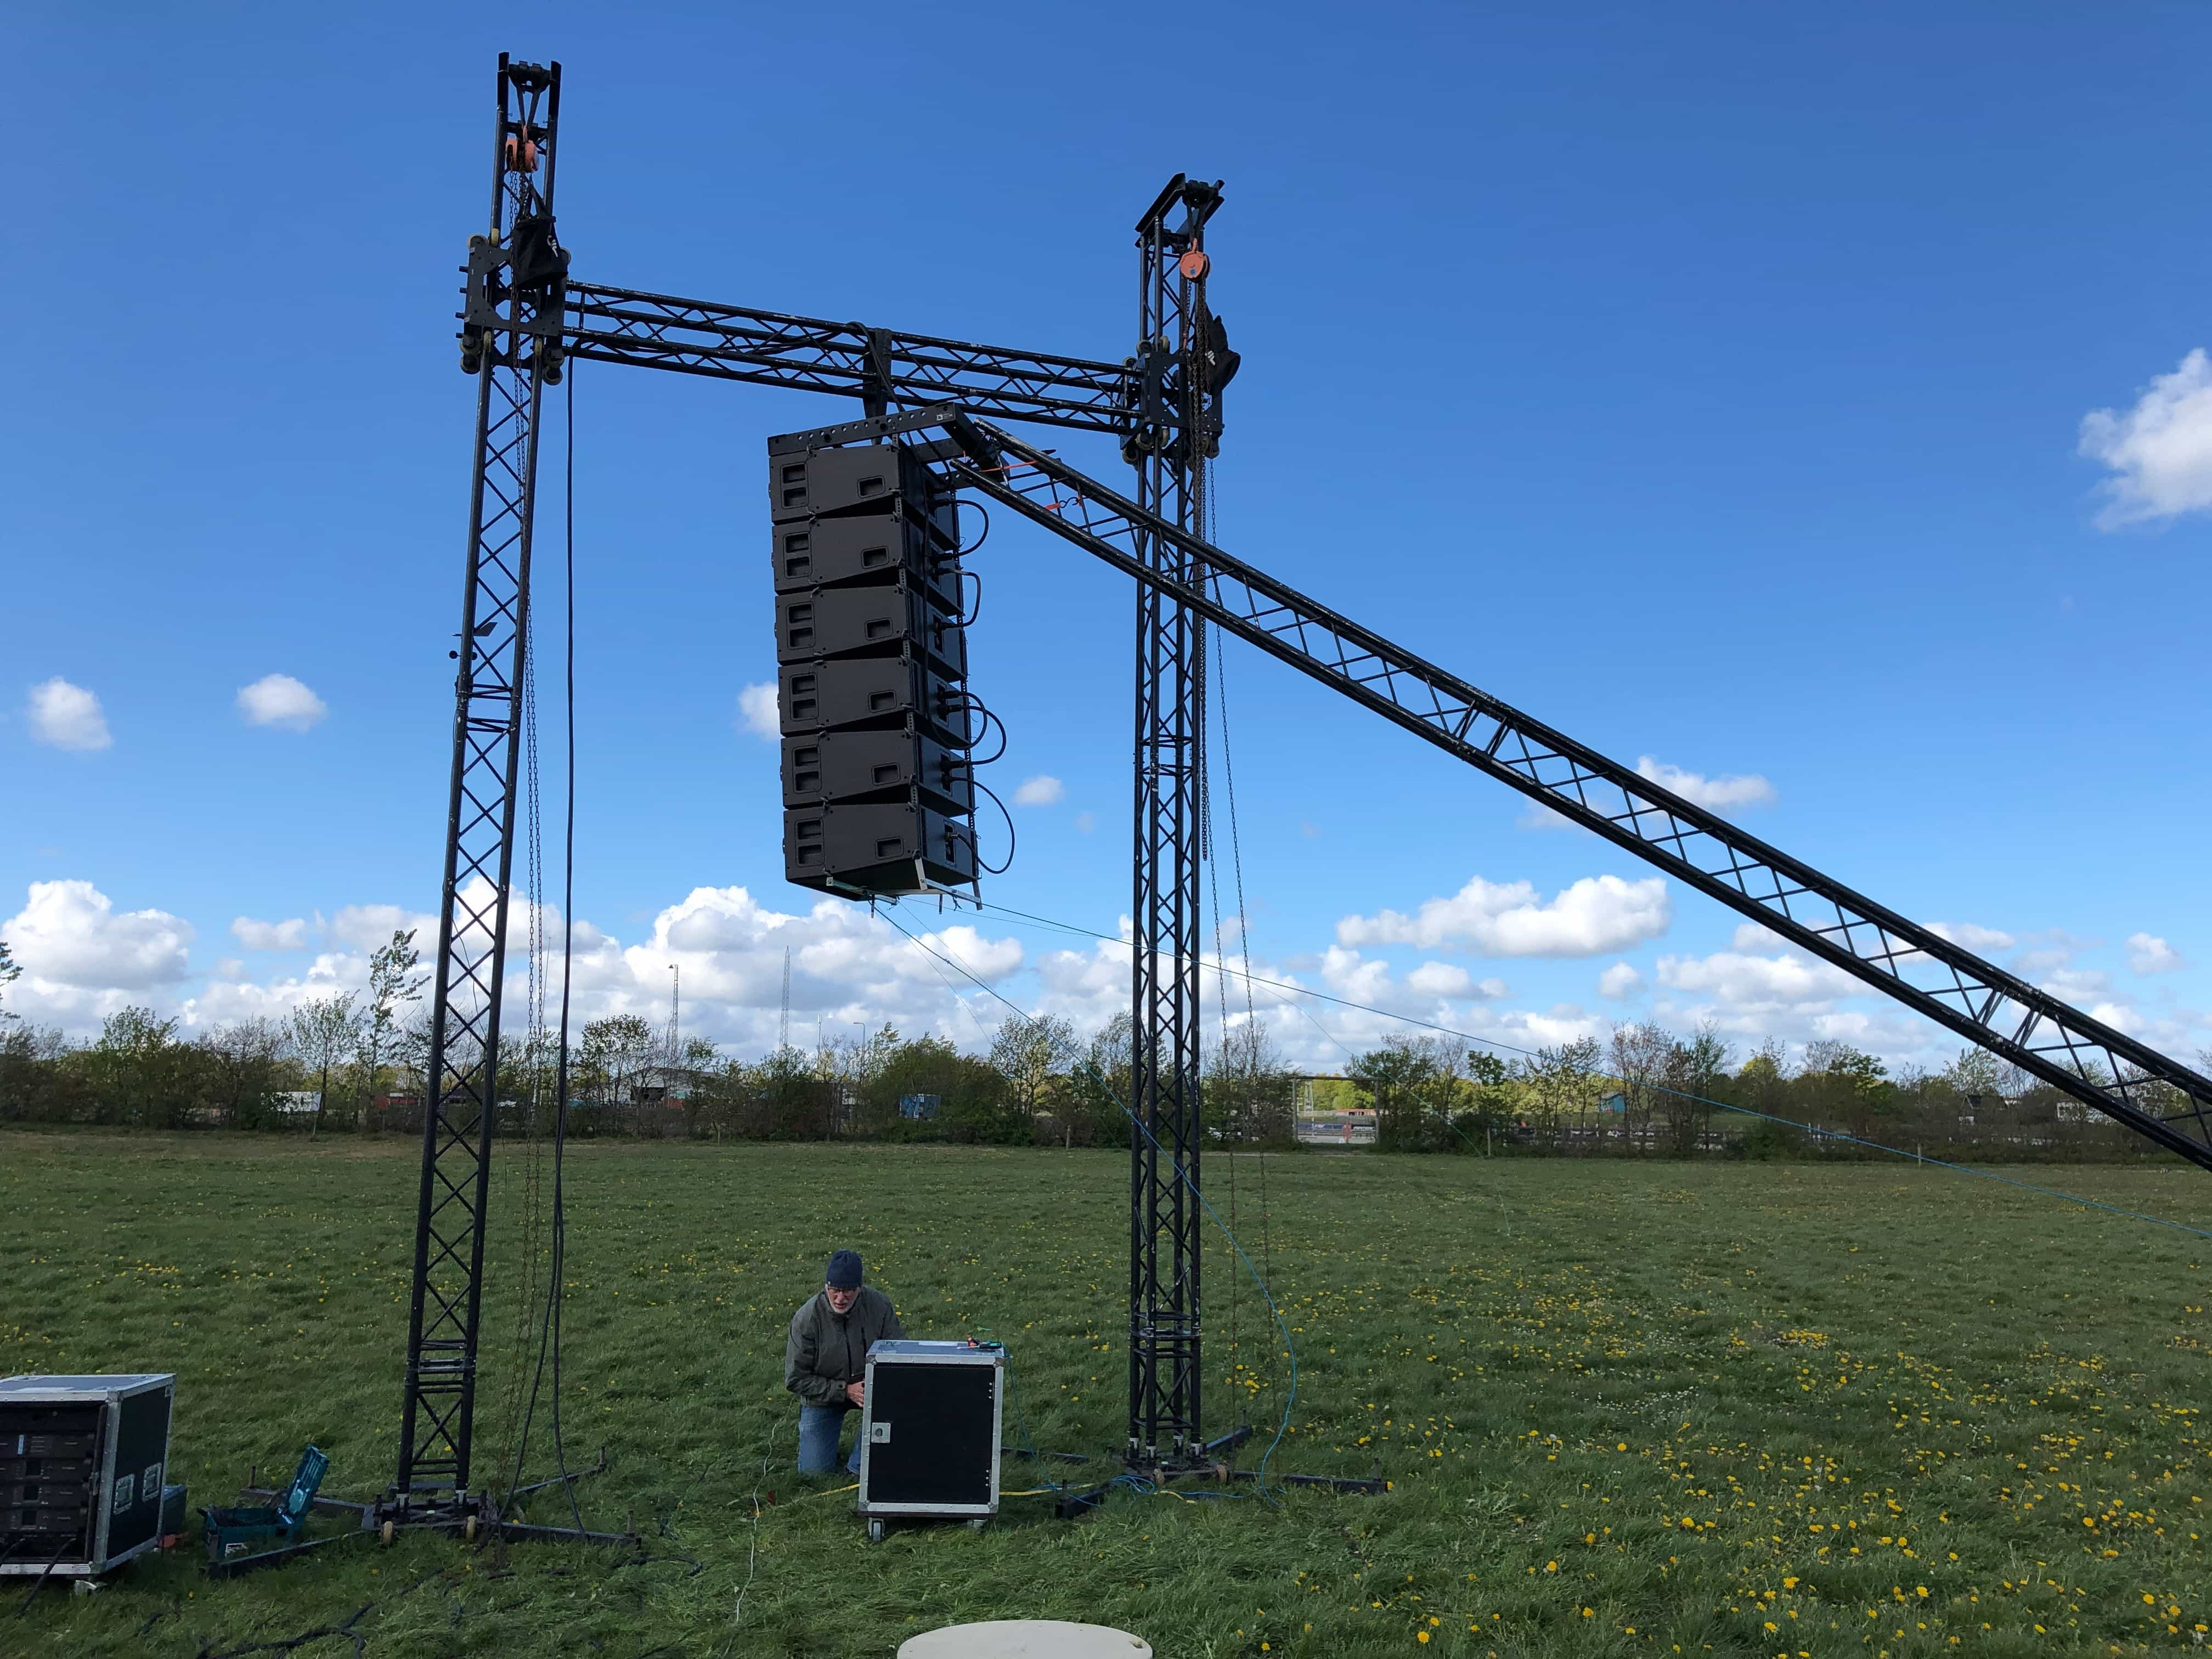
\includegraphics[width=1\textwidth]{IMG_0174}
\end{figure}
    }
  \end{center}
  \vfill
  \begin{center}
  \iflanguage{english}{Aalborg University}{Aalborg Universitet}\\
  \projectFaculty
  \end{center}
\end{titlepage}
\clearpage

\thispagestyle{empty}
{\small
\strut\vfill % push the content to the bottom of the page
\noindent Copyright \copyright{} \projectGroup{}, \projectFaculty{} \projectSemester{}, \AAU{} \the\year\par
\vspace{0.2cm}
\noindent This report is compiled in \LaTeX. Additionally Mathworks \matlab, Inkscape, and Xfig are used to draw figures and charts.
}
\clearpage

{\iflanguage{english}{
\pdfbookmark[0]{Title Page}{label:titlepage_en}
\aautitlepage{%
  \englishprojectinfo{
    \projectTitle %title 
  }{%
    \projectTheme %theme
  }{%
    \projectPeriod %project period
  }{%
    \projectGroup % project group
  }{%
    \projectParticipants %list of group members
  }{%
    \projectSupervisors %list of supervisors
  }{%
    \projectCopies % number of printed copies
  }{%
    \projectCompletion % date of completion
  }%
}{%department and address
  \textbf{\projectFaculty}\\
  Aalborg University\\
  \href{http://www.aau.dk}{http://www.aau.dk}\\
}{% the abstract
  \projectAbstract
}}
{
\pdfbookmark[0]{Titelblad}{label:titlepage_da}

\aautitlepage{%
  \danishprojectinfo{
    \projectTitle  %title 
  }{%
    \projectTheme %theme
  }{%
    \projectPeriod %project period
  }{%
    \projectGroup % project group
  }{%
    \projectParticipants %list of group members
  }{%
    \projectSupervisors %list of supervisors
  }{%
    \projectCopies % number of printed copies
  }{%
    \projectCompletion % date of completion
  }%
}{%department and address
  \textbf{\projectFaculty}\\
  Aalborg Universitet\\
  \href{http://www.aau.dk}{http://www.aau.dk}\\
}{% the abstract
 \projectSynopsis
}}}


\cleardoublepage
\pagestyle{fancy} % Enable headers and footers again
\iflanguage{english}{
\chapter*{Preface\markboth{Preface}{Preface}}\label{ch:preface}%
\addcontentsline{toc}{chapter}{Preface}%
}{%
\chapter*{Forord\markboth{Forord}{Forord}}\label{ch:forord}%
\addcontentsline{toc}{chapter}{Forord}%
}
This report is composed by Jonas Buchholdt during the 10th semester of \projectFaculty{} at \AAU{}. The general purpose of the report is  \textit{\projectTheme}. 

For citations, the report employs the Harvard method. If citations are not present by figures or tables, these have been made by the authors of the report. Units are indicated according to the SI standard.


\vspace{\baselineskip}\hfill \AAU, \today
\vfill\noindent
\begin{center}
\begin{minipage}[b]{0.45\textwidth}
 \centering
  \textit{}\\
 {}
\end{minipage}
\hspace{0.3cm}
\begin{minipage}[b]{0.45\textwidth}
 \centering
  \textit{}\\
 {}
\end{minipage}
\end{center}
\vspace{1\baselineskip}
\begin{center}
\begin{minipage}[b]{0.45\textwidth}
 \centering
  \textit{Jonas Buchholdt}\\
 {\footnotesize <Jbuchh13@student.aau.dk>}
\end{minipage}
\end{center}


%\input{chapters/laesevejledning/_laesevejledning}


\begingroup % Let ToC start on even page.
  \let\cleardoublepage\clearevenpage
	\cleardoublepage
	\iflanguage{english}{\pdfbookmark[0]{Contents}{label:contents}}{\pdfbookmark[0]{Indhold}{label:indhold}}
 \tableofcontents
\endgroup

\cleardoublepage

\printnoidxglossaries

% Mainmatter
\pagenumbering{arabic} % Use arabic page numbering in the mainmatter

\glsresetall

%\printglossaries

 \graphicspath{{figures/analysing/}}
\chapter{Introduction}\label{ch:intro}
Coming later


%%
\part{Problem Analysis and Requirements}\label{pt:analysis} \glsresetall
\graphicspath{{figures/analysis/}}
\chapter{Analysis of sound propogation in outdoor venue}\label{ch:analysis}
%\input{chapters/analysis/...}
\section{Live venue sound challenges}
This section explore the challenges of producing sound in an outdoor environmental. The challenge of producing a good sound experience for the audience highly depend on the calibration method and the atmosphere condition. It is well known that acoustically wave propagation is strongly affected by the inhomogeneous atmosphere doing the outdoor sound propagation. This inhomogeneous atmosphere shifts the calibration of the sound system which affect the intelligibility. In \autoref{sec:ana:aco_liv_ven} an overview of high \gls{spl} \gls{pa} system is discussed.



\subsection{Acoustics as live venue}\label{sec:ana:aco_liv_ven}
An outdoor \gls{pa} system is an important sound reinforcement concept today. It is used to address information, music or just entertainment where the number of audiences is large, sometimes more than 10.000 audiences. The number of the audience makes it difficult to address the information to the large number of audience without reinforcement of the information. The reinforcement is nearly always done from a stage with a large \gls{pa} system and sometimes delay unit in the middle of the audience area. The stage lifts the artist while the \gls{pa} system is designed to cover the audience area with sound. The optimal \gls{pa} system covers the area with a linear frequency spectrum in the audible frequency range with a homogeneous \gls{spl}. Today, the used speaker is a line source array flown in both side of the stage and is therefore only close to the audience in front of the stage. The line source array is an array of small identically wide speakers attached to each other to form a vertical line of speakers. An example of a line source array can be seen in \autoref{fig:ana:flo_kud}

\fig{flown_kudo}{The figure shows an illustration of a KUDO line source array from L-Acoustics \citep{KUDO_manual}}{fig:ana:flo_kud}{0.4}

Every speaker or a small group of the line source array can be controlled individually, both in sound coverage area angle and \gls{spl}. The benefit of the line source array module design is that the coupling between the line source element can be controlled. With an optimized control system of the line source array, the audience area can be covered with sound such that all audience can hear the information. An optimized line source array has, for example, an optimized main lobe such that the lower part of the main lobe lays flat along the audience area.
The following \autoref{fig:ana:aco:liv_ven} shows a graphical illustration of the outdoor \gls{pa} venue concept.

\xfig{analysis/concept_outdoor.pdf_t}{The figure illustrate the concept of outdoor \gls{pa} venue}{fig:ana:aco:liv_ven}{0.65}

As shown in \autoref{fig:ana:aco:liv_ven} the distances from one element in the line source array to the receiving audience dependent on the audience position. This indicates that the signal to every line source element has to be adjusted with respect to the coverage area. This is necessary because the wave amplitude decay with distances and is addressed in \autoref{sec:ana:geo_spr_los}. The adjustment is not as simple as just supply the upper speaker with more power. A sound wave is a mechanical movement of the particle in the air, which condensate and compression the air molecule, then low pressure and high pressure respectively. The movement of the molecule depends on the medium, and in this thesis, the medium is limited to air. The \gls{spl} is the local pressure divination of the instantiates atmospheric pressure. The atmospheric pressure, therefore, set a lower bound on the condensation while very high pressure change the speed of sound and distord the wave as it propagate. To communicate the information without introducing distortion by the lower limit, the maximum amplification is therefore limited by the lower bound of the atmospheric pressure. Luckily the pressure near the ground is typically \SI{101.325}{\kilo\pascal} or a maximum sound pressure of \dBp{194} The movement of the particle in the air depends on the medium in the air. The medium in the air is not constant and varies over time with respect to pressure, wind, humanity and temperature. The analysis starts with the experience for live concert of the author in \autoref{sec:ana:aut_exp_con}, next \autoref{sec:ana:hom_ats_con} address the impact of homogeneous atmospheric effect on sound propagation. Then \autoref{sec:ana:hom_ats_con} address the impact of  inhomogeneous atmospheric effect on sound propagation. 


\subsection{Author experience of live concert}\label{sec:ana:aut_exp_con}
The Author of the thesis has experience with live concert both as an audience and as a sound engineer. The aspect of being the sound engineer and an audience to a live concert is very different. As a sound engineer, the area for controlling the sound is a secured area with a tent as protection. The tent roof often shadows for the high frequency and the walls make standing waves of the low frequency because the distance between parallel tent walls fits with the wavelength for the low frequency. The control area is defined as the \gls{foh}. The \gls{foh} is often equipped with an additional speaker and the sound engineer does not fully know how it sounds outside the \gls{foh} but base there mix on experience. The aspect of being an audience depends on where the audience is with respect to the stage. In close hand to the stage the \gls{spl} is high and often to high especially in the low frequency. The low frequency is often made as a vertical array at the ground or two end-fire arrays and shall be able to exhibit all audience by an audible low frequency spectrum typically from \Hz{25} but one company extends down to \Hzp{13} Therefore the \gls{spl} just in front of the subwoofer has a very high \gls{spl}. This position is not comfortable to be at in longer period and the high \gls{spl} mask the higher frequency. The optimal audience position is in the centre of the stage and not as long from the stage as the delay towers. The average \gls{spl} is often less than \dB{102} since the sound engineer try to keep a maximum average \gls{spl} at \dB{102} just in front of the \gls{foh}. Moreover, it is the stereo sweet spot. This position is the only position where the stereo image is optimal. The stereo perspective problem is a hot topic nowadays, both L-Acoustics \citep{l_acoustics_l_isa} and D\&B Audiotechnik \citep{dbsoundscape} have made there own solution to the problem. The idea is to fly many small line source array above the stage and assign every musician to there own line source array. The concept minimises the interference between two line source array playing the same mono signal. 
Between the delay line towers, the low frequency spectrum is still good and audible but something happens to the high frequency. Often the high frequency disappears for few second and gets back. This phenomenon altering through the full concert. Behind the delay towers, the line source array in the delay tower reproduces the sound such that the audience in the back also gets the high frequency spectrum. The question is why does the high frequency disappear for a short period when the low frequency does not? This thesis will focus on answer this question.

 

\section{Ideal geometric spreading loss}\label{sec:ana:geo_spr_los}
When a line source generates a sound wave, the wave field exhibits two fundamental difference spatially directive regions, near-field and far-field. In near-field, the wave propagates as a cylindrical wave wherein the far-field the wave propagates as a spherical wave. When the wave propagates as a cylindrical wave, the wave propagates only in the horizontal plane, and therefore the attenuation is \dB{3} per doubling of distance. For a spherical wave propagation, the wave propagates in all direction. Therefore the attenuation is \dB{6} per doubling of distance. The near-field and far-field attenuation are based on non-absorption homogeneous atmospheric conditions. The border between the near-field and far-field depends on the hight of the array and the frequency. The distance can be calculated with Fresnel formula \autoref{eq:ana:near_field}, where the wavelength $\lambda$ is approximated to $\frac{1}{3f}$ \citep{bauman2001wavefront}

\begin{equation}\label{eq:ana:near_field}
d_{B} = \frac{3}{2}f \cdot H^{2}\sqrt{1-\frac{1}{(3f \cdot H)}}
\end{equation}

\startexplain
\explain{d_{B}}{is is the distance from the array to the end of near field}{\meter}
\explain{f}{is the frequency}{\kilo\hertz}
\explain{H}{is the hight of the array}{\meter}
\stopexplain

In equation \autoref{eq:ana:near_field} it can be calculated that less than \Hz{80} radiate directly intro spherical wave on the exit of the speaker no matter the hight of the line source array. The following \autoref{fig:ana:near_far_field} shows a horizontal cut of the near-field, far-field from a line source array. 

\fig{near_far_field}{The figure shows horizontal cut of a \gls{spl} radiation pattern of a line source array \citep{bauman2001wavefront}.}{fig:ana:near_far_field}{0.8}

As seen in \autoref{fig:ana:near_far_field}, the wave propagating as a plane cylindrical wave in the near-field, where the coverage area for every double of distance is twice as big. Since the coverage area is twice as big, the \gls{spl} is the half for the doubled distance. When the wave excites distance $d_B$, the wave propagates intro far-field where the coverage area is four times higher while travelling the double of distance and therefore the \gls{spl} is four times less. In far-field, the wave propagates as a spherical sound source  

\section{Homogeneous atmospheric conditions}\label{sec:ana:hom_ats_con}
This section aims to analyse the sound wave propagation in homogeneous atmospheric conditions. It is well known that the sound wave propagation is highly depending on the atmospheric conditions. The propagation depends on the atmospheric pressure, wind, temperature and humanity, where the two latter moreover is frequency dependent. The attenuation difference in frequency for temperature and humanity can be above \dB{80} \citep{corteel2017large}. The following sections introduce a brief discussion of homogeneous atmospheric conditions effect on sound propagation.


\subsection{Humidity and temperature impact}\label{sec:ana:hu_temp}
The temperature and humidity have three impacts on wave propagation from a line source array, directionality of the speaker, the speed of sound and a lowpass effect. The following description starts with the latter. 

\paragraph{Lowpass effect} The effect of humidity and temperature on wave propagation act as a lowpass filter while the wave propagates. The low frequency remains without any additional attenuation where the high frequency highly depends on the atmospheric condition. In other words, attenuation in the high frequency range does not only depends on the spreading loss but also temperature and humanity. Therefore, for long distance, the atmospheric conditions have a high influence on the frequency spectrum delivered to the audience. Humanity and temperature attenuation are already well studied and standardised. Standard \citep{iso_9613-1} gives an overview of calculating the \gls{spl}  attenuation concerning the frequency, distance, temperature and humanity. The article \citep{corteel2017large} gives some examples of attenuation at a distance of \SI{100}{\meter}. The article shows that if humanity increases proportionally to the temperature, the lowpass effect is small. If the change in temperature and humanity is the opposite of each other, for example, high temperature but dry, the attenuation in high frequency is significant. The following \autoref{fig:ana:temp_eg} shows the worst-case scenario from \citep{corteel2017large}.

\fig{temp_worst_case}{The graph shows the attenuation in \db with respect to frequency, humanity and temperature \citep{corteel2017large}.}{fig:ana:temp_eg}{0.9}


As shown in \autoref{fig:ana:temp_eg} the attenuation in the high frequency is significant and excite \dB{30} within the audible frequency range. The attenuation is such markedly that applying more power does not cover the attenuation without an extreme high-pressure driver. That driver might be possible to design in theory but not in practice. Extreme high-pressure drivers introduce high distortion as is explained in \autoref{sub:sec:pre_imp}
 
\paragraph{Speed of sound} The second consequence is the speed of sound. At temperature range from \SI{0}{\celsius} to \SI{40}{\celsius} the speed of sound with respect to humanity change is sparse and mostly only depend on temperature change. At \SI{0}{\percent} humidity, the speed of sound increases with \SI{0.6}{\meter\per\second} for every increasing degree \si{\celsius}. At humanity higher that \SI{0}{\percent} the speed of sound increase with respect to humanity, depends on temperature. At \SI{0}{\celsius} the speed of sound increases with approximately \SI{0.8}{\meter\per\second} when the humidity raises from \SI{0}{\percent} to \SI{100}{\percent}. At \SI{30}{\celsius} the speed of sound increases with approximately \SI{2.7}{\meter\per\second} when the humidity raises from \SI{0}{\percent} to \SI{100}{\percent} \citep{humanity_effect_on_speed} \citep{bohn1987environmental}.  The wave propagation speed start at \SI{331.5}{\meter\per\second} at \SI{0}{\celsius} and \SI{0}{\percent} humanity. The following \autoref{fig:ana:hu_speed} shows the speed of sound with respect to humanity and temperature. 

\plot{code/speed_hum_temp}{The figure shows the increase of sound speed with respect to humanity and temperature \citep{bohn1987environmental}}{fig:ana:hu_speed}

As seen in \autoref{fig:ana:hu_speed}, the effect of humidity is negligible compared to the effect of temperature changes, but as the temperature increases the humidity gets significant. At a temperature of \SI{40}{\celsius} the speed of sound is changed \SI{4}{\meter\per\second} from \SI{0}{\percent} humidity to \SI{100}{\percent}


\paragraph{Directivity} The directivity of a line source array in the mid and high frequency is always controlled mechanically by a horn because the wavelength is short compared to the size of the speaker. At low frequency, the wavelength is too long to be controlled mechanically by a horn. Therefore the directional pattern is controlled via cancellation from a backwards pointing speaker. The directivity of both the subwoofer and the high frequency driver sufferers from temperature increased. At the high frequency, the main lobe gets narrower when the mechanical horn gets warmer, and the effect is notable when the sun directly heats up the horn. The resend that the temperature of the building horn affect the directivity of the high frequency is that the warm horn surface heats the air at the mouth of the horn.  Since the temperature increases, the wavelength gets shorter. Therefore the main lobe of the high frequency gets narrower \citep{levine2018influence}. The directivity of the low frequency is affected as in the high frequency with the temperature increase. The difference is not as significant as in the high frequency since there is no surface heat. The directivity is then not affected due to the sunlight, but only the temperature is increasing and decreasing. As in the high frequency temperature differences change the wavelength, and then the length between the speaker in a cardioid subwoofer does not match the optimised distance between the speaker any more. 



\subsection{Wind impact}
The wind impact is depending on the angle of the wind direction with respect to the direction of sound propagation. A homogeneous wind is a laminar wind flown with the same homogeneous speed. The following analysis assumes homogeneous laminar wind flow from one direction. The analysis is of both oblique wind and parallel wind with respect to the frontal direction of the speaker line source array. The analysis starts with the latter. 

\paragraph{Parallel to sound propagation} When the wind flows in the same direction as the sound wave propagation, the wind flow in \si{\meter\per\second} is an addition to the speed of sound. When the wind flows in the opposite direction, it is a negative addition.  In other cases, the influence is complicated since the wind deflect the sound waves.


\paragraph{oblique- and crosswind} The effect of oblique- and crosswind on sound wave propagation is rarely studied, and the effect on high frequency seems to be unclear. Few author have addressed the problem in a simulation of traffic noise and by practical experience \citep{effect_of_wind}, \citep{crosswind_effect_2016}, \citep{BALLOU2008xi}. They found that the crosswind effect might refract the wave in the wind direction over distances. Furthermore, they found that the effect is not linear in frequency. The author of \citep{BALLOU2008xi} indicates that the frequency dependency might be due to the directionality of the high frequency drivers. The author of \citep{crosswind_simulation} has simulated the homogeneous crosswind effect on a omnidirectional source at \Hz{100}. The author of \citep{ray_tracing} implemented a ray tracing method with a vector based interpolation as shown in \autoref{fig:ana:cal_wav_dir}.



\xfig{analysis/cal_of_crosseffect.pdf_t}{The figure shows a geometrical calculation scheme of calculate the resulting wave direction at crosswind \citep{ray_tracing}, \citep{crosswind_simulation}}{fig:ana:cal_wav_dir}{0.5}
\startexplain
\explain{c}{is the speed of sound}{\meter\per\second}
\explain{n}{is the normal unit vector}{\meter}
\explain{v}{is the speed of wind}{\meter\second}
\explain{v_{ray}}{is the resulting sound ray}{\meter}
\stopexplain

As it is seen in \autoref{fig:ana:cal_wav_dir} the ray vector $v_{ray}$ is an addition of the sound speed vector $c \cdot n$ and the speed of wind $v$. The wave speed and wave length therefore depend on the speed of wind and the angle between the wind and the sound propagation. The following \autoref{eq:ana:wind_angle} calculate the speed of sound with respect to the angle and wind 


\begin{equation}\label{eq:ana:wind_angle}
c_r = c+||v||_2 \cdot sin(\theta) = ||c \cdot n + v||_2 = ||v_{ray}||_2
\end{equation}

\startexplain
\explain{\theta}{is the angle of the wave with respect to the wind}{\degree}
\explain{c_r}{is the resulting speed of sound}{\meter\per\second}
\stopexplain



As the wave propagating, the resulting $v_{ray}$ increases in the direction of the wind. The article \citep{crosswind_simulation} simulates the effect of crosswind in a \gls{fdtd} simulation with a wind speed of \SI{102.9}{\meter\per\second}. For the acceptable condition to a concert the wind speed is less than \SI{20}{\meter\per\second} otherwise, the concert is stopped for safety. The following simulation \autoref{fig:ana:cro_win_sim} shows the simulation result from \citep{crosswind_simulation}. The source is an omnidirectional \Hz{100} spherical source while the wind has a constant uniform wind speed from left. The simulation is done in two dimensions. 


\fig{crosswind_simu.pdf}{The figure shows a simulation of a \Hz{100} omnidirectional source with a uniform constant wind speed from left with speed of \SI{102.9}{\meter\per\second} \citep{crosswind_simulation}. }{fig:ana:cro_win_sim}{1}

It is seen in \autoref{fig:ana:cro_win_sim} that the crosswind do not affect the direction of the wave from a low frequency spherical source. It only affects the time of arrival to the audience.




%The procedure of calculating the resulting wave vector $w$, is to project the wind vector $d$ intro the direction of the wave vector without wind $a$. The projector \textcolor{red}{$p$} is used to calculate the orthogonal $e$ which make the calculation of the wave vector $w$ easier compare to the wind vector $d$ which is not orthogonal to $a$. $e$ is simply calculated with addition between $d$ and \textcolor{red}{$p$}. The next step is to calculate the wave vector $w$. The  wave vector $w$ shall be calculate by the $a$ and $e$ but the length of $a$ is unknown. Therefore the length have to be founded and a way to find the length is the knowledge of $w$. $w$ have to be the same length for every new simulation step. For simplicity in the explination the length of $w$ is assumed to be \SI{1}{meter}. By using the sinus relation the $argsin$ to the length of $e$ gives the length of $a$. Since the simulation only is in two dimention, the resulting wave direction is then an addition between $a$ and $e$. To be able to find the limit length of the wave vector $w$, a resolution option is incorporated in the calculation as \texttt{res}

%The used calculation script is as \autoref{code:ana:spe_cov}.
%
%\includeCode{crosswind_geo.m}{matlab}{20}{27}{The speaker coverage area simulation code}{code:ana:spe_cov}{./code/}
%
%To find the limit value of the wave vector $w$ a simulation is made with different length of $w$. The following \autoref{plot:ana:lim_fin} shows the wave vector $w$ for different length and a simulation of \SI{200}{\milli\second}.
%
%\plot{plot/limit_finder}{The graph shows the wave vector $w$ with \SI{90}{\degree} angle and a crosswind from left with a speed of \SI{10}{\meter\per\second} and a wave propagation time of \SI{200}{\milli\second}. A length less that \SI{0.1}{\meter} is not visible in the graph and is therefore not calculated}{plot:ana:lim_fin}
%
%Based on the wave propagation differences in \autoref{plot:ana:lim_fin} it is decided that the used limit is \SI{0.5}{\meter}. A simulation of the speaker coverage area is shown in \autoref{plot:ana:spe_cov_area}
%
%\plot{plot/speaker_cov}{The graph shows the coverage area of two speaker with \SI{90}{\degree} angle and a crosswind from left with a speed of \SI{10}{\meter\per\second} and a wave propagation time of \SI{189.3}{\milli\second}}{plot:ana:spe_cov_area}
%
%
%It can be seen in \autoref{plot:ana:spe_cov_area} that the coverage area distance is reduces to \SI{53}{\meter} when the speaker have an angle of \SI{90}{\degree} and the the wind speed is \SI{10}{\meter\per\second}. Another important aspect which is changed is the wave travelling distance from the speaker to the audience. Without wind the distance along the first ariavle wave is  \SI{53}{\meter}. When the wind is present, the sound ariving to the audiance at \SI{53}{\meter} is the wave vector, which have traveled longer that the wavev arriving to the audiance without wind. The wave traveling is increased by \SI{6}{\meter}. This increase in length introduce attenuation in the \gls{spl} arrival to the audience.

%refraction that's a direct result of Snell's law

\subsection{Pressure impact}\label{sub:sec:pre_imp}
The influence of atmospheric pressure change is low compared to the effect of wind, humanity and temperature. The average attenuation from \Hz{4000} to \Hz{16000} with fixed temperature was \dB{2} while going from \SI{54.02}{\kilo\pascal} to \SI{101.33}{\kilo\pascal}. The atmospheric pressure then only have a negligibility influence on sound propagation and is generally not frequency dependent. 

Beside the small impact of pressure difference in the atmosphere, the high pressure generated by the speaker does have a tremendous influence on the sound propagation. There are two main places in the propagation way that can produce distortion concerning the pressure. The design of the high frequency horn \citep{czerwinski1999air}, the port design of the low frequency driver \citep{vanderkooy1998nonlinearities} and the influence of the sound path. The following description starts with the latte.

\paragraph{Sound path} In the sound path, two main factors cause distortion in the wave propagating. As described in ... a sound wave is condensation and compresses the air particle. The air medium has a lower limit that cannot be less than a vacuum. Therefore the higher bound of \gls{spl} is depending on the atmospheric pressure. As an example, at \SI{54.02}{\kilo\pascal} the highest \gls{spl} before distortion caused be vacuum is \dB{188.6} and at \SI{101.33}{\kilo\pascal} the highest \gls{spl} before distortion caused be vacuum is \dB{194.1}. 

There is therefore a higher limit determide by the atmospheric pressure to vacuum, but this is not the only limit for distortion. Very high pressure in the comparation also distorte the sound. At the comparation seriusly signal deterioration orccore if the amplitude is high. The distortion of the comparation is explained by the lack of linear dependency between the particle velocity and the \gls{spl} in a sound wave. The \gls{spl} increases more that the dencity of the sound wave which causeing the condensation of the sound wave to be stiffer and therefore propagate faster than in the condencation of the wave. This effect cause that the speed of sound to travle faster in the comparation and slower in the condencation and produce hamonic distiortion. The haminic distortion is by this effect is even present in \gls{spl} less than \dB{120} \citep{czerwinski1999air}.
The effect is athat the sine wave transformes to a sawtoorh as it propagate which transfer energy to the hamonic of the propagation wave. The distortion is not only \gls{spl} dependent, but also depend on the frequency. The higher the frequency is the the faster the sinosoid transformes intro a sawtooth and tharefore the distortion increases with frequency for similar \gls{spl}. The harmonic distortion of the fundemental sinosoid is frequencies that is the the double, second order and the third order harmonic. Thoes frequenci is higher than the fundemental frequency and therfore as explained in \autoref{sec:ana:hu_temp} have  ahigher attunation with respect to the distance. In most cases the attunation is not as high as the increase of the hamonic distortion and therefore the distortion of the wave propagation is not conpensated by the viscus losses but does that the distortion is not as drastical as it would have been without viscus losses \citep{czerwinski1999air}. The distortion made by air propagation is much less than the distortion in the mouth of the speaker which leeds to the next distortion problem produced by high pressure \citep{czerwinski1999air}.

\paragraph{Driver throught and mouth design} High pressure in both horn phase plug, seald enclosures and vented enclosures or reflex enclosures for low frequency driver cabinet produce distortion as they act as nonlinear components. The latter produce distortion because high pressure makes air turbulence in the vent. By the optimal design the distortin of turbulent flow can be kept low \citep{roozen1998reduction}. The turbulence phenomena does not only cause in the mouth of the low frequency driver, it also occore in the phase plug of the compression driver if the \gls{spl} is high \citep{czerwinski1999air}. The distortion depend on the air's moving mass, the stiffness and the viscus losses on the diagram displasement and the \gls{spl}. As the air in the hifh frequency driver comprrssion it become heavier, stiffer and thicker which make nonlinear wave propagation. It typical occore when the compression chamber exceeds approximatly \dB{170}. At higher level the particle velocity resistance to teh iar flow increases and the laminar air flow turns intro turbulent air flow. The distortion is also dependning on the length of the horn and the expantion rate of the horn flare. To keep the distortion as low as possible for the high frequency driver the displacement of the diaphragm should be kept significant lower than the hight of the compression chamber \citep{voishvillo2004comparative}. Therefore, to keep the displacement of the high frequency driver as low as possible, the frequency range should be limmited as high as possible since the displacement gets lower as the frequency increases.



\subsection{Ground absorption and reflection} 
In a concert area, ground absorption and reflection is complex because there is two very different situations. Before the concert the area is a locally plan area often with mown grass and with ground reflection.  An examples of frequency response in the hight of an audience or measurement microphone is given in \citep{review_of_sound} where it is seen that the ground reflection does have a high effect while playing over mown grass. A measurement in \autoref{ch:ap:measurement_one} and \autoref{ch:ap:measurement_two} is also preformed where the ground reflection clearly have a big influence on the recieved frequency response. Doing the concert the intersting part is not such ground reflection effect but the audience reflection or absorbtio.  The area along the concert is packed by audience, and is therefore not easy to calculate. The absorbtion and reflection in an outside concert area with audience is rearly studied but absotbtion for the audience inside a concert hall have been highly studied \citep{audience_abso}. The absorbtion of the audience is founded to be high in all measured concert hall from \Hz{1000} octave band and abwards to the highest measured octave band in \citep{audience_abso}. The avearge absorbtion $a_{sabine}$ coefficient is calculated to be above 0.80. The method and result can be founded in \citep{audience_abso}. The reflection in the high frequency in the audeince area doing concert is therefore assumed to be very low. At low frequency the article \citep{audience_abso} indicate that the absorption decay with frequency beneath  \Hz{250}, but The octave band for low frequency driver is \SI{31.5}{\hertz} but is not measured by \citep{audience_abso}. The low frequency absrobtion at \SI{31.5}{\hertz} octave band is therefore assumed to low even in the normal position of the low frequency driver. They are often situated in front of the stage on a line or in end fire settings, often with a maximum distance of half the wavelength from acoustical center to acoustical center. The distance between the low frequency driver is determinde by the half wavelength of the highest frequency, such that they radiate a plan wave \citep{bauman2001wavefront}. Higher distance between acoustical center will cause interference in the low frequency in the audience area. 



 
 \subsection{Homogeneous speed equation}\label{sec:ana:inhom_ats_con}
 The following \autoref{eq:ana:wind} calculate the speed of sound based on homogeneous temperature and wind speed.

\begin{equation}\label{eq:ana:wind}
c =  c_0 \sqrt{1+t/t_0} + u \cdot sin(\theta)
\end{equation}  

\startexplain
\explain{c}{is the resulting speed of sound}{\meter\per\second}
\explain{u}{is the speed of wind}{\meter\per\second}
\explain{c_0}{is the speed of sound at \SI{0}{\celsius}}{\meter\per\second}
\explain{t}{is the temperature}{\celsius}
\explain{t_0}{is the temperature at \SI{0}{\celsius} (273.15)}{\kelvin}
\explain{\theta}{is the angle of wind with respect to the wave propagation}{\degree}
\stopexplain


 
\section{Inhomogeneous atmospheric conditions} 
The aim of this section is to analyse the sound wave propagation in inhomogeneous atmospheric conditions. In an inhomogeneous atmosphere, the pressure and speed is a function of position. By this fact, the modelling of a sound wave is very complex and depend on various variables such as temperature and wind speed. The following sections give a short introduction to the effect of inhomogeneous atmospheric conditions. 
 
 
\subsection{Atmospheric refraction} \label{sec:ana:atm_ref}
When the wind speed, the temperature and humanity is assumed to be homogeneous in the sound field, the sound is travelling in a straight path. Often this is not true, the wind speed increases logarithmically with the hight from the ground to the geostrophic wind \citep{asmos_acous_2016} in the free troposphere \citep{spr_hand_book} and the temperature and humanity are inhomogeneous. The geostrophic wind in the free troposphere is located in a hight from approximately \SI{1}{\kilo\meter} above the ground \citep{spr_hand_book}, \citep{geostrophic_wind}. The inhomogeneous atmospheric condition makes the speed of sound to depend on the hight from the ground. This results in a curved sound path and is called as atmospheric refraction. For small distances, the atmospheric refraction has a spars effect on the sound travelling path, because the speed of sound is much faster than the speed of the wind and the temperature change. Generally distance up to \SI{50}{\meter} is often assumed to have no significant refraction effect \citep{effect_of_wind}. For distances larger than \SI{50}{\meter} the refraction is assumed to have a significant influence, especially when the sound source and the receiver are close to the ground. Refraction is frequency and distance dependent and is measured in \db excess attenuation. The means of excess attenuation is that only the effect of wind or temperature is considered, all other atmospherical effect is excluded. A measurement is given in \citep{review_of_sound} for a point source where the wind speed is \SI{5}{\meter\per\second}. At a distance of \SI{110}{\meter}, it is observed that frequency above \Hz{400} is refracting where frequency below is rearly effected of refraction. Moreover, at a distance of \SI{615}{\meter} the refraction is present in the full measured frequency range from \Hz{50} to \Hz{3200}. In the perspective of live concert the intersting distance is the \SI{110}{\meter} from the line source array to the audience rather than the \SI{615}{\meter}. Both the downwards and upwards refraction is intersting. In the upwards refraction the audience might be in the shadow zone where for the downwards refraction the high frequency reflection from the ground is asumed to be low when the concert area is full of audience. Therefore the high frequency is refracted down intro the frontal audience and no reflection of the high frequency propagate to the back part of the audience. The following \autoref{fig:ana:shadow_zone} display the phenomena of upwards refraction.


\xfig{analysis/shadow_zone.pdf_t}{The figure illustrate the shadow zone occure from a upwards refraction. A line source speaker array contains of many couplet point sources. Every lowest sound path dashed line indicate the lower directional angle of one poins source in the line source array.}{fig:ana:shadow_zone}{0.73}


The following description is based on the distance of \SI{110}{\meter} and upwards refraction. As explained in \citep{review_of_sound} the refraction at a distance of \SI{110}{\meter} is highly frequency dependent. At frequency below \Hz{400} the effect is sparse but above the effect is high and may result in \dB{20} attenuation at the audience. The reason that the refraction is frequency dependent is that the scale of the wind gradient and temperature gradient close to the ground is small compare to the wavelength of the low frequency \citep{review_of_sound}. This theory does not follows the shell's law. Shell's law describe the refraction as a layer change in the medium of propagation. Shell's law of refraction is defined as \autoref{eq:ana:shell_law}

\begin{equation}\label{eq:ana:shell_law}
\frac{cos(a_1)}{c_1} = \frac{cos(a_2)}{c_2}
\end{equation}

\startexplain
\explain{a_1}{is the input angle in the horizontal plan}{\degree}
\explain{c_1}{is the sound of speed in the medium of arrival}{\meter\per\second}
\explain{a_2}{is the output angle in the horizontal plan}{\degree}
\explain{c_2}{is the sound of speed in the medium of destination}{\meter\per\second}
\stopexplain

As it can be seen in shell's law \autoref{eq:ana:shell_law} the frequency dependency is not a factor and ether shell's law is only a approximation or the frequency dependency does not apper fron only laminar wind flow profile. The article \citep{review_of_sound} only explorer frequency upto \Hz{3200} but since the refraction depend on the wavelength, the distance of refraction wave might be much smaller for high frequency. The attenuation with respect to refraction seems to have a saddle attenuation at \dB{20}. A measurement in \citep{review_of_sound} shows the attenuation for the center frequency of \Hz{1200} with \octave{3} band filtered airplain noise. The measurement is interesting with respect to a concert area and is therefore shown in \autoref{fig:ana:excess} 


\fig{excess}{Excess attenuation measured for aircraft noise in the \Hz{1200} \octave{3} band for the ground-to-ground configuration. The vector component of the wind velocity in the direction of propagation for $\blacktriangle$ is \SI{5}{\meter\per\second}, $\square $ a is \SI{0}{\meter\per\second}, and $\triangledown$ is \SI{-5}{\meter\per\second}. The temperature profile is neutral. $F_s$ is the shielding factor, B is the shadow boundary \citep{review_of_sound}}{fig:ana:excess}{0.7}

The following two paragraph explains the difference between wind refraction and temperature refraction.

\paragraph{Temperature} Temperature decresses with respect to the hight at day time and increases at the night time. The increase or decrease can usually be approximated as a logarithmic function. In the day time, the sun heats the ground even at a cloudy day, and the concert area is full of audience. Therefore, the eath and audience radiate warm air, which makes the temperature at a low hight warmer than the temperature at higher hight. This phenomena is named lapse where the uppersite is defined as inversion. As explained in \autoref{sec:ana:hu_temp}, the speed of sound depends on the temperature. Therefore, at day time, the speed of sound in this situation decay with respect to hight. The speed change can be moddled as a change of layer for a plan wave. The output angle of the layer change follows the shell's law. Therefore when the temperature profile is logatrimic the layer change is a function of hight and change the wave direction. The wave direction of the descript weather condition result in an upwards refraction. Since the temperature is a scalar quantity uniformly over large area and a function of hight, an identical temperature profile is aplicable all around the sound source. Therefore the upwards refraction is uniform all along the speaker in the horizontal plane. The following \autoref{fig:ana:temp_ref} illustrate the phenomena where the temperature decay with respect to the hight.
\xfig{analysis/refraction_temp.pdf_t}{Wave refraction in inhomogeneous temperature with lapse profile}{fig:ana:temp_ref}{0.9}
When the temperature profile is reversed, the refraction will be downwards. 


\paragraph{Wind} With respect to the wind speed, a concert area is often a protected area with for example barrier, stage and building. This blockage and the ground friction slows down the wind speed near the ground. Moreover, from nature itself, the wind speed is often logarithmically increased with respect to the hight. When the wave is propagation in the same direction as the wind, the atmospheric refraction refracts the sound wave downwards. When the wave propagates against the wind, the atmospheric refraction refracts the sound wave upwards. The following \autoref{fig:ana:wind_ref} shows the phenomena when the wave propagates against the wind.

\xfig{analysis/refraction.pdf_t}{Wave refraction in inhomogeneous logarithmically increasing wind profile where the wind gradient points towards left}{fig:ana:wind_ref}{0.9}

As shown in \autoref{fig:ana:shadow_zone} the refraction is upwards when the wind flows in the opposite direction as the wave propagation. Behind the line array source, the refraction is downwards and is therefore different than for temperature refraction. The rafraction of wind is the most dominant at a distance of \SI{110}{\meter}. The following \autoref{fig:ana:fre_dep_exc} shows an excess attenuation plot of both inhomogeneous wind and lapse temperature profile. 

\fig{frequency_dep_excess}{Observed attenuation of aircraft noise in a ground-to-ground configuration under a variety of weather conditions. Calculated losses from atmospheric absorption and spherical spreading have been subtracted from the attenuation measured in \octave{3} bands for distances of \SI{110}{\meter} and \SI{615}{\meter}. The numbers on the curves indicate the vector component of the wind velocity in the direction of propagation in \si{\meter\per\second}. All curves are for neutral conditions of temperature except for those marked L, which are for lapse. \citep{review_of_sound}}{fig:ana:fre_dep_exc}{0.7}

It can be seen in \autoref{fig:ana:fre_dep_exc} that the refraction effect at a distance of \SI{110}{\meter} starts at \Hz{400}. The reason that sound enters the shadow zone is not fully understood, but one theory is that the shadow boundary wave is diffuse and therefore significant amount of sound energy enters the shadow zone in turbulent weather. In a non turbulent atmosphere condition the \gls{spl} inside the shadow zone is attenuated well more than \dB{30}. Close to the ground the atmosphere condition is always turbulent because of ground friction. The turbulence wind diffuses the sound wave and change the direction of propagation. The wave that enter the shadow zone can be consitered as creeping wave in turbulent senario. The creeping wave will by them self also refract and therefore be parallel to the the other refraction waves. \citep{tur_on_sound}




\paragraph{Oblique- and crosswind} The effect of oblique- and crosswind on acoustical wave propagation in inhomogeneous atmospheric conditions are rarly studied. The author in \citep{review_of_sound} explain that the refraction is directly zero when crosswind is present, and increase progrative as the direction of propagation deviate from the angle of crosswind. 

Since the effect of crosswind on a line source array speaker is rarely studied, a measurement in windy condition is preformed. The measurement is done over mown grass in a large open area used for football. The used measurement technique is done according to \citep{gunness2001loudspeaker} where more than one impulse response is measured and the mean is calculated by allign the impulse response in time. The wind was considered as strong for outdoor concert. The wind speed was measured to  \SI{14}{\meter\per\second} doing the full measurement. The measurement was done with a four element line source array one meter above the ground. There was used two microphone, where both was situated \SI{23}{\meter} from the speaker, beyond the limiting high frequency directional angle of the speaker. The speaker was placed to propagate in direct crosswind and the microphone was placed on both side of the speaker as shown in \autoref{fig:ana:position}

\xfig{analysis/measurement_one.pdf_t}{The figure shows the microphone position versus the position of the line source}{fig:ana:position}{1}   


The measurement was done according to the description in \autoref{ch:ap:measurement_one}. The measurement was preformed in to step, two measurement within the speaker high frequency directional angle and three outside the speaker high frequency directional angle. The first measurement is shown in \autoref{fig:ana:mea_two_one}. The other four measurement result can be seen in \autoref{ch:ap:measurement_one} and \autoref{ch:ap:measurement_two}. They show same tendency but the difference between the measurement is more drastical in the measurement outside the high frequency directional angle. 

%\plot{plot/measurement_one_one_ana}{The graph shows the average of the first transfer function measurement routine https://asa-scitation-org.zorac.aub.aau.dk/doi/pdf/10.1121/1.381455?class=pdf}{fig:ana:mea_one_one}

\plot{plot/measurement_two_one_ana}{The graph shows the first transfer function measurement within the high frequency directional angle. The $L_{eq,5}$ \gls{spl} different between the microphones is \dB{4.41} (IR_3)}{fig:ana:mea_two_one}

It can be seen in \autoref{fig:ana:mea_two_one} that the general \gls{spl} is higher for microphone 1. Furthermore microphone 1 also shows the typical downwards refraction ground reflection interference in the frequency response which is very similar to the calculated ground reflection interference in \citep{review_of_sound}.  Microphone 2 does not have the same strong interference in the low frequency and the general \gls{spl} is lower than microphone 1. This indicate upwards refraction and some ground reflection. There was done five measurement, The resulting $L_{eq,5}$ \gls{spl} difference is shown in \autoref{ta:ana:spl_dif}.

\begin{table}[H]
\centering
\caption{The table shows the measured $L_{eq,5}$ \gls{spl} for all measurement and the difference between the microphone}
\begin{tabular}{l|l|l|l}
Measurement number &  Mic 1 $L_{eq,5}$ & Mic 2 $L_{eq,5}$ & Difference\\ \hline
        \measurement{fig:ap:mea_one_one}{1}    	&  \dB{71.82} 	&  \dB{66.33} & \dB{5.49} \\
         \measurement{fig:ap:mea_one_two}{2}  	&  \dB{69.09}  	&  \dB{64.69} & \dB{4.40} \\
        \measurement{fig:ap:mea_one_thr}{3} 		&  \dB{67.67} 	&  \dB{63.44} & \dB{4.23} \\
         \measurement{fig:ap:mea_two_one}{4}   	&  \dB{68.10}  	&  \dB{63.69} & \dB{4.41} \\
         \measurement{fig:ap:mea_two_two}{5}   	&  \dB{68.44}  	&  \dB{63.62} & \dB{4.81} \\ 
 Average &   \dB{69.02} &   \dB{64.35} &   \dB{4.67} 
\end{tabular}
\label{ta:ana:spl_dif}
\end{table}

As it is shown in \autoref{ta:ana:spl_dif}, the $L_{eq,5}$ \gls{spl} is higher for microphone 1 in all measurement. Moreover the average $L_{eq,5}$ \gls{spl} difference is \dB{4.67} while for A-weighted $L_{Aeq,5}$ \gls{spl} the average difference is \dB{6.17}.

With respect to the intelligibility frequency range, a weighting filter is designed to obserbe the \gls{spl} differences in the critical intelligibility frequency range. The filter is based on the founded intelligibility frequency range in \citep{arl_us_army}. It is shown in \citep{arl_us_army} that the critical intelligibility frequency range lays between \Hz{1000} and \Hz{4000}. The designed intelligibility weighting filter is a 8\textsuperscript{th} order band pass filter with lower crossover frequency at \Hz{1000} and higher crossover frequency at \Hz{4000}. The resulting average difference is \dB{7.88} and the maximum difference is \dB{9.95}.



\paragraph{Turbulent} Turbulence is a atmospheric condition where the wind eddies. It often starts with large eddies and prograsively brakes down as a cascade effect to smaller and smaller eddies which only depend on the local region. When the eddies is as small as \SI{1}{\milli\meter} the energy dissepears in viscosity and thermal conduction. A statistically distribution of the eddies is defined as turbulence. The turbulence wind flow is therefore a chaotic and stochastic process by the nature and is pressent all the time. It can occur because of change in landscape, stage and blockage, but can also be a process of flow speed increase in the wind, which make the wind to refract on itself. Turbulence is often high at a windy afternoon day and low under the inverse of lapse. Turbulence also often occore near the ground because the ground surface slow down the speed of wind by the friction to the ground. The effect of turbulence on sound is known to make phase and amplitude fluctuation of pure tone. The fluctuation increases with distance until the standard divination of the phase fluctuation is comparible to \SI{90}{\degree} \citep{review_of_sound}. At this point the phase correlation for each sound path is uncorrelated



%\citep{lemke2017adjoint}







\section{Calibration of sound system}
This section analyses the calibration method, which is used by a selection of some Danish sound company. By experience of the author, the hypothesis is that the sound system is calibrated in one point and the microphone is placed just in front of the \gls{foh}. The \gls{foh} is often a little tent, where the sound engineer controls the sound system. The tent is only open in the direction of the stage and reflection might occur from the tent ceiling to the calibration microphone. 

\section{Sound pressure level measurement doing the concert}


\chapter{Summary of Problem Analysis}\label{ch:analysis:summary}

The analysis started addressing the general used method for live concert. It is found out that love concert today use line source array system to cover the audience area with sound. It is observed that a line source array is flown above the audience at the main stage and at a large concert delay tower line source array is used and placed in the middle of the audience. It is founded that a line source array is constructed of many identically speaker attached to each other in a vertical line. Based on the speaker set up the distance from every audience to the speaker depends on the position in the concert area. Therefore the distance from the speaker and the audience depends on the audience and therefore the sound system have to be optimized such that the \gls{spl} coverage is equaly in all position. The following analysis in ... founded that a homogenious \gls{spl} among all audience is an imposible senario but the \gls{spl} among all audience might be possible to optimized by knowledge of the condition of the atmosphere and make up for the spredding lose. 


The experence of the author is included as knowledge for the analysis. It is observed by the author that the wind condition at a concert has a large influence of the experience of the concert. At the low frequency the influence is sparse where for high frequency the effect of the atmospherical condition have a big influence especially when the distance from the speaker is increesed. The figh frequency blowes away for periods ad comes back again. 

A short introduction to the stereo sweet spot problem is also discused. It is a hot topic today among some of the large speaker factorys but the solution require heavily amount of speakers and flying tools. 


The analysis of sound from a line source array started by the ideal geometric spreading loss. Here it is founded that the sound propagation of the line source array highly depend on the hight of the source. The line source array propagate differently with respect to frequency. At a surtain hight of the line source array the propagation is a cylendrical propagation until a surtain distance from the sorce where it starts propagating as a espherical source. In the cylendrical propagation the sound filed as defined as near-field while in the spherical propagation the sound field is defined as far field. 

In the non ideal senario the line source array propagate in ether a homogeneous atmospherical condition or in an inhomogeneous atmospherical condition. 


In the homogeneous atmospherical condition it is founded that the temperature, humidity, pressure and wind influence the sound field. The effect of temperature and humidity is close cubled on sound propagation. When the tamperature is high and the and the humidity is low the air have an large high frequency absorbsion whereas when the temperature and humidity both is eather high or low the  absorbsion is much less. The second effect the temperature and humidity have on sound propagation is the speed of sound. The higher the temperature is the higher the sound of speed is. At \SI{0}{\percent} humidity the speed of sound incerasses with approximatli \SI{0.6}{\meter\per\second} for every \si{\celsius} increase. The effect of humidity also effect the speed of sound by increaseing speed of sound by incerasing humidity but the speed incerse is neglible compare to the temperature effect. Thudermore effect of speed difference in sound propagation change the wavelendth and therefore the directivity of the speaker is changed, but the change is minimal. 

The effect of wind seems to have a sparse effect on the sound propagation when and only when the wind is homogeneous. It is founded that the speed of wind effect the speed of sound. if the wind mowes in the direction of the sound propagation the wind speed is and addition to to speed of sound to find the resulting propagation of speed of sound. In the uppesite cace the speed of sound is lowered. In the case of oblique- or crosswind the effect seems to be unclear for high frequencies. One author has simulated a low frequency spherical source and founded that the only effect is the time of ariavle to the audience.   


The impact of the atmospheric pressure is small, and the pressure close to the ground is so high that other limitation of wave propagation limite the \gls{spl} before the \gls{spl} ritches vacuum in the condensation. When the wave compress the air the wave travelse faster such that the resived wave at the audience is transformed from a sinosoid to a sawtooth wave. The effect produce harmonic distortion where some of the hamonic energy is attunatied be the viscus losses. The distortion is present in \gls{spl} lower than \dB{120} but is not as critical as the distortion created by the construction of the horn itself. The construction of the horn leave very litllel air space within the airgab between the diaphram and the pahse plug. At high level at the phase plug at approximatly \dB{170} the air gets turbulent and the soundwave therefore gets distorted.

The audience area is assumed to have high absorbtion in frequency above \Hz{1000} and the while frequency in octave band \SI{31.5}{\hertz} is assumed to have low absorbtion of audience.  


In the inhomogeneous atmospherical condition it is founded that refraction of sound wave is one of the biggest challenge for outside sound concert. The refraction orcore because of inhomogeneous speed which is pressent in both inhomogeneous wind and temperature. it is forther founted that the the refraction is frequency dependent and distance dependent. The effect, however, is low at distance lower than \SI{50}{\meter}. Depending on the atmospehric condition two kind of refraction was founded, upwards and downwards. Upwards refraction produce a shadow zone where turbulent atmospheric condition makes creeping wave intro the shadow zone. 


For the case of oblique and crosswind the effect of high frequency, The refraction might be zero at direct crosswind but increases prograsiv as the direction of propagation diviate from crosswind. A measurement was done to resurch the effect of crosswind on a line source array. It was founded that the \gls{spl} at microphone 1 is generally higher that microphone 2.   

  

(remember to write short about interference while playing mono from stereo setup)    


The effect of 

Three effect of atmospheric conditions have been observed on the analysis, pure attenuation, lowpass effect and refraction effect



\chapter{Problem statement}\label{ch:statement}
Based on the knowledge founded in \autoref{ch:analysis} and the conclusion drawn in \autoref{ch:analysis:summary} a problem statement can be made. For the rest of this theses, the following will be the focus.


\textbf{Is it possible to control the speaker directivity such that the average \gls{spl} over the speaker coverage area is more homogeneous in cross- and obliquewind condition}



\section{Deimitation}
The following delimitations are made for the rest of the project:

\begin{itemize}
\item It is chosen to work with mono line source array since the number of line source array element is limited to six pieces.
\item Only a solution to the crosswind direction is research.
\item Due to the amount of needed audience to the research, the homogeneous \gls{spl} is searched over mown grass without the audience.
\end{itemize}



%%
\part{Test Design}\label{pt:design} 
\graphicspath{{figures/design/}}	
%\chapter{Design}\label{ch:design}
%\input{chapters/design/...}

\chapter{Preknowledge of outside measurement}
\section{Measuring in inhomogeneous atmosphere}

\chapter{Proposal solution}
\section{proposal of solution to the cross wind problem}\label{sec:td:pro_sol_pro}

This section aims to propose a solution to the problem founded in the crosswind measurement \autoref{sec:ana:atm_ref} and the problem statement in \autoref{ch:statement}. 
The solution is a more homogeneous \gls{spl} coverage in the coverage area of the speaker without wind. In other words, the line source array has a frontal horizontal directional angle defined as the \dB{-6} limit of the main pressure lobe. The line source array main lobe is given in the horizontal degree as an addition of the main lobe from the frontal direction to the side and can both be symmetric and asymmetric, depending on the line source array element. The following \autoref{fig:td:mail_lobe} shows an illustration of the main lobe. 

\xfig{design/main_lobe.pdf_t}{The figure shows the}{fig:td:mail_lobe}{1} 

The proposed solution is to be able to steer the main lobe horizontal direction of the line source array adaptive by measuring tools and electronical actuators. 
As being able to steer the main lobe horizontal direction of the line source array, the main lobe can be steered more in the direction of the coverage area where the wind attenuate the \gls{spl} by upwards refraction.  The crosswind problem is not as drastically close to the speaker, so the line source array which shall be able to be controlled is the line source array which covers the audience in back. The solution is therefore based on an adaptive main lobe, which is controlled such that the power of the main lobe is pointing against the audience with lowest \gls{spl}. The following \autoref{fig:td:geo_fin_sol} shows a graphical illustration of the proposed solution to archive a more homogeneous \gls{spl} coverage area in the frontal direction of the speaker with the wind.

\xfig{design/geo_find_solution.pdf_t}{The figure shows the wanted direction of the sound coverage area after the effect of crosswind. C is the speed of wind in cross direction of the frontal direction of the speaker. A and B is the main lobe angle that needs to be founded. On the figure the angle are equal but that might not be true}{fig:td:geo_fin_sol}{1} 

The gold is then to search A\si{\degree} and B\si{\degree} based on wind speed C \si{\meter\per\second} as shown in \autoref{fig:td:geo_fin_sol} such that the \gls{spl} coverage differences is minimised. The angle of A and B in the figure is equal, and this might not be true for the solution. As founded in \autoref{sec:ana:atm_ref} the refraction is frequency dependent, therefore, finding the optimal  A\si{\degree} and B\si{\degree} might not be possible. Therefore an optimal frequency range has to be chosen for the angle search. The refraction in the low frequency is nearly zero for the distance present at the concert, where frequency above \SI{400}{\hertz} is effected at distance above \SI{110}{\meter}.  As found in the questioner in \autoref{ap:ques}, the maximum distances before delay tower is approximate \SI{60}{\meter}, and furthermore, the wind might be stronger than \SI{5}{\meter\per\second} to a concert but wind above \SI{10}{\meter\per\second} to \SI{15}{\meter\per\second} stops the concert. Based on the latter fact, the refraction effect below \Hz{1000} in measurement \autoref{sec:ana:atm_ref} and the control possibility of the line source array \autoref{fig:td:kud_cov}, the lower frequency control criteria is \Hz{1000}. The frequency above \Hz{1000} is highly affected by refraction and the shadow distances get lower as the frequency rises. 
The frequency area above \Hz{1000} which is the most important is the frequency area where the highest intelligibility frequency spectra are present. Therefore the optimal frequency range for adaptive main lobe adjustment is chosen to be from \Hz{1000} to \Hz{8000}. The frequency above is not as crucial for conveying information to the audience. Furthermore, the distance between the line source element to the audience raises with respect to the hight of the line source element. Therefore, the signal to every speaker has to be controlled individually with a different angle and frequency response. 

The above proposal solution deals with the crosswind problem. When the wind change direction to be parallel to the frontal direction of the line source array, the changing in horizontal angle does not solve the problem. At this state, the solution is based on the vertical direction of the main lobe of the line source array. The shadow zone distance is depending on the hight of the line source array from the ground. As higher the line source array is, as higher the distance is before the shadow zone is present while the vertical angle is optimised to the audience area. This is one of the reasons that the delay tower is located as long as \SI{73}{\meter} from the main line source array at Roskilde festival. The proposed solution is then to adjust the vertical angle of the line source array, such that the upper speaker ether point more downwards or upwards for upwards refraction or downwards refraction respectively. 
Therefore if the upper speaker points more downwards the energy from the speaker might arrive at the ground where else if the line source element is pointing parallel to the ground, the energy never enters the ground surface. The following \autoref{fig:td:sha_zon_opt} shows the proposal solution to parallel wind refraction.  

\xfig{design/shadow_zone_optimising.pdf_t}{The figure shows the proposal solution to the upwards refraction, where the hole line source array is angled more downwards}{fig:td:sha_zon_opt}{1} 

The optimal solution, therefore, might be a solution which controls the refraction in the frequency range from \Hz{1000} to \Hz{8000} with live horizontal and vertical adjustment of the line source main lobe. The next section explains the speaker which is used for the solution and how the main lobe is defined and adjusted.


\section{Description of the used line source array}\label{sec:prop:des_of_lin}

This section aims to explain the functionality for the line source array which is used to test the proposed solution. The description starts with a short introduction to the line source element. Then the frequency response of the single element, the horizontal directionally control, and the vertical directionally control is explained.

The line source elements which is used to test the proposed solution is an L-Acoustics KUDO line source array. This line source element is a legacy long throw variable curvature speaker. The speaker is designed as the second option in the K series which today is renewed and renamed to L-acoustics K2. The speaker can be flown as a vertical line with a maximum of 21 elements. The limit is due to the safety limit on the flying tools. One single element have a frequency response from \Hz{50} to \SI{18}{\kilo\hertz} with a maximum deviation of $\pm$ \dB{3} and have a maximum \gls{spl} of \dB{140} at \SI{1}{\meter}. The following \autoref{fig:td:kud_freq_res} shows the average frequency response over \SI{40}{\degree} horizontal angle of a single line source array.

\fig{kudo_frequency_response.pdf}{The graph shows the average frequency response over \SI{40}{\degree} horizontal angle of a single line source array at \SI{1}{\watt} \citep{KUDO_data}.}{fig:td:kud_freq_res}{1}


The line source array coverage can be controlled vertically by the flying tools, where the angle between the speaker is adjusted from \SI{0}{\degree} to \SI{10}{\degree} with \SI{1}{\degree} step size. The horizontal coverage can be controlled individually on every element. The line source element allows both symmetric horizontal coverage and asymmetric coverage. The angle from the frontal direction to the outer main lobe \dB{-6} is ether \SI{25}{\degree} or \SI{55}{\degree}. By this two angle for both side, four coverage angle of the speaker is possible, \SI{110}{\degree}, \SI{50}{\degree} and \SI{80}{\degree} ether to the left or right. The following the \autoref{fig:td:kud_cov} shows both the wide and narrow symmetric main lobe option of the L-acoustics KUDO. The asymmetric coverage can be founded in \citep{KUDO_data}

\fig{kudo_coverage.pdf}{The graph shows the symmetric coverage area of the L-Acoustics KUDO line source array \citep{KUDO_data}.}{fig:td:kud_cov}{1}



The mechanical coverage solution in the L-acoustics KUDO as well as other line source array element is not made for wind problems but for neighbouring determines and higher \gls{spl} in the main lobe of the high frequency. All solution used today is only possible to be changed by hand and is not electrically controlled. The method for changing the horizontal directivity in the L-acoustics KUDO line source element is two plexiglass plate fixed to the front grill. The fixing mechanism can be adjusted sidewise by realising two splits on both plexiglass plates. The plate can then be slid along the grill to change the mouth of the speaker output. The following \autoref{fig:td:kud_dir} illustrate the principle.

\fig{kudo_directivity.pdf}{The figure shows how the horizontal directivity is controlled on a L-Acoustics KUDO line source array element \citep{KUDO_manual}.}{fig:td:kud_dir}{0.5}

To be able to control the vertical main lobe of the line source array, the mechanical solution is the angle between the element. This means that the vertical coverage control cannot be controlled on the individual line source element as the horizontal coverage. To be able to control the vertical coverage, the speaker is trapeze designed such that the high frequency horn throat stays together while the angle between the elements is adjusted in the back of the element for every line source element. The following \autoref{fig:td:kud_dir_ver} shows how the line source element is attached and how they are angled in vertically.

\fig{vertical_coverage_adjust.pdf}{The figure shows how the vertical directivity is controlled on a L-Acoustics KUDO line source array element \citep{KUDO_rig}.}{fig:td:kud_dir_ver}{0.5}

To be able to fix the vertical coverage on the L-acoustics KUDO, the upper left rigging pin shall only be placed into the speaker rig when the angle shown on the metal pease shows the desired vertical coverage between two line source element.  

\section{Test setup}\label{sec:pro:test_setup}
This section aims to design the speaker setup such that the proposed solution can be tested on the limited amount of available line source array. The author only owns six L-acoustics KUDO line source element and four belonging low frequency driver. Therefore the test is split into two tests, one test for crosswind and one test for parallel wind. The reason that the test is separated into two parts is that the amount of line source array is too small to fit both tests of parallel wind and crosswind wind. The next section starts explaining the setup for the latter.

For crosswind the idea is to fly two stacks of line source array beside each other, one stack orthogonal to the wind and one stack rotated some amount of degree agents the wind. The transfer function for both stacks is measured in the coverage area of the frontal pointing line source array. The rotated array is rotated with few degrees for every measurement until the line source array is orthogonal to the frontal line source array. The transfer function which shows the lowest deviation between microphone position is the angle of the solution. The following \autoref{fig:td:speaker_rot} illustrate the line source array set up as a top view. The microphone is situated as far away as that the displacement between the line source array is assumed to be negligible.

\xfig{design/speaker_rotation.pdf_t}{The figure shows the line source setup for the measurement. Every line source consist of three KUDO line source element attached with \SI{0}{\degree} vertical coverage angle}{fig:td:speaker_rot}{1} 

The \autoref{fig:td:speaker_rot} illustrate that the wind makes upwards and downwards refraction and therefore the main lobe is curved. For parallel wind, the idea is to fly one large stack with six L-acoustics KUDO line source array with horizontal symmetric coverage. The array is tilted some degree until the optimal angle is measured. The optimal angle is the angle where the shadow zone is pushed as far away as possible concerning the wind speed. The following \autoref{fig:td:vertical_coverage} illustrate the line source array from the side.

   
\xfig{design/vertical_coverage.pdf_t}{The figure shows the line source setup for the measurement. The line source array consist of six KUDO line source element attached with \SI{0}{\degree} vertical coverage angle}{fig:td:vertical_coverage}{1} 

The \autoref{fig:td:vertical_coverage} illustrate that the wind makes upwards refraction of sound and therefore the main lobe is curved upwards.


\section{Optimality criteria}
This section aims to describe the optimal \gls{spl} coverage. It is founded in \autoref{sec:prop:des_of_lin} that the \dB{-6} describes the angle of the line source element main lobe limit. This means that the frontal direction of the line source array is \dB{6} higher than the outer coverage area in the illustration in \autoref{fig:td:speaker_rot}. Furthermore, the \gls{spl} coverage decay with distance and with respect to the viscosity and frequency dependent refraction. This fact makes the optimality criterion for crosswind different from the parallel wind solution. This section starts describing the optimality criteria for the crosswind and then the optimality criteria for parallel wind. One thing that the solution have common for both wind situation is that the refraction is frequency dependent and therefore the frequency range that shall be optimised for is the same. It is founded in (ADD SOMETHING ABOUT INTELLIGIBILITY) that the most important frequency range for information dissemination is the frequency range from \Hz{500} to \Hz{8000}. Therefore the optimality criteria frequency range for both solution is weighted as the ineligibility frequency range. 


\paragraph{Crosswind} The optimality criteria for crosswind is that the \gls{spl} coverage differences within the main lobe coverage after frequency weighting is minimised and symmetric around the frontal direction. Furthermore, the \gls{spl} differences between the frontal direction and the main lobe limit is of a maximum of \dB{6}

\xfig{design/main_lobe_correction.pdf_t}{The figure shows the}{fig:td:mail_lobe_cor}{1}


The center in the measurement was not measured doing the measurement so the stated value is a prediction based on \citep{review_of_sound} which indicate that the energy addition at short distances because of downwards refraction is small compare to the energy loss with upeards refraction. 

The right \si{\decibel} in the expected result is a gues. This value depend on the sidewise attenuation outside the main lobe of the speaker which is unknown since the produce does not have any given measurement.




\paragraph{Parallel wind} The optimality criteria for the parallel wind is that the shadow zone is moved thunder back. Therefore the shadow zone is founded and the microphone is placed in the shadow zone. The optimality criteria are then the angle where the \gls{spl} in the shadow zone is highest in the weighted frequency range. 


\chapter{Test of Proposal Solution}
\section{Test of proposal solution}
The aim of this section is to design a test setup for testing the proposal solution. The test setup will be based on a L-acoustics KUDO line source array which is described in \autoref{sec:prop:des_of_lin} without any modification. This chapter designs the measuring method and the needed windscreen for windy measurement. To be able to design the measuring, the used line source array is briefly described in \autoref{sec:prop:des_of_lin}, then the measuring setup is designed in \autoref{sec:pro:test_setup} and in the end the measuring method is designed in \autoref{sec:des:des_mes}.



\section{Description of the used line source array}\label{sec:prop:des_of_lin}

This section aims to explain the functionality for the line source array which is used to test the proposed solution. The description starts with a short introduction to the line source element, then the frequency response of the single element, the horizontal directionally control, and the vertical directionally control is explained.

The line source elements which is used to test the proposed solution is an L-Acoustics KUDO line source array. This line source array is a legacy long throw variable curvature speaker. The speaker is designed as the second option in the K series which today is renewed and renamed to L-acoustics K2. The speaker can be flown as a vertical line with a maximum of 21 elements. The maximum number of element is due to the safety limit on the flying tools. 
One single element have a frequency response from \Hz{50} to \SI{18}{\kilo\hertz} with a maximum deviation of $\pm$ \dB{3} and have a maximum \gls{spl} of \dB{140} at \SI{1}{\meter}. The following \autoref{fig:td:kud_freq_res} shows the average frequency response over \SI{40}{\degree} horizontal angle of a single line source element.

\fig{kudo_frequency_response.pdf}{The graph shows the average frequency response over \SI{40}{\degree} horizontal angle of a single line source array at \SI{1}{\watt} \citep{KUDO_data}.}{fig:td:kud_freq_res}{1}


The horizontal coverage angle can be controlled individually on every line source element. The line source element allows both symmetric horizontal coverage and asymmetric coverage. The angle from the frontal direction to the outer main lobe \dB{-6} is either \SI{25}{\degree} or \SI{55}{\degree}. By this two angle for both side, four coverage angle of the speaker is possible, \SI{110}{\degree}, \SI{50}{\degree} and \SI{80}{\degree} ether to the left or to the right. The following the \autoref{fig:td:kud_cov} shows both the wide and narrow symmetric main lobe option of the L-acoustics KUDO. The asymmetric coverage can be founded in \citep{KUDO_data}

\fig{kudo_coverage.pdf}{The graph shows the symmetric coverage area of the L-Acoustics KUDO line source array \citep{KUDO_data}.}{fig:td:kud_cov}{1}



The mechanical coverage solution in the L-acoustics KUDO as well as other line source array element is not made for wind problems but for neighbouring disruptions and higher \gls{spl} in the main lobe of the high frequency. All solution used today is only possible to be changed by hand and is not electrically controlled. The method for changing the horizontal directivity in the L-acoustics KUDO line source element is two plexiglass plate fixed to the front grill. The fixing mechanism can be adjusted sidewise by realising two splits on both plexiglass plates. The plate can then be slid along the grill to change the mouth of the speaker output. The following \autoref{fig:td:kud_dir} illustrate the principle.

\fig{kudo_directivity.pdf}{The figure shows how the horizontal directivity is controlled on a L-Acoustics KUDO line source array element \citep{KUDO_manual}.}{fig:td:kud_dir}{0.5}



The line source array vertically coverage area can also be controlled from \SI{0}{\degree} to \SI{10}{\degree} with \SI{1}{\degree} step size. To be able to control the vertical main lobe of the line source array, the mechanical solution is the angle between the line source element. This means that the vertical coverage control cannot be controlled on the individual line source element as the horizontal coverage. To be able to control the vertical coverage, the speaker is trapeze designed such that the high frequency horn throat stays together while the angle between the elements is adjusted in the back of the element for every line source element. The following \autoref{fig:td:kud_dir_ver} shows how the line source element  are angled vertically.

\fig{vertical_coverage_adjust.pdf}{The figure shows how the vertical directivity is controlled on a L-Acoustics KUDO line source array element \citep{KUDO_rig}.}{fig:td:kud_dir_ver}{0.5}

To be able to fix the vertical coverage on the L-acoustics KUDO, the upper left rigging pin shall only be placed into the line source element rig when the angle shown on the metal pease shows the desired vertical coverage between two line source element.  


\section{Measuring setup}\label{sec:pro:test_setup}
This section aims to design the speaker setup such that the proposed solution can be tested without mechanical change of the line source array. The test setup therefore do not change the speaker directionality electronical but mechanical by hands before every measurement. The amount of available line source array for the test is limited to six line source element and four belonging low frequency driver. The following \autoref{fig:td:tes_set} shows the measuring setup which will be used for both measurement.

\xfig{design/test_setup.pdf_t}{The figure shows test setup for both beasurement}{fig:td:tes_set}{1}

Based on the founded maximum distances from the front of the stage to the delay tower, the line source array is rotated vertically as shown in \autoref{fig:td:tes_set}, such that the upper two speaker cover the measurment area without wind. The following two section \autoref{sub:des:par_set} and \autoref{sub:des:cros_set} describe the line source settings which is different from the crosswind and parallel wind measurement and the rotational procidure for both. 


\subsection{Crosswind line array settings} \label{sub:des:cros_set}
To test the crosswind proposal solution, the idea is to measure the \gls{spl} coverage while playing in the frontal direction and then measure the \gls{spl} while the line source array is horizontal rotated in the wind direction. To be able to ensure that the horizontal rotation of the line source array keeps the \gls{spl} in the downwards refractional direction as much as possible, this section starts designing the angle directional settings of the line source array. It is founded in ... that downwards refraction amplify the \gls{spl} by downwards reflection but the amplification is much less than the attenuation in upwards refraction and is therefore assumed negliblit for directionally chose. Therefore, to decide on the horizontal directionally settings the pressure versus angle have to be founded for the used line source array. The \dB{-6} directionally is already known from the datasheet, but this detail level is not heigh enough to do any prediction of the attenuation in the downwards refractiol direction. Therefore a directionallity measurement is made on the used line source array for all possible horizontal directionallity settings. The measurement can be in \autoref{ap:dir_of_kudo} and the \autoref{fig:ap:KUDO_25_25_des} shows the resulting directionality of the L-acoustics KUDO with the \SI{25}{\degree} / \SI{25}{\degree} settings 

\plot{plot/KUDO_25_25_isobar_design}{The graph shows a contour plot with \dB{3} step of the directionally of the L-acoustics KUDO with \SI{25}{\degree} / \SI{25}{\degree} settings. The lower black contour line indicate the \db directionality for the maximum rotation of the speaker}{fig:ap:KUDO_25_25_des}

The following \autoref{fig:ap:KUDO_25_55_des} shows the resulting directionality of the L-acoustics KUDO with the \SI{25}{\degree} / \SI{55}{\degree} settings 

\plot{plot/KUDO_25_55_isobar_design}{The graph shows a contour plot with \dB{3} step of the directionally of the L-acoustics KUDO with \SI{25}{\degree} / \SI{55}{\degree} settings. The lower black contour line indicate the \db directionality for the maximum rotation of the speaker}{fig:ap:KUDO_25_55_des}

As seen in \autoref{fig:ap:KUDO_25_25_des}, when the speaker is rotated \SI{25}{\degree} as the maximum allowed rotation in the proposal solution the \gls{spl} in the downwards direction is lowered from approximately \dB{-6} to approximately \dB{-18} which is an attenuation of \dB{12}. This \dB{12} attenuation might attenuate the \gls{spl} in the downwards refration too much.   

As seen in \autoref{fig:ap:KUDO_25_55_des}, when the speaker is rotated \SI{25}{\degree} the attenuation \gls{spl} in the downwards direction is lowered from approximately \dB{-6} to approximately \dB{-12} which is an attenuation of \dB{6}

To deside on a mechanical solution an example is calculated based on the measurement above. The example take its base on the measurement from ... where the rotational power from a rotation of a KUDO is added to the measurement. 


To be able to predict the result based on the used line source array, the pressure vurses angle have to be founded in the full?? frequency range.

 The resand that the pressure vurses angle i nessesary for the test prediction is that the angle of the vertical angle of the line source array have to be chosen base on the refraction, rotation and beamwitdt.

\paragraph{Example} The example shows four cases from the line array, one case where the data from the data sheet is used, one case where the measurement in ... is used. Then two examples where the differences in \gls{spl} is calculated from an rotation of \SI{20}{\degree}.


\xfig{design/main_lobe_correction.pdf_t}{The figure shows the main lobe coverage area without rotation for the to lower and with maximum rotation for the to upper}{fig:td:mail_lobe_cor}{1}

The center in the measurement was not measured doing the measurement so the stated value is a prediction based on \citep{review_of_sound} which indicate that the energy addition at short distances because of downwards refraction is small compare to the energy loss with upwards refraction. 

The right \si{\decibel} in the expected result is a gues. This value depend on the sidewise attenuation outside the main lobe of the speaker which is unknown since the produce does not have any given measurement.



The transfer function for both stacks is measured in the coverage area of the frontal pointing line source array. The rotated array is rotated with few degrees for every measurement until the front direction of the line source array points in the \dB{-6} main lobe direction. Then in this case the rotation goes from \SI{0}{\degree} until \SI{25}{\degree}. 





The resond to split the array intro two arrays, one frontal pointing and one that is rotating is that the refraction shall be measured with respect to the wind while the speaker is not rotated, and then how much the rotation does to the refraction. secondly the comparison shall be with as short time gap as possible to ensure thar the atmospherical condition does not have change much.


The transfer function which shows the lowest \gls{spl} deviation between microphone position is the angle of the solution. The following \autoref{fig:td:speaker_rot} illustrate the line source array set up as a top view. The microphone is situated as far away as that the displacement between the line source array is assumed to be negligible.

\xfig{design/speaker_rotation.pdf_t}{The figure shows the line source setup for the measurement. Every line source consist of three KUDO line source element attached with \SI{0}{\degree} vertical coverage angle}{fig:td:speaker_rot}{1} 

The \autoref{fig:td:speaker_rot} illustrate that the wind makes upwards and downwards refraction and therefore the main lobe is curved. 



\subsection{Parallel wind line array settings}\label{sub:des:par_set}

For parallel wind, the idea is to fly one large stack with six L-acoustics KUDO line source array with horizontal symmetric coverage. The array is tilted some degree until the optimal angle is measured. The optimal angle is the angle where the shadow zone is pushed as far away as possible concerning the wind speed. The following \autoref{fig:td:vertical_coverage} illustrate the line source array from the side.

   
\xfig{design/vertical_coverage.pdf_t}{The figure shows the line source setup for the measurement. The line source array consist of six KUDO line source element attached with \SI{0}{\degree} vertical coverage angle}{fig:td:vertical_coverage}{1} 

The \autoref{fig:td:vertical_coverage} illustrate that the wind makes upwards refraction of sound and therefore the main lobe is curved upwards.


\section{Designing the measurement}\label{sec:des:des_mes}
The aim of this section is to design a test on a non modified line source array to test the proposal solution from \autoref{sec:td:pro_sol_pro}. To be able to test the proposal solution, a measurement system have to be designed. To be sure that the wind noise do not effect the measurement the part of the design takes care about finding the perferable microphone wind screen configuration, based on the aviable STOF in acoustics lab. The second part measure the frequency dependent attenuation of the chosen windscreen compare to the microphone response without windscreen. The comparisen is done to cont for the attenuation of the windscreen such that the measured data reflect the \gls{spl} at the point as good as possible. The third part takes care about designing the nesesarly data logging function. The last part designs the measuring signal playback and record method.

\subsection{Microphone position}
The aim of this section is to design the position of the measuring microphone. The position of the microphone depend on the wind condition, for the crosswind the microphone be placed in the sound field where for the parallel wind, the microphone shall be placed in the shadow zone. The description starts with the former.


The microphone position highly depends on the coverage area of the line source element. Usually the element which is flown highest cover the as far as possible where the line source element which is closest to the ground cover the frontal audience. Therefore, the distance from the speaker to the microphone have to be founded based on the knowledge of coverage distance and the minimum distance before refraction. The distances from the stage to the back audience depends on the size of the concert. For small concert the main stage cover the full area where for large concert delay tower helps the coverage. Delay tower is often used for concert where the distances from the stage to the audience is above \SI{75}{\meter} as Roskilde festival. Roskilde festival situate thiere delay tower at a distances no longer than \SI{73}{\meter} from the main stage \autoref{ap:ques}. The general founded maximum distances from the main stage to the first delay tower was about \SI{73}{\meter} for very large concert, \SI{50}{\meter} for large concert and \SI{30}{\meter} for small concert \autoref{ap:ques}. Base on the knowledge of the maximum distances founded in \autoref{ap:ques} and that Roskilde festival is a special case with respect to the size and \SI{50}{\meter} to \SI{60}{\meter} is an often used maximum distances for large concert depending on the hight of the main stage line array. The maximum coverage distances is chosen to be \SI{50}{\meter} for the test since the used line array flying tools is not able to fly the line array as high as the asked companies. The flying hight of the top line source array element is about from \SI{12}{\meter} to \SI{16}{\meter} where the flying hight of the used test setup is only upto \SI{7}{\meter}.  Furthermore it was shown in \autoref{ta:ana:spl_dif} that refraction occur at a distance of \SI{25}{\meter} with \SI{13}{\meter\per\second}.

Another factor which play a sertain role for the microphone distance from the sound source is the hight of the microphone. There is pros and cons for placing the microphone both at the ground or above the ground. The pros of placing the microphone on the ground is that the ground reflection is eliminated but the cons is that the shadow zone might be closer to the line source array that above the ground, as it can be seen in \autoref{sec:ana:atm_ref}. Relating it to the concert situation, the ground reflection in the high frequency is assumed to be low where the ground reflection in the low frequency range is assumed to be higher. Moreover the hight of the audience ear is not at the ground but in a hight of approximately \SI{1.70}{\meter} therefore the most realistic senario without audience in the high frequency is at the ear hight. Since the important frequency range is in the high ineligibility frequency range the low frequency reflection has only sparse effect on the measuring result. 

Since the measuring distance is chosen to be \SI{50}{\meter} the angel of the speaker is chosen to be the lowest possible angle. This choise is taken because the coverage area at that distance is high at the narrow angle and is a realistics chose from the company and concert area point of view. The following \autoref{fig:td:ang_mea} shows the microphone position with respect to the speaker position.


\xfig{design/angle_measurement.pdf_t}{The figure shows the measurement setup}{fig:td:ang_mea}{1} 


The microphone position of the vertical refraction measurement depends on the shadow zone position, it is wanted to measure in the shadow zone to explore if it is posible to move the shadow zone backwards by tilting the line array. Therefore the shadow zone have to be founded by measurement before the microphone position can be specified.

\xfig{design/angle_measurement_vertical.pdf_t}{The figure shows the measurement setup}{fig:td:ang_mea_ver}{1} 

\subsection{Design of windscreen}
The aim of this section is to be able find a windscreen to the measuring microphone such that the wind noise is low compare to the measuring signal. There is to aspect in this windscreen configuration, firs the the wind noise cannot be filtered electronical between the microphone and the preamp.Therefore the strength of the wind noise shall be as low as the preamp do not overload. Secondly the measurement shall be measurement of the signal and not the wind noise, therefore the signal shall be sufficiant higher that the wind noise such that the measurement is trustable and represent the \gls{spl} procused of the speaker at the measuring point. 

The idea of an additional wind screen is use the original windscreen to the microphone and then try to stop the wind in just at the microphone with a blocking surface. The surface shall therefore be able to lower the windspeed at the microphone and have as less reflection as possible. The original windscreen is cept on the microphone in the wind stop area to attenuate the wind noise that passes the blockaga and attenuate the turbulence prodused by the wind stopper. 

%There is to wind stopping concept that will be tested, a plan surface of rockwool as shown in \autoref{} and a foam wedge solution as shown in \autoref{}
    
    
The first two windscreen concept is very identical but just with difference size of material. The idea for the first windscreen is to seal the microphone with foam all around except at the frontal direction. The frontal direction include both \SI{180}{\degree} angle in the vertical direction and \SI{90}{\degree} in the horizontal direction. The resan to chose that high degree vertical opening is that no sound is from ground reflection is effected and no sound from upwards is stopped by the foam. The reson to have a narrow horizontal  opening is to be able to get sound inside the opening but still have a wind stopping effect. The following \autoref{fig:td:mes_foa_con} illustrate both windscreen configuration one and windscreen configuration two, just with one size foam wedge.
    
\xfig{design/measure_foam_concept.pdf_t}{The figure shows the foam wedge concept. The concept is is covering over to differend foam wedge, ether two small or two large. The small concept is defined as windscreen configuration one, where the large concept is defined as windscreen configuration two.}{fig:td:mes_foa_con}{1} 

The next concept build on the concept in \autoref{fig:td:mes_foa_con} just with plan surfaces rockwool plates. The opening is also \SI{180}{\degree} angle in the vertical direction and \SI{90}{\degree} in the horizontal direction. The concept is defined as windscreen configuration three. The following \autoref{fig:td:mes_roc_con} illustrate the concept.


\xfig{design/measure_rock_consept.pdf_t}{The figure shows the rockwool concept. This concept is defined as windscreen configuration three.}{fig:td:mes_roc_con}{1} 

The next concept build on minimizing the reflection from the additional windscreen by only placing the microphone close agenst one surface, which cover for the wind noise. The concept is definde as windscreen configuration four. The following \autoref{fig:td:mes_roc_sin_con} illustrate the concept.


\xfig{design/measure_rock_single_consept.pdf_t}{The figure shows the single rockwool concept. This concept is defined as windscreen configuration four.}{fig:td:mes_roc_sin_con}{1}    


A combination of windscreen configuration two and windscreen configuration five is also tested. The combination is defined as windscreen configuration five. The following \autoref{fig:td:mes_roc_foa_con} illustrate the concept.

\xfig{design/measure_rock_foam_concept.pdf_t}{The figure shows the single rockwool concept. This concept is defined as windscreen configuration five.}{fig:td:mes_roc_foa_con}{1}  


Before the optimal windscreen configuration is founded, an optimality creteria is defined and a test is designed. The optimal creteria for the windscreen is as low as possible wind noise at the microphone and low reflection and direct sound attenuation from the windscreen. To find the windscreen configuration which meets the creteria best, three test is made on the windscreen configuration. First the wind speed attenuation of the windscreen configuration is measured to ensure that the windscreen configuration concept does have an effect on the wind speed. The measurement of the windspeed attenuation can be founded in \autoref{}. Secondly the frequency response of the windscreen have to be founded to ensure that the windscreen configuration does not have a large influence on the frequency measurement response of the speaker. To test this criteria, the frequency response of a speaker is measured in the anechoic chamber without any windscreen configuration and without the original windscreen. This measurement is compared with the frequency response of the speaker with the windscreen configuration. The measurement is founded in \autoref{}. Finally the wind noise is measured. To measure the wind noise two low speed and low noise fan is generating \SI{2.5}{\meter\per\second} at the microphone position. The wind noise is measured without any windscreen configuration and the original windscreen and compared with the wind noise in the microphone position in the windscreen configuration. To ensure that the background noise is identically on the wind noise measurement with and without the windscreen configuration two microphone are used and recorded simultanius. Both the time signal and the frequency content is analysed. The measurement is founded in \autoref{}. The result for all configuration is as following.

\paragraph{Configuration one} is the one with the smallest foam wedge and size of the wedge is measured to have the worst wind attenuation. The wind attenuation shows that the wind speed is lowered from \SI{8}{\meter\per\second} to \SI{2}{\meter\per\second}. But the directional turbulence in the wind is more stabile in this configuration compare the configuration three and above. The frequency response of the windscreen configuration is the one that have the lowest effect. At low frequency upto \Hz{100} the windscreen does not effect the measurement. Frequency above the frequency response gets off with about \dB{2} compare with only the original windscreen. The measured wind noise attenuation is equal zero. In the measurement the wind noise is actualy a bit worse compare to only the original windscreen. The attenuation is both approximatly \dB{10} for both with only the original windscreen and the windscreen configuration in the low frequency below \Hz{10}, but at some frequency the attenuation is lower that \dB{5} for the windscreen configuration. for frequency above \Hz{10} the windscreen configuration have no effect.

\paragraph{Configuration two} is the one with the largest foam wedge and size of the wedge is measured to have one of the best wind attenuation. The wind attenuation shows that the wind speed is lowered from \SI{8}{\meter\per\second} to \SI{1}{\meter\per\second} and have less peek in the wind speed compare to the windscreen with rockwool. The directional turbulence in the wind is more stabile in this configuration compare the configuration three and above but little less stabil compare to configuration one. The frequency response of the windscreen configuration have an amplification in the low frequency range from \Hz{80} to \Hz{600} of  \dB{2}. From \Hz{1000} and above the frequency response is very similar compare to only the original windscreen. At low frequency upto \Hz{80} the windscreen does not effect the measurement much. The windscreen attenuate the wind noise \dB{10} more than only the original windscreen from \Hz{30} and downwards to the measured limit at \Hz{2}. The frequency range between \Hz{30} and \Hz{600} have the same attenuation as the original windscreen and the frequency above have further \dB{10} more attenuation than the original windscreen.

\paragraph{Configuration three} is the one with two rockwool bat formed as an arrow and is measured to have wind attenuation between the small wedge and large wedge. The frequency response of the windscreen configuration is the worst. It alternate between $\pm$\dB{6}. At the low frequency range from \Hz{80} to \Hz{600} the amplification goes from \dB{2} at \Hz{80} to \dB{6.2} at \Hz{250} and then back to  \dB{0} at \Hz{700}. At  \Hz{1000} the attunuation is at \dB{6} and above the frequency response alternate around the frequency response of the original windscreen. The windscreen attenuate the wind noise \dB{10} more than only the original windscreen from \Hz{30} and downwards to the measured limit at \Hz{2}. The frequency range between \Hz{30} and \Hz{600} have the same attenuation as the original windscreen and the frequency above have further \dB{5} to \dB{10} more attenuation than the original windscreen. Based on that the frequency response and the wind wind noise attenuation is worse than configuration two, the configuration is excluded from the rest of the test and is not used.

\paragraph{Configuration four} is the one with only one rockwool bat where the microphone is siturated close to the side of the windscreen and is measured to have one of the best wind attenuation. The wind attenuation shows that the mean wind speed is lowered from \SI{8}{\meter\per\second} to \SI{1}{\meter\per\second}, but the directional and wind speed turbulence is less stabile compare to the configuration the windscreen with foam wedge. The wind speed turbulence circulate from \SI{0}{\meter\per\second} to \SI{2}{\meter\per\second}. The frequency response of the windscreen configuration is does not change more than $\pm$\dB{2} in the low and high frequency range. At frequency from \Hz{600} to \Hz{300} the windscreen have an attenuation of \dB{4}. MISSING NOISE ATTENUATION


%The windscreen attenuate the wind noise \dB{10} more than only the original windscreen from \Hz{30} and downwards to the measured limit at \Hz{2}. The frequency range between \Hz{30} and \Hz{600} have the same attenuation as the original windscreen and the frequency above have further \dB{5} to \dB{10} more attenuation than the original windscreen. Measure!!


\paragraph{Configuration five} is the one with only one rockwool bat and the two large wedge where the microphone is siturated as in configuration two and is measured to have the best wind attenuation. The wind attenuation shows that the mean wind speed is lowered from \SI{8}{\meter\per\second} to \SI{0.8}{\meter\per\second}, but the directional turbulence is less stabile compare to the configuration the windscreen with only foam wedge. The frequency response of the windscreen configuration is as configuration two but with little closer fit to without windscreen in the high frequency. MISSING NOISE ATTENUATION 




%The windscreen attenuate the wind noise \dB{10} more than only the original windscreen from \Hz{30} and downwards to the measured limit at \Hz{2}. The frequency range between \Hz{30} and \Hz{600} have the same attenuation as the original windscreen and the frequency above have further \dB{5} to \dB{10} more attenuation than the original windscreen. Measure!!





\subsection{Optimization of the chosen windscreen}



\xfig{design/windscreen_optimised.pdf_t}{The figure shows the single rockwool concept}{fig:td:mes_win_opt_ver}{1}  


There is made a preliminary test test to measure the effect in a fast measuring setup before a field measurement. The measurement was done in acoustics lab with two fan and a wind speed of \SI{2.5}{\meter\per\second}. The result is founded in \autoref{}

\plot{plot/with_ball_wind_compare_large}{The graph shows one of the time measurement with configuration three}{fig:sec:pop:wit_bal_wind_com_lag}


\plot{plot/with_ball_wind_compare_rock}{The graph shows one of the time measurement with configuration three}{fig:sec:pop:wit_bal_wind_com_roc}

As seen in the measurement, the original wind screen does have a huge wind noise attenuation but as shown in ... measurement, the wind noise can be further attenuated by the developed wind stopping concept. 




\subsection{Attenuation of the windscreen} 
The aim of this section is to analyse the inflyence of the selected windscreen. 

Free field 







\section{Data logging system} 

To be able to use the information of the wind spees temparature and humidity, the data logging of the atmospherical condition have to be syncronius with the measurement. 


The speaker is chosen to be adjusted to the narrow main lobe because it is assumed that the distance from the audience to the speaker is so large that the wide angle goes beyond the audience area.

Because of limitation, the speaker is flown in a hight of \SI{6}{\meter}. 

The humidity and temperature have to be measured.

To measure the \gls{spl} coverage of the speaker a flat area with mown grass is chosen to be used. The optimal area area without any building or trees might not be posible, therefore blockage or sound reflaction surface other than the ground is only allowed to be present in the double of distance compare to the distance from the speaker to the microphone. Based on the refraction effect versus distance founded in \autoref{sec:ana:atm_ref}. The distance from the speaker to the microphone array is chosen to be \SI{50}{\meter}. The distance is based on the experience of the author described in \autoref{sec:ana:aut_exp_con} and the founded refraction effect in \autoref{sec:ana:atm_ref}. It was founded that the refraction effect should be minimal at a distance of \SI{50}{\meter} when the speed of wind is \SI{5}{\meter\per\second}. 


To keep the wind speed realistic for measurement and for concert, but still having wind pressent, the wind speed doing the measurement is limited in the range for average \SI{5}{\meter\per\second} to \SI{10}{\meter\per\second}. Less average wind speed than \SI{5}{\meter\per\second} is avoided to ensure measureble effect of the wind on sound propagation. The higher limit of the \SI{10}{\meter\per\second} is chosen to ensure that the speaker tower is safe at the hight at \SI{6}{\meter}. The limited size of the setup makes the setup wind (følsom) because it is not puttet up as a cube but only as a surface. 




where the refraction at \SI{110}{\meter} already starts at \Hz{400}. 


The area is without  The resend to use this  

\plot{plot/angle_test}{The graph shows the first transfer function measurement within the high frequency directional angle. The $L_{Aeq,5}$ \gls{spl} different between the microphones is \dB{6.77} (IR_3) The graph is normed to contain the same $L_{Aeq,5}$ \gls{spl} }{fig:ana:ang_tes}



\section{Measuring program}


\section{Result}



\chapter{Test of measuring design}
\section{Test of measuring design}\label{sec:ds:test_of_mes_des}
This section aims to test the design measurement in a windy day, to outsource problem and error in the measuring design. The following \autoref{fig:meas:setup_shown_test} shows a picture of the measurement setup.

\fig{IMG_0107}{The picture shows the measuring setup while the parallel wind measuring is under preparation.}{fig:meas:setup_shown_test}{1}

The test is done in full scale with all six line source array element and in the designed hight. The test is intended to both test the crosswind measuring design and the parallel wind measuring design, but the wind condition only allowed for crosswind test. After the crosswind measuring design is tested, the wind speed dropped to beneath \SI{1}{\meter\per\second}.
In the crosswind measuring design, three problems and one code error are observed. The code error is a data save bug, where only the direction of the wind at the line source array is saved. The wind direction data at the microphone position is overwritten by the wind direction data at the line source array. The code bug is fixed for the final measurement. The analysis is addressed as follows.  

\begin{enumerate}
\item In \autoref{sec:des:ground_reflection}, the ground reflections in the measurement is analysed.
\item In \autoref{sec:des:freq_boost}, a frequency response differences between the microphone measurement setup is analysed
\item In \autoref{sec:des:measuring_angle}, the forward tilting of the line source array while measuring in the hight of the ear is addressed. 
\end{enumerate}


The explanations are based on the measurement as seen in \autoref{fig:td:mea_1_0_deg}, which shows the frequency response on all three microphones at \SI{0}{\degree} line source array rotation.

\plot{plot/measuring_1_0_deg}{The graph shows the average frequency response of 10 measurements for all three microphone while the line source array is not rotated. The average is calculated in the time domain by aligning the impulse response with the help of cross-correlation. The wind speed and wind direction is also the average of the 10 measurements.}{fig:td:mea_1_0_deg}

To be able to differentiate between the microphone in the explanation, the microphone is named according to the position and the wind direction. In the upwards refraction direction, the microphone is named upwards microphone, in the downwards refraction direction the microphone is named downwards microphone, and the centre microphone is named centre microphone. The following \autoref{fig:ds:position_test} illustrate the microphone position versus the wind direction.

\xfig{design/measurement_one_KUDO.pdf_t}{The figure shows the microphone position versus the position of the line source array, while the line source array is \SI{0}{\degree} rotated.}{fig:ds:position_test}{1}

In \autoref{fig:ds:position_test}, the position of the anemometer temperature and humidity sensor is given at its position doing the measurement. Ensuring that the measurement is a measure of the impulse response of the line source array and not the wind noise, a signal to noise measurement is performed as the first part. The signal to noise ration is measured in two ways, one where the wind noise is measured and one where the impulse response is measured at high \gls{spl} level whereafter the output level of the line source array is lowered by \dBr{10}, and the transfer function is measured again. While the frequency response in the hole frequency range is lowered by \dBr{10}, the headroom is at least  \dBr{10}. The noise floor is pink with \dB{70} as the maximum at \Hz{2} at all microphone position with a wind speed of \SI{5}{\meter\per\second}. All measurement is done with a signal to noise ration of more than \dBr{10}. The signal to noise ratio was visually checked by plotting the measuring result in \matlab. The signal to noise ratio measuring is not saved as a file in the test measurement but is in the final measurement.



\subsection{Ground reflections}\label{sec:des:ground_reflection}
One intended outcome of the windscreen is to block for the ground reflection by the circular wood plate, such that the measuring position can be in the hight of the ear, as explained in \autoref{sub:des:cros_set}. This part of the windscreen fails in blockage all ground reflections in the frequency above \Hz{250} as seen in \autoref{fig:td:mea_1_0_deg}. The measured frequency depth is not at the same position and is much higher compared to the directionality measurement of the line source array in \autoref{fig:ap:KUDO_25_55_des}. The centre microphone does not have that high peaks and deeps, but the upwards and downwards microphone seems to suffer from a ground reflection in the high frequency, which makes the refraction comparison between the microphone position difficult. One thing that might cause the reflection is the position different from \SI{0}{\degree} vertical of the windscreen with respect to the ground. If the plate is tilted forward, there might be some reflection reaching the microphone. A calculation of the reflection might have helped to justify the ground reflection theory, but since the source is a line source array and not a point source, the ground reflection is not as easy to calculate. There might be thousands of sound path from the line source array to the microphone where the sound path length is half the wavelength longer. The following \autoref{fig:td:gro_ref_ilu} illustrate the path calculation difficulties and the forward tilted windscreen. 

\xfig{design/ground_reflection.pdf_t}{The figure shows an illustration of the measured setup and some sound path.}{fig:td:gro_ref_ilu}{1}  


To be able to make a qualified considering to decide if the peaks and depth are due to ground reflection, the measurement is compared to a measurement where the microphone windscreen is situated on the ground and the frequency characteristics in the measuring direction in \autoref{fig:ap:KUDO_25_55_des}.  It has to be noted that the windscreen has a speaker stand connector mounted underneath, which lift the centre of the designed windscreen such that the windscreen cannot lay flat on the ground but is tilted forward. The windscreen was tilted forward by a maximum of \SI{8}{\degree} or less doing all measurement on the ground in all microphone position. The following \autoref{fig:td:mea_1_0_deg_down} shows a frequency response at all three microphones position of the line source array, where the windscreen is placed on the ground and with a non-rotation line source array.

\plot{plot/measuring_1_0_deg_down}{The graph shows the measuring result along with all three microphones, while the microphone is in the windscreen and the windscreen is on the ground. The graph is an average of three measurements for the upwards and downwards microphone and one measurement for the centre microphone. The average calculation is done in the time domain where all impulse responses are aligned with cross-correlation.}{fig:td:mea_1_0_deg_down}

The frequency depth seen at \Hz{3700} in the downwards direction is due to the directionality characteristics of the line source array and can also be seen in \autoref{fig:ap:KUDO_25_55_des}. The same applies to \Hz{9200} and \SI{10}{\kilo\hertz}

Comparing the measurement where the windscreen is lifted \SI{168}{\centi\meter} from the ground in \autoref{fig:td:mea_1_0_deg} and the measurement in \autoref{fig:td:mea_1_0_deg_down}, it is seen that the first ground reflection comes around \Hz{250} depending on the microphone. This ground reflection is \si{\decibel} wise even for all microphone position and might, therefore, be due to sound wave travels through the windscreen bottom plate. The following arriving ground reflection depends on the microphone position and then might be due to the vertical angle of the designed windscreen. For the upwards microphone, there seems to be highly reflections in the frequency area from \Hz{5500} to \Hz{9500} where comb filtering is present. 
%Comparing the line source array element frequency characteristics, it also shows depth in that frequency range, but not as many and not as low depth as present in the measurement. 
Another common response on all microphone while the windscreen lays on the ground is depth around \SI{10}{\kilo\hertz}. This depth might be due to the lift of the microphone while it is within the modified original windscreen or that the windscreen is tilted forward. Based on the founding in the measurement, ground reflection occurs in the measurement.


\subsection{Frequency differences}\label{sec:des:freq_boost}
Doing the measurement, a frequency differences between \Hz{2000} and \SI{10}{\kilo\hertz} is observed in some measurement and is researched in this section. The frequency differences are observed while the microphone is laying on the ground with and without the windscreen. Furthermore, the wind doing the measurement is less than \SI{1}{\meter\per\second} and therefore, refraction is assumed to be low. A comparison measurement is made, where the windscreen is removed from the centre microphone. The following \autoref{fig:td:mea_1_0_deg_boost} shows the measurement result for all three microphones with windscreen and two measurements where the windscreen is removed from the centre microphone. 

\plot{plot/measuring_1_0_deg_boost}{The graph shows the measuring result along all three microphones, where one of the measurements for the centre microphone is done with the designed windscreen setup and two measurements are done without the design windscreen setup. While the microphone is in the designed windscreen, the designed windscreen is on the ground. While the microphone is outside the design windscreen, the microphone lays on a wood plate with the same size as the designed windscreen. }{fig:td:mea_1_0_deg_boost}

It is seen in \autoref{fig:td:mea_1_0_deg_boost} that the depth at \SI{10}{\kilo\hertz} is gone for the centre microphone without the designed windscreen, but the frequency response at the centre and upwards position is generally higher than the other three measurements. The measurement is done with less than \SI{1}{\meter\per\second} of wind speed. This might indicate that the differences in the windscreen setup might influence the frequency response. 
Three mechanical differences are observed on the windscreen setup doing the measurement. The first is the vertical angle of the windscreen, which is different along with all designed windscreens doing the measurement because the ground is uneven. The ground unevenness is measured afterwards to a maximum of \SI{8}{\degree}. Secondly, the rotational angle of the designed windscreen is also different, along with all designed windscreen. The rotational angle is defined to be \SI{0}{\degree} to the line source array while the line source array points directly into the centre of the windscreen opening, as shown in \autoref{fig:td:win_poi_dir}.

\xfig{design/windscreen_point_direction.pdf_t}{The figure shows an illustration where the windscreen is at \SI{0}{\degree} rotational angle.}{fig:td:win_poi_dir}{1}  

As illustrated in \autoref{fig:td:win_poi_dir}, no matter the rotation of the line source array, the opening shall point directly to the line source array. In the measurement, the opening for all three windscreen is not pointing directly to the line source array. The rotational angle of the windscreen is adjusted with depends on the wind direction. This means that the windscreen at downwards direction is rotated left, where the windscreen at upwards direction is rotated right. 

The last differences are the placement of the foam on the plate. In the downwards direction the foam is placed more inwards to the centre of the plate while the foam on the other two designed windscreen is placed as shown in \autoref{fig:td:win_poi_dir}


\subsection{Line source array forward tilt angle}\label{sec:des:measuring_angle}
The forward tilt angle of the line source array is calculated while the measurement setup is built. In the calculation, the wrong microphone reference point is used. The microphone position, which is used in the calculation is ground position and not in the ear hight. Therefore, too high forward tilt angle is calculated and used for the measurement. The forward tilt angle should have been the given forward tilt angle in \autoref{sec:pro:test_setup} where the near-field covers both at the ground position and the ear hight position in the distance of \SI{50}{\meter} but the forward tilt angle is calculated to \SI{5.7}{\degree} and the line source array is forward tilted to \SI{5}{\degree}. The following \autoref{fig:td:mic_pos_cal_err} shows the microphone positions versus the directionality of the line source array.

\xfig{design/mic_pos_cal_error.pdf_t}{The figure shows the microphone position and line source array tilting doing the measurement.}{fig:td:mic_pos_cal_err}{1}  


While using the \SI{5}{\degree} forward tilt angle along with the measurement, the microphone exit above the near-field of the line source array coverage main lobe. The near-field upper limit is calculated to be \SI{63}{\centi\meter} above the ground in the distance of the microphone. Therefore, since the microphone is placed \SI{1.68}{\meter} above the ground, the microphone is fare above the near-field. Comparing the \autoref{fig:td:mea_1_0_deg} and \autoref{fig:td:mea_1_0_deg_down} it is clearly seen that the microphone is outside the near-field of the high frequency. Above \Hz{2000}, the \gls{spl} is more than \dB{10} lower in the ear measuring hight compare to the ground position with the same distances to the line source array. 

\subsection{Measuring result}\label{sec:des:measuring_result}
While all error and difficulties are described and is known to disturb the measurement, the measurement indicates that raising the power in the upwards direction, also raising the power in the shadow zone. Comparing the frequency response of the three microphones against each other is difficult since the differences in the frequency response between the microphone as described above. Therefore, to extract useful data, the frequency response on the same microphone is compared for \SI{0}{\degree} of rotation, \SI{10}{\degree} of rotation and \SI{20}{\degree} of rotation. Moreover, all the given wind measurement data is an average of the shown transfer function.
The first microphone which is compared is the microphone in the upwards direction. The following \autoref{fig:td:mea_1_0_20_deg_up} shows the frequency response for every rotation.

\plot{plot/measuring_1_0_20_upwards}{The graph shows the measuring result for the upwards microphone in three line source array rotation, while the microphone is in the windscreen and the windscreen is in the hight of the ear. The graph is an average of 10 measurements in all three line source array rotational angles. The average calculation is done in the time domain where all impulse responses are aligned with cross-correlation.}{fig:td:mea_1_0_20_deg_up}

As seen in \autoref{fig:td:mea_1_0_20_deg_up}, while the line source array is rotated towards the upwards microphone, the \gls{spl} is raised. The peaks and depth are not at the same frequency, which makes the visually evaluation difficult, but it visually shows that rotating the line source array raises the \gls{spl} in some frequency area, especially above \Hz{1000}. The following \autoref{ta:ana:spl_weight_upwards} shows the $L_{eq}$ and $L_{A_{eq}}$.


\begin{table}[H]
\centering
\caption{The table shows the measured $L_{eq}$ and $L_{A_{eq}}$ \gls{spl} for the upwards microphone.}
\begin{tabular}{l|l|l|l}
Line source array rotation &  \SI{0}{\degree}  & \SI{10}{\degree}  & \SI{20}{\degree}\\ \hline
       $L_{eq}$       &  \dB{66.64}     &  \dB{67.46} & \dB{68.70} \Tstrut \\
         $L_{A_{eq}}$      &  \dB{63.90}      &  \dB{65.19} & \dB{67.27} 
\end{tabular}
\label{ta:ana:spl_weight_upwards}
\end{table}



The second microphone which is compared is the microphone in the downwards direction. The following \autoref{fig:td:mea_1_0_20_deg_down} shows the frequency response for every rotation.


\plot{plot/measuring_1_0_20_downwards}{The graph shows the measuring result for the downwards microphone in three line source array rotation, while the microphone is in the windscreen and the windscreen is in the hight of the ear. The graph is an average of 10 measurements in all three line source array rotational angles. The average calculation is done in the time domain where all impulse responses are aligned with cross-correlation.}{fig:td:mea_1_0_20_deg_down}

As seen in \autoref{fig:td:mea_1_0_20_deg_down}, while the line source array is rotated, the \gls{spl} is lowered unless the \SI{20}{\degree} above \Hz{2500}. The raise in power comes from the directionality characteristics of the line source array as seen in \autoref{fig:ap:KUDO_25_55_des}. The peaks and depth is ether not at the same frequency which make the visually justment difficult but it is observed i generally that rotating the line source array lower the \gls{spl} from \SI{0}{\degree} to \SI{10}{\degree} above \Hz{650}. The following \autoref{ta:ana:spl_weight_downwards} shows the $L_{eq}$ and $L_{A_{eq}}$.


\begin{table}[H]
\centering
\caption{The table shows the measured $L_{eq}$ and $L_{A_{eq}}$ \gls{spl} for the downwards microphone.}
\begin{tabular}{l|l|l|l}
Line source array rotation &  \SI{0}{\degree}  & \SI{10}{\degree}  & \SI{20}{\degree}\\ \hline
       $L_{eq}$       &  \dB{66.86}     &  \dB{65.46} & \dB{67.12} \Tstrut \\
         $L_{A_{eq}}$      &  \dB{64.24}      &  \dB{61.59} & \dB{64.36} 
\end{tabular}
\label{ta:ana:spl_weight_downwards}
\end{table}


The third microphone, which is compared, is the microphone in the centre direction. The following \autoref{fig:td:mea_1_0_20_deg_center} shows the frequency response for every rotation.

\plot{plot/measuring_1_0_20_center}{The graph shows the measuring result for the centre microphone in three line source array rotation, while the microphone is in the windscreen and the windscreen is in the hight of the ear. The graph is an average of 10 measurements in all three line source array rotational angles. The average calculation is done in the time domain where all impulse responses are aligned with cross-correlation.}{fig:td:mea_1_0_20_deg_center}

As seen in \autoref{fig:td:mea_1_0_20_deg_center}, the frequency response does not ether raise or fall markebly while the line source array is rotated. The large depth between \Hz{2000} and \Hz{5000} comes from the frequency characteristic of the line source array as seen in \autoref{fig:ap:KUDO_25_55_des}. The following \autoref{ta:ana:spl_weight_center} shows the $L_{eq}$ and $L_{A_{eq}}$.



\begin{table}[H]
\centering
\caption{The table shows the measured $L_{eq}$ and $L_{A_{eq}}$ \gls{spl} for the center microphone.}
\begin{tabular}{l|l|l|l}
Line source array rotation &  \SI{0}{\degree}  & \SI{10}{\degree}  & \SI{20}{\degree}\\ \hline
       $L_{eq}$       &  \dB{69.72}     &  \dB{68.79} & \dB{68.77} \Tstrut \\
         $L_{A_{eq}}$      &  \dB{68.64}      &  \dB{67.07} & \dB{67.00} \\
\end{tabular}
\label{ta:ana:spl_weight_center}
\end{table}

%NON 0 deg = 62.7273, 10 deg = 61.8040, 20 deg = 61.7835
%A  0 deg = 61.6521, 10 deg = 60.0828, 20 deg = 60.0100

      
            
\section{Research of the problems}
To be able to decide the last few details of the final measurement based on the test and data analysis performed in \autoref{sec:ds:test_of_mes_des}, the frequency response of the designed windscreen is founded in free field condition while rotating and tilting. Secondly, the final windscreen hight is decided.

\subsection{windscreen frequency response}\label{sec:ds:wind_freq_res}
This section aims to research the frequency response of the designed windscreen. It is observed in \autoref{sec:des:freq_boost} that the measurement with the designed windscreen in the centre and downwards direction has a higher frequency response between \Hz{1000} and \SI{10}{\kilo\hertz} compare to two measurements without the designed windscreen at the centre. Therefore it has to be founded if the windscreen by itself have differences in frequency response while the windscreen is rotated or tilted. The windscreen is measured in the anechoic chamber both with tilting and with rotation to research the effect of differences of the windscreen. The measurement is founded in \autoref{app:wind_inf_res}. It is observed in the measurement that the windscreen does not have a frequency differences more than $\pm$\dBr{2} while the windscreen is not rotated and not tilted. Furthermore, small forward tilting up to \SI{9}{\degree} only have an attenuation effect above \SI{10}{\kilo\hertz} due to plate reflection. A rotation of \SI{30}{\degree} ether to the left of to the right does attenuate in the frequency range of \Hz{1000} to \Hz{4000}. The frequency response of the windscreen is also measured while removing the foam wedge, but this configuration produces high reflection in the frequency response. Generality the designed windscreen only change the frequency response up to \dBr{2} while the designed windscreen points within $\pm$ \SI{10}{\degree} to the line source array and with tilting beneath \SI{3}{\degree}. The following measurement \autoref{fig:ap:freq_resp_with_foa_til_0_rot_0_dt} shows the different while the microphone only is required with the original modified windscreen and with the designed windscreen.


\plot{plot/windscreen_with_foam_tilt_0_rot_0_dt}{The graph shows the frequency response of the line source array measured without windscreen and with the designed windscreen, while no rotation and no tilting of the windscreen.}{fig:ap:freq_resp_with_foa_til_0_rot_0_dt}





\section{Update to the final measurement}
In the final measurement, the designed windscreen is used as it is designed. It is founded that the windscreen does not have any frequency differences more than \dBr{2} and small differences in the position make no difference. It is founded that high tilting and high rotation does have an effect of the frequency response and shall be avoided to the final measurement. In the end, the differences between the line source array characteristics with asymmetric directionality make it challenging to compare the side microphone since the \SI{55}{\degree} directionality characteristics have a \gls{spl} boost in the higher frequency at \SI{45}{\degree}, as seen is \autoref{fig:ap:KUDO_25_55_des}. Therefore the following points describe the update to the final measurement.

%It is furthermore decided that the ground reflection shall be minimised further that the windscreen does, such that it might be possible to compare between microphone. 

\begin{requirement}\label{req:groundreflection}
    \requirement{The windscreen is positioned at the ground surface and not in the ear hight.}
    \argument{This requirement is made according to the founded ground reflection in \autoref{sec:des:ground_reflection} and that the ground reflection shall be minimised such that the microphone might be able to compare among each other. Secondly, it is known from the design of the windscreen that the wind noise is \dBr{20} lower near the ground \autoref{sec:ds:wind_noi_att}. Finally, it is assumed in \autoref{sec:ds:wind_noi_att} that the reflection is low in the high frequency while the area is full of the audience which supports that the ground reflection in the high frequency has to be minimised in the measuring point.}
\end{requirement}

\begin{requirement}\label{req:windscreen}
    \requirement{The windscreen shall lay flat on the ground without tilting higher than \SI{3}{\degree} and point \SI{0}{\degree} to the line source array.}
    \argument{This requirement is made according to the founded frequency response change in \autoref{sec:ds:wind_freq_res} while the windscreen is tilted and rotated.}
\end{requirement}

\begin{requirement}\label{req:speaker_directionality}
    \requirement{The line source array shall have symmetric directionality characteristics with a beamwidth of \SI{50}{\degree}.}
    \argument{This requirement is made according to the frequency response in the measuring result \autoref{sec:des:measuring_result}, where the differences in directionality characteristics make it difficult to compare the upwards microphone and downwards microphone since the line source array has a \gls{spl} boost in the \SI{45}{\degree} direction. }
\end{requirement}



\part{Measurement}\label{pt:measurement}
\chapter{Measurement}
\graphicspath{{figures/measurement/}}
\section{The measurement}\label{meas:meas_of_kudo}
In this chapter, the measuring result from the final measurement is shown. In the first part of this chapter, the wind noise measured at the start of the measurement is shown. Secondly, the signal processing of filtering the wind noise from the impulse response is explained. The second part covers the measurement versus the wind direction. Only the measurement where refraction occurs according to the designed measurement is a successful measurement. All other measurement is excluded. The third part covers the measurement done in the crosswind. The fourth part of this chapter covers the measurement done in the parallel wind. 


\section{Wind noise doing measurement}\label{mes:kudo:wind_noise}
Wind noise is present in all measurement and has to be addressed before the impulse response is analysed. As the first part of the final measurement, the wind noise is measured and visualised to ensure optimal signal to noise ratio. The wind noise is measured for all three microphones twice at a different time and wind speed above \SI{5}{\meter\per\second}. The wind noise measurement is only done this two time of every microphone on the measuring day. The following \autoref{fig:meas:result_windnoise_at_position} shows the wind noise at all three microphone position, including the wind speed.

\plot{plot/result_windnoise_at_position}{The graph shows the wind noise in all three measurement microphone at the exact position which is used for the crosswind measurement}{fig:meas:result_windnoise_at_position}


The measurement \autoref{fig:meas:result_windnoise_at_position} shows that the wind noise is pink and therefore most present in the low frequency. This low frequency wind noise is filtered in two steps. First, the impulse responses are filtered by a second order high pass filter at \Hz{40}.  The \Hz{40} is decided based on the lowest reproducible frequency of the line source array. The cut off is due to an internal filter in the \gls{dsp} settings of the line source array controller and the physical construction of the line source element. As the second filter, the impulse responses are windowed to remove wind noise component present along the impulse response time. The wind noise is present as a delayed signal in the impulse response because the wind noise is present under the full sine sweep measuring period. The following \autoref{fig:meas:imp_res} shows one impulse response measured doing the final measurement.

\plot{plot/ir_0_deg_13_up}{The graph shows one impulse response measurement of the upwards microphone where the line source array is not rotated}{fig:meas:imp_res}


As seen in \autoref{fig:meas:imp_res}, the noise is present along the impulse response timeline. This wind noise is not interesting for the analysis and is therefore windowed by a custom made window. The following \autoref{fig:meas:imp_res_win} shows the same impulse response as before with the custom made window.

\plot{plot/ir_0_deg_13_up_window}{The graph shows one impulse response measurement of the upwards microphone where the line source array is not rotated and the designed window. The window is scaled down in amplitude in the graph.}{fig:meas:imp_res_win}


The window function in \autoref{fig:meas:imp_res_win} is an amplitude wise scaled version. The window is only scaled such that both the impulse response and the window is visible in the same plot. The window for the calculation has a unity gain in the maximum amplitude. In \autoref{fig:meas:imp_res_win}, it is seen that the window passes the impulse response without change, while the delayed wind noise is filtered. Both filtering method is applied for both the crosswind analysis and the parallel wind analysis. 


\section{Accepted measurement}
The measurement for the crosswind is more sensitive to wind direction fluctuation that the parallel wind measurement. In the parallel wind measurement setup, the wind direction shall turn \SI{90}{\degree} from parallel to the frontal sound direction before the upwards refraction change to downwards refraction. Unless that the crossover is at \SI{90}{\degree}, the upwards refraction effect decay along with the change in wind direction in both positive and negative direction from parallel. Therefore, the wind divination for the parallel wind is limited to be within $\pm\SI{20}{\degree}$. In the crosswind measurement, the wind divination is more critical. The criticality of wind direction divination is illustrated in \autoref{fig:ds:position_final}

\xfig{measurement/accepted_measurement.pdf_t}{The figure shows the measurement setup and the nearest critical angle before the refraction direction flips.}{fig:ds:position_final}{0.6}

As seen in \autoref{fig:ds:position_final}, the refraction crossover point is at \SI{25}{\degree} in the right rotation for the downwards direction and \SI{25}{\degree} in the left rotation for the upwards rotation. Therefore together they limit the wind direction to within $\pm\SI{25}{\degree}$ before the refraction condition change on one of the microphones. Therefore, for the crosswind measurement, the wind is limited to be between $\pm\SI{20}{\degree}$. 


\section{Crosswind measurement}\label{mes:kudo:cross_mes}
This section is presenting the final measurement which is done according to the crosswind measurement design description in \autoref{ch:test_of_proposal_sol} including the update described in \autoref{ch:test_of_meas_des}. The measurement appendix is founded in \autoref{ch:ap:final_measurement_KUDO}. The measurement setup is nearly identical to the measurement in \autoref{ch:test_of_meas_des} unless that the wind direction was turned \SI{180}{\degree}, the anemometer at the microphone position is placed \SI{5}{\meter} to the right of the centre microphone instead of \SI{5}{\meter} to the back of the centre microphone and the anemometer at the line source array is moved to the right side. The measurement is done from  \SI{0}{\degree} to  \SI{30}{\degree} is step of  \SI{10}{\degree} towards the upwards direction. The measurement setup is illustrated in \autoref{fig:ds:position_final}.


\xfig{measurement/final_measurement_kudo.pdf_t}{The figure shows the microphone position versus the position of the line source, while the array is \SI{0}{\degree} horizontal turned}{fig:ds:position_final}{1}



While analysing the upwards refraction to the downwards, it is interesting to analyse at which frequency the refraction starts at the measured distance of \SI{50}{\meter} and a wind speed between \SI{5}{\meter\per\second} and \SI{10}{\meter\per\second}. The refraction knowledge is used to decide which frequency range that have to be analysed at the measured distance. The frequency range that shows no or less than \dB{2} refraction is excluded from the analysis. Analysing the refraction is done by calculating frequency response for all measurement with wind speed above \SI{5}{\meter\per\second} and compared. The comparison between measurement is done visually by plotting the frequency response for all measurement. One measurement which shows the general refraction phenomena is shown in \autoref{fig:meas:refraction_0_deg_16}



\plot{plot/refraction_0_deg_16}{The graph shows one measurement while the line array is not rotated and the wind speed is measured to be \SI{8.00}{\meter\per\second}}{fig:meas:refraction_0_deg_16}

As seen in \autoref{fig:meas:refraction_0_deg_16} the refraction starts at \Hz{150} and gets above \dB{2} in the frequency range above \Hz{600}. The measurement is done at least 10 times for every angle and based on the amount of data, one graph for every angle is shown where the rest of the result is shown in $L_{eq}$ octave separation above \Hz{600}. The graph only includes upwards measurement and downwards measurement. The centre microphone measurement is given in the $L_{eq}$  to keep the plot visual manageable. The chosen measurement have approximately \SI{8}{\meter\per\second} each. The following four measurement shows the frequency response with the given line source array rotation.

\plot{plot/result_cross_0_deg_16}{The graph shows the frequency response measured by the upwards microphone and the downwards microphone with line source array rotation of \SI{0}{\degree}}{fig:meas:result_cross_0_deg_16}
\plot{plot/result_cross_10_deg_15}{The graph shows the frequency response measured by the upwards microphone and the downwards microphone with line source array rotation of \SI{10}{\degree}}{fig:meas:result_cross_10_deg_15}
\plot{plot/result_cross_20_deg_16}{The graph shows the frequency response measured by the upwards microphone and the downwards microphone with line source array rotation of \SI{20}{\degree}}{fig:meas:result_cross_20_deg_16}
\plot{plot/result_cross_30_deg_9}{The graph shows the frequency response measured by the upwards microphone and the downwards microphone with line source array rotation of \SI{30}{\degree}}{fig:meas:result_cross_30_deg_9}

In the analysis, the measurement is split into groups depending on the wind speed with a step of \SI{1}{\meter\per\second}. Furthermore, all measurement in the analysis is between $\pm\SI{20}{\degree}$ from crosswind to the speaker. Crosswind to the speaker is defined as \SI{90}{\degree} and therefore, angle between \SI{70}{\degree} to \SI{110}{\degree} is the acceptable. All measurement deviates from this range is excluded. Moreover, measurement with wind speed beneath \SI{5}{\meter\per\second} is also excluded. From those limitations, the following \autoref{ta:meas:approved_measurement} shows the amount of measurement for each wind speed step. 

\begin{table}[H]
\centering
\caption{The table shows the number of measurement which is between \SI{65}{\degree} to \SI{115}{\degree} in the given \si{\meter\per\second} interval}
\begin{tabular}{l|l|l|l|l|l}
Speaker angle & \SI{0}{\degree}  & \SI{10}{\degree} & \SI{20}{\degree} & \SI{30}{\degree} & Total \\ \hline
$[\SI{5}{\meter\per\second},\, \SI{6}{\meter\per\second}[ $         & 0  & 2  & 4  & 4  & 10    \\
$[\SI{6}{\meter\per\second},\, \SI{7}{\meter\per\second}[$           & 2  & 6  & 5  & 5  & 18    \\
$[\SI{7}{\meter\per\second},\, \SI{8}{\meter\per\second}[ $          & 5  & 3  & 4  & 4  & 16    \\
$[\SI{8}{\meter\per\second},\, \SI{9}{\meter\per\second}[ $          & 6  & 1  & 2  & 1  & 10    \\
$[\SI{9}{\meter\per\second},\, \SI{10}{\meter\per\second}[  $        & 1  & 2  & 4  & 0  & 7     \\ \hline
Total         & 14 & 14 & 19 & 14 &   61   
\end{tabular}
\label{ta:meas:approved_measurement}
\end{table}

It is seen in \autoref{ta:meas:approved_measurement} that 61 measurement is available and the most fall within \SI{6}{\meter\per\second} to \SI{10}{\meter\per\second}.

The measurement is calculated to into octave band, to be able compare the measured result in frequency band. The measurement is divided into the groups shown in \autoref{ta:meas:approved_measurement}. For every octave band in every group the $l_{eq}$ is calculated and rounded to nearest integer. The \db is left out in the table to make the data more manastible . Every measurement is given by a m with a following number. The letter m stands for measurement where the number specify the actual played measurement number, for example the firth measurement in a row is named m4. For every new speaker angle the number row is resat and starded with the number 1. In every group the average of the measurements is calculated for every octrave band and for every microphone. The upwards microphone is named U, the centre microphone is named D and the downwards microphone is named D. Futhermore the average difference between the upwards microphone and the downwards microphone is calculated and is given as Dif in the table. In the end the absolute differences between the centre microphone and the upwards microphone is calculated and added to the absolute differences between the centre microphone and the upwards microphone. This value gives the absolute differences between the outer main lobe to the centre. This value is named Cdif. All calculation is done without rounding, only the number in the table is rounded. The following \autoref{meas:result_cross_5_6}, \autoref{meas:result_cross_6_7}, \autoref{meas:result_cross_7_8}, \autoref{meas:result_cross_8_9}, \autoref{meas:result_cross_9_10} shows the measured result in the given wind speed interval.


\begin{table}[H]
\centering
\caption{The table shows the measurement in in octave band and within the interval $[\SI{5}{\meter\per\second},\, \SI{6}{\meter\per\second}[ $ with the given line source array angle}
\setlength\tabcolsep{5pt} % default value: 6pt
\begin{tabular}{l|l|l|l|l|l|l|l|l|l|l|l|l|l|l|l|l|l}
freq & \multicolumn{3}{l|}{1k} & \multicolumn{3}{l|}{2k} & \multicolumn{3}{l|}{4k} & \multicolumn{3}{l|}{8k} & \multicolumn{3}{l|}{16k}   &  \multicolumn{2}{l}{Wind}                      \\ \hline
Mic  & U      & C      & D     & U      & C      & D     & U      & C      & D     & U      & C      & D     & U  & C  & D & $\mu$ & $\sigma$ \\ \hline
 & \multicolumn{3}{l|}{} & \multicolumn{3}{l|}{} & \multicolumn{3}{l|}{} & \multicolumn{3}{l|}{} & \multicolumn{3}{l|}{} &      \multicolumn{2}{l}{}                        \\ 
 \multicolumn{18}{l}{ } \\                             
\SI{10}{\degree}   & \multicolumn{3}{l|}{} & \multicolumn{3}{l|}{} & \multicolumn{3}{l|}{} & \multicolumn{3}{l|}{} & \multicolumn{3}{l|}{}  &  \multicolumn{2}{l}{}  \\  \hline
m1   & 61     &  60    & 55    &  54    &   58   &  55   &  53    &  58    &   56  &  46    &  53    &  53   & 36 & 45 &  47 &  \SI{109}{\degree} & \SI{17}{\degree}  \\ 
m13   &  54    &  50    & 55    & 48     &  51    &  50   &  55    &  65    & 57    & 50     &  61    &  54   & 42 & 49 &  47 & \SI{109}{\degree} & \SI{10}{\degree}   \\ \hline
avg & 58     & 55     & 55   &  51    & 54     &  52   &   54   & 61     &  57   &  48    &  57    & 53    & 39 &47 & 47 & \SI{109}{\degree} & \SI{14}{\degree}   \\ \hline 
Dif & \multicolumn{3}{l|}{\SI{-2.50}{\decibel}} & \multicolumn{3}{l|}{\SI{1.41}{\decibel}} & \multicolumn{3}{l|}{\SI{3.10}{\decibel}} & \multicolumn{3}{l|}{\SI{5.28}{\decibel}} & \multicolumn{3}{l|}{\SI{7.93}{\decibel}}  &   \multicolumn{2}{l}{}   \\ \hline 
Cdif & \multicolumn{3}{l|}{\SI{2.80}{\decibel}} & \multicolumn{3}{l|}{\SI{5.86}{\decibel}} & \multicolumn{3}{l|}{\SI{11.94}{\decibel}} & \multicolumn{3}{l|}{\SI{12.56}{\decibel}} & \multicolumn{3}{l|}{\SI{8.61}{\decibel}}  &   \multicolumn{2}{l}{}   \\ 
 \multicolumn{18}{l}{ } \\                             
\SI{20}{\degree}   & \multicolumn{3}{l|}{} & \multicolumn{3}{l|}{} & \multicolumn{3}{l|}{} & \multicolumn{3}{l|}{} & \multicolumn{3}{l|}{} &  \multicolumn{2}{l}{}   \\  \hline
m4    & 64     & 60     &  56    &   64   &  58    &  56    &   57   &   61    &  59    &  50     &   57   &  58    & 40 & 46 & 46 & \SI{86}{\degree} & \SI{22}{\degree}   \\
m8    &  56    &  58   &   53   &   51   &   46   &  47    &   54   &   51    &   55   &    52   &    48  &   53   & 42 & 39 & 41 &  \SI{83}{\degree} & \SI{11}{\degree}   \\
m15  &  52    & 52     &   54   &  50    &  48    &  49    & 59     &    51   &   48   &   56    &   53   &   45   & 43 & 44 & 39 & \SI{95}{\degree} & \SI{10}{\degree}  \\
m17  &  63    & 60     &  55    &  56    & 55     &  52    &  54    &   52    &    55  &   53    &   49   & 52     & 41 & 44 & 43 & \SI{92}{\degree} & \SI{14}{\degree}  \\ \hline
avg & 59     & 58     &  55    &  55    &  52    &  51    &  56    &   54    & 54     &    52   &   52   &  52    & 42 & 43  & 42  & \SI{89}{\degree} & \SI{14}{\degree}  \\ \hline  
Dif & \multicolumn{3}{l|}{\SI{-4.06}{\decibel}} & \multicolumn{3}{l|}{\SI{-4.39}{\decibel}} & \multicolumn{3}{l|}{\SI{-1.89}{\decibel}} & \multicolumn{3}{l|}{\SI{-0.29}{\decibel}} & \multicolumn{3}{l|}{\SI{0.39}{\decibel}} & \multicolumn{2}{l}{} \\ \hline 
Cdif & \multicolumn{3}{l|}{\SI{4.06}{\decibel}} & \multicolumn{3}{l|}{\SI{4.39}{\decibel}} & \multicolumn{3}{l|}{\SI{2.71}{\decibel}} & \multicolumn{3}{l|}{\SI{1.39}{\decibel}} & \multicolumn{3}{l|}{\SI{2.36}{\decibel}}  &   \multicolumn{2}{l}{}   \\ 
 \multicolumn{18}{l}{ } \\                             
\SI{30}{\degree}   & \multicolumn{3}{l|}{} & \multicolumn{3}{l|}{} & \multicolumn{3}{l|}{} & \multicolumn{3}{l|}{} & \multicolumn{3}{l|}{} &  \multicolumn{2}{l}{}   \\  \hline
m3    & 50     &  53    &  46    &  44    &  41    &  37    &  49    &   47    &   42   &   48    &  42    &   39   & 42 & 33 &33 & \SI{98}{\degree} & \SI{11}{\degree}   \\
m14  & 59     &  53    &  46    &  52    &   46   &  43    &  56    &  56     &  49    &   52    &   51   &   45   & 43 & 41 & 38 & \SI{91}{\degree}  & \SI{18}{\degree}  \\
m15  &  56    &  55    &  48    &   50   &   43   &   39   &   56   &  48     & 44     &    55   &   43   &   39   & 47 & 33 & 32 & \SI{107}{\degree} &  \SI{21}{\degree}  \\
m17  & 52     &  51    &  51    &  50    &  44    &    45  &   57   &   53    &  52    &  55     &  46    &   44   & 46 & 37 &  38 & \SI{97}{\degree} & \SI{19}{\degree}   \\ \hline
avg &  54    & 53     &  48    &  49    &  44    &  41    &  55    &   51    &  47    &   53    &   46   &  42    & 45 & 36  & 35 & \SI{98}{\degree} & \SI{17}{\degree}  \\ \hline  
Dif & \multicolumn{3}{l|}{\SI{-6.62}{\decibel}} & \multicolumn{3}{l|}{\SI{-7.95}{\decibel}} & \multicolumn{3}{l|}{\SI{-7.98}{\decibel}} & \multicolumn{3}{l|}{\SI{-10.93}{\decibel}} & \multicolumn{3}{l|}{\SI{-9.50}{\decibel}}      &     \multicolumn{2}{l}{} \\\hline 
Cdif & \multicolumn{3}{l|}{\SI{6.62}{\decibel}} & \multicolumn{3}{l|}{\SI{7.95}{\decibel}} & \multicolumn{3}{l|}{\SI{7.98}{\decibel}} & \multicolumn{3}{l|}{\SI{10.93}{\decibel}} & \multicolumn{3}{l|}{\SI{9.50}{\decibel}}  &   \multicolumn{2}{l}{}                
\end{tabular}
\label{meas:result_cross_5_6}
\end{table}


\begin{table}[H]
\centering
\caption{The table shows the measurement in in octave band and within the interval $[\SI{6}{\meter\per\second},\, \SI{7}{\meter\per\second}[ $ with the given line source array angle}
\setlength\tabcolsep{5pt} % default value: 6pt
\begin{tabular}{l|l|l|l|l|l|l|l|l|l|l|l|l|l|l|l|l|l}
freq & \multicolumn{3}{l|}{1k} & \multicolumn{3}{l|}{2k} & \multicolumn{3}{l|}{4k} & \multicolumn{3}{l|}{8k} & \multicolumn{3}{l|}{16k}   &  \multicolumn{2}{l}{Wind}                      \\ \hline
Mic  & U      & C      & D     & U      & C      & D     & U      & C      & D     & U      & C      & D     & U  & C  & D & $\mu$ & $\sigma$ \\ \hline
 & \multicolumn{3}{l|}{} & \multicolumn{3}{l|}{} & \multicolumn{3}{l|}{} & \multicolumn{3}{l|}{} & \multicolumn{3}{l|}{} &      \multicolumn{2}{l}{}                        \\ 
 \multicolumn{18}{l}{ } \\   
\SI{0}{\degree}   & \multicolumn{3}{l|}{} & \multicolumn{3}{l|}{} & \multicolumn{3}{l|}{} & \multicolumn{3}{l|}{} &  \multicolumn{3}{l|}{} &   \multicolumn{2}{l}{}   \\  \hline
m14  & 53     & 52     & 62    & 42     & 52     & 61    & 53     & 57     & 62    & 48     & 53     & 58    & 36 & 51 & 51 & \SI{88}{\degree} & \SI{13}{\degree}   \\
m17  & 49     & 59     & 59    & 40     & 52     & 56    & 49     & 54     & 59    & 45     & 53     & 56    & 35 & 44 & 46 &\SI{107}{\degree} & \SI{13}{\degree}  \\ \hline
avg  &   51    &   56   & 61    &  41    &  52    &  59  &   51     &  55   &   61  &  46    & 53    &  57     & 35   & 48   & 49 & \SI{97}{\degree} & \SI{13}{\degree} \\ \hline  
Dif & \multicolumn{3}{l|}{\SI{9.62}{\decibel}} & \multicolumn{3}{l|}{\SI{17.67}{\decibel}} & \multicolumn{3}{l|}{\SI{9.76}{\decibel}} & \multicolumn{3}{l|}{\SI{10.75}{\decibel}} &  \multicolumn{3}{l|}{\SI{13.40}{\decibel}} &  \multicolumn{2}{l}{}  \\ \hline 
Cdif & \multicolumn{3}{l|}{\SI{9.62}{\decibel}} & \multicolumn{3}{l|}{\SI{17.67}{\decibel}} & \multicolumn{3}{l|}{\SI{9.76}{\decibel}} & \multicolumn{3}{l|}{\SI{10.75}{\decibel}} & \multicolumn{3}{l|}{\SI{13.40}{\decibel}}  &   \multicolumn{2}{l}{}   \\ 
 \multicolumn{18}{l}{ } \\                             
\SI{10}{\degree}   & \multicolumn{3}{l|}{} & \multicolumn{3}{l|}{} & \multicolumn{3}{l|}{} & \multicolumn{3}{l|}{} &  \multicolumn{3}{l|}{}  &  \multicolumn{2}{l}{} \\  \hline
m5    & 54     & 52     & 51     &  45    & 50     &  44    &  52    & 55      &  54    &    51   &  53    &  51    & 41 & 45 & 45 &  \SI{96}{\degree} & \SI{12}{\degree} \\ 
m6    & 56     &  60    &  58    &  47    &  64    &  64    & 53     &  67     &   66   &    51   &    66  &   65   & 43 & 54 &53  & \SI{78}{\degree} & \SI{9}{\degree} \\ 
m8    & 56     &  61    & 60     & 48     &  54    & 60     & 51     & 58      &    61  &    52   &   51   &   55   & 43 & 47 & 50 & \SI{100}{\degree} & \SI{13}{\degree}  \\ 
m9    &  55    & 60     &  57    & 54     &   52   &  49    & 52     &  54     &   53   &     49  &    57  &   51   & 40 & 51 & 43 &  \SI{89}{\degree} & \SI{6}{\degree} \\ 
m11  &  57    & 58     &  55    &  43    &   60   &  48    & 48     &   64    &    56  &     49  &    56  &    54  & 47 & 49 & 51 &  \SI{107}{\degree} & \SI{17}{\degree} \\ 
m12  &  63    & 59     &  58    &  58    &  60    & 58     & 56     &   66    &    63  &    51   &    61  &  59    & 44 & 48 & 48&  \SI{95}{\degree} & \SI{11}{\degree} \\ \hline
avg &  57    & 58     &  56    &   49   &  57    & 54     &  52    &  60     & 59     &   50    &  57    &  56    & 43 & 49  & 48   &\SI{94}{\degree} & \SI{11}{\degree} \\ \hline  
Dif & \multicolumn{3}{l|}{\SI{-0.39}{\decibel}} & \multicolumn{3}{l|}{\SI{4.82}{\decibel}} & \multicolumn{3}{l|}{\SI{6.77}{\decibel}} & \multicolumn{3}{l|}{\SI{5.38}{\decibel}} &  \multicolumn{3}{l|}{\SI{5.44}{\decibel}} &  \multicolumn{2}{l}{}  \\ \hline 
Cdif & \multicolumn{3}{l|}{\SI{3.44}{\decibel}} & \multicolumn{3}{l|}{\SI{9.98}{\decibel}} & \multicolumn{3}{l|}{\SI{10.10}{\decibel}} & \multicolumn{3}{l|}{\SI{7.86}{\decibel}} & \multicolumn{3}{l|}{\SI{7.12}{\decibel}}  &   \multicolumn{2}{l}{}   \\ 
 \multicolumn{18}{l}{ } \\                             
\SI{20}{\degree}   & \multicolumn{3}{l|}{} & \multicolumn{3}{l|}{} & \multicolumn{3}{l|}{} & \multicolumn{3}{l|}{} &  \multicolumn{3}{l|}{}  &  \multicolumn{2}{l}{}  \\  \hline
m2    & 66     &  58    &  57    &  53    &  53    &  51    &  56    &   55    &  58    &  52     &  48    &  50    & 45 & 41 & 42 &  \SI{73}{\degree} & \SI{17}{\degree} \\
m6    & 56     &  56    &  55    & 49     &  47    &  49    &   48   &   54    &   53   &   47    &  52    &  48    & 38 & 42 & 38 &  \SI{87}{\degree} & \SI{10}{\degree} \\
m9    &  53    &  52    & 54     &  47    &   49   &   48   &   54   &   52    &  54    &   51    &  45   &  51    & 49 & 36 & 38 & \SI{104}{\degree} & \SI{12}{\degree} \\
m19  &    54  &  53    &  54    &  52    &  45    &    51  &   61   &   51    &   49   &   60    &  47   &   47   & 47 & 39 & 41 & \SI{98}{\degree} & \SI{17}{\degree} \\
m20  & 57     &  50    &  52    &  56    &  46    &    46  &   61   &   59    &   50   &  59     &  56    &   50   & 53 & 47 &  43&  \SI{93}{\degree} & \SI{15}{\degree} \\ \hline
avg & 55     &  54    &  55    &  51    &  48    &   49   &  56    &  54     & 53     &  54     &  50    &   49   & 46 & 41  &40 &  \SI{91}{\degree} & \SI{14}{\degree} \\ \hline  
Dif & \multicolumn{3}{l|}{\SI{-0.84}{\decibel}} & \multicolumn{3}{l|}{\SI{-2.32}{\decibel}} & \multicolumn{3}{l|}{\SI{-3.13}{\decibel}} & \multicolumn{3}{l|}{\SI{-4.67}{\decibel}} &  \multicolumn{3}{l|}{\SI{-5.68}{\decibel}} &  \multicolumn{2}{l}{}  \\ \hline 
Cdif & \multicolumn{3}{l|}{\SI{2.05}{\decibel}} & \multicolumn{3}{l|}{\SI{3.77}{\decibel}} & \multicolumn{3}{l|}{\SI{3.13}{\decibel}} & \multicolumn{3}{l|}{\SI{4.67}{\decibel}} & \multicolumn{3}{l|}{\SI{5.68}{\decibel}}  &   \multicolumn{2}{l}{}   \\ 
 \multicolumn{18}{l}{ } \\                         
\SI{30}{\degree}   & \multicolumn{3}{l|}{} & \multicolumn{3}{l|}{} & \multicolumn{3}{l|}{} & \multicolumn{3}{l|}{} &  \multicolumn{3}{l|}{} &  \multicolumn{2}{l}{}   \\  \hline
m4    &  58    &  58    & 47     & 55     &  47    &   37   &   54   &   49    &  46    &   53    &   45   &   44   & 41 & 41 & 38 & \SI{100}{\degree} & \SI{14}{\degree} \\
m6    &  48    &   47   &  48    & 50     &   43   &  44    &    55  &   55    &  46    &   58    &   48   &   40   & 50 & 41 & 33 & \SI{86}{\degree} & \SI{13}{\degree} \\
m8    &  56    &  54    & 54     &  51    &  44    &   46   &   59   &   48    &  52    &   54    &    49  &   46   & 49 & 42 & 39 & \SI{87}{\degree} & \SI{11}{\degree}  \\
m13  &   56   & 53     &   47   & 54     &   45   &   42   &   61   &   50    &  45    &   59    &   47   &   38   & 49 & 37 & 32 &  \SI{103}{\degree} & \SI{14}{\degree} \\
m19  &  48    &  54    &  45    &  55    &  42    &   44   &   64   &    46   &  47    &   61    &   43   &    41  & 50 & 37 & 37 &  \SI{88}{\degree} & \SI{8}{\degree} \\ \hline
avg &  53    &   53   &  48    &  53    &  44    & 43     &  59    &   50    & 47     &   57    & 46     &   42   & 48 & 39  &36 &  \SI{93}{\degree} & \SI{12}{\degree} \\ \hline  
Dif & \multicolumn{3}{l|}{\SI{-4.98}{\decibel}} & \multicolumn{3}{l|}{\SI{-10.22}{\decibel}} & \multicolumn{3}{l|}{\SI{-11.60}{\decibel}} & \multicolumn{3}{l|}{\SI{-14.99}{\decibel}} &  \multicolumn{3}{l|}{\SI{-12.14}{\decibel}}    &  \multicolumn{2}{l}{}   \\ \hline 
Cdif & \multicolumn{3}{l|}{\SI{5.77}{\decibel}} & \multicolumn{3}{l|}{\SI{10.22}{\decibel}} & \multicolumn{3}{l|}{\SI{11.60}{\decibel}} & \multicolumn{3}{l|}{\SI{14.99}{\decibel}} & \multicolumn{3}{l|}{\SI{12.14}{\decibel}}  &   \multicolumn{2}{l}{}                           
\end{tabular}
\label{meas:result_cross_6_7}
\end{table}



\begin{table}[H]
\centering
\caption{The table shows the measurement in in octave band and within the interval $[\SI{7}{\meter\per\second},\, \SI{8}{\meter\per\second}[ $ with the given line source array angle}
\setlength\tabcolsep{5pt} % default value: 6pt
\begin{tabular}{l|l|l|l|l|l|l|l|l|l|l|l|l|l|l|l|l|l}
freq & \multicolumn{3}{l|}{1k} & \multicolumn{3}{l|}{2k} & \multicolumn{3}{l|}{4k} & \multicolumn{3}{l|}{8k} & \multicolumn{3}{l|}{16k}   &  \multicolumn{2}{l}{Wind}                      \\ \hline
Mic  & U      & C      & D     & U      & C      & D     & U      & C      & D     & U      & C      & D     & U  & C  & D & $\mu$ & $\sigma$ \\ \hline
 & \multicolumn{3}{l|}{} & \multicolumn{3}{l|}{} & \multicolumn{3}{l|}{} & \multicolumn{3}{l|}{} & \multicolumn{3}{l|}{} &      \multicolumn{2}{l}{}                        \\ 
 \multicolumn{18}{l}{ } \\  
\SI{0}{\degree}   & \multicolumn{3}{l|}{} & \multicolumn{3}{l|}{} & \multicolumn{3}{l|}{} & \multicolumn{3}{l|}{} & \multicolumn{3}{l|}{} &  \multicolumn{2}{l}{}   \\  \hline
m10  & 53     & 59     & 60    & 44     & 53     & 52    & 51     & 56     & 57    & 47     & 53     & 59    & 39 & 50 & 52 & \SI{102}{\degree} & \SI{12}{\degree}  \\
m15  & 53     & 60     & 58    & 39     & 59     & 51    & 46     & 67     & 56    & 44     & 64     & 57    & 37 & 51 & 47 & \SI{90}{\degree} & \SI{17}{\degree}  \\
m18  & 57     & 51     & 59    & 49     & 46     & 52    & 50     & 50     & 57    & 45     & 48     & 55    & 34 & 43 & 49 & \SI{101}{\degree} & \SI{13}{\degree}  \\
m20  & 47     & 47     & 58    & 42     & 48     & 55    & 47     & 55     & 58    & 46     & 54     & 56    & 39 & 47 & 49 & \SI{99}{\degree} & \SI{10}{\degree}  \\
m22  & 40     & 45     & 59    & 44     & 53     & 49    & 49     & 56     & 63    & 48     & 56     & 66    & 39 & 45 & 52 & \SI{96}{\degree} & \SI{11}{\degree}  \\ \hline
avg  &  50     &  53   &  59    &  44    & 52     & 52    &  49    &  57    &  58   &  46    &  55    & 59    & 38   & 47   &  50  & \SI{97}{\degree} & \SI{13}{\degree} \\ \hline  
Dif & \multicolumn{3}{l|}{\SI{8.74}{\decibel}} & \multicolumn{3}{l|}{\SI{8.19}{\decibel}} & \multicolumn{3}{l|}{\SI{9.24}{\decibel}} & \multicolumn{3}{l|}{\SI{12.66}{\decibel}} &  \multicolumn{3}{l|}{\SI{12.39}{\decibel}} &  \multicolumn{2}{l}{}  \\ \hline 
Cdif & \multicolumn{3}{l|}{\SI{8.74}{\decibel}} & \multicolumn{3}{l|}{\SI{8.19}{\decibel}} & \multicolumn{3}{l|}{\SI{9.24}{\decibel}} & \multicolumn{3}{l|}{\SI{12.66}{\decibel}} & \multicolumn{3}{l|}{\SI{12.39}{\decibel}}  &   \multicolumn{2}{l}{}   \\ 
 \multicolumn{18}{l}{ } \\                             
\SI{10}{\degree}   & \multicolumn{3}{l|}{} & \multicolumn{3}{l|}{} & \multicolumn{3}{l|}{} & \multicolumn{3}{l|}{} &  \multicolumn{3}{l|}{}   &  \multicolumn{2}{l}{} \\  \hline
m2    &  46    &  59    &  54    &  42    &  56    &   51   &  46    &   65    &   62   &   45    &  56    &  59    & 38 & 51 &50   & \SI{80}{\degree} & \SI{17}{\degree} \\
m3    &  54    &  55    &  57    &   47   &  59    &   53   &   54   &  61     &   61   &   52    & 56     &  55    & 41 & 46 &47  & \SI{104}{\degree} & \SI{12}{\degree} \\
m15  &  58    &  59    &  56    &  47    & 56     &   56   &   49   &   56    &   61   &    48   &   60   &  59    & 40 & 53 &45   & \SI{97}{\degree} & \SI{10}{\degree}\\ \hline
avg &  53    & 58     & 55     & 46     &   57   & 53     &  50    &  61     &  61    &  48     & 58     & 57     & 39 & 50 &  47 & \SI{94}{\degree} & \SI{13}{\degree} \\ \hline  
Dif & \multicolumn{3}{l|}{\SI{2.56}{\decibel}} & \multicolumn{3}{l|}{\SI{7.39}{\decibel}} & \multicolumn{3}{l|}{\SI{11.68}{\decibel}} & \multicolumn{3}{l|}{\SI{8.90}{\decibel}} & \multicolumn{3}{l|}{\SI{7.83}{\decibel}} &  \multicolumn{2}{l}{} \\     \hline 
Cdif & \multicolumn{3}{l|}{\SI{7.93}{\decibel}} & \multicolumn{3}{l|}{\SI{14.75}{\decibel}} & \multicolumn{3}{l|}{\SI{11.68}{\decibel}} & \multicolumn{3}{l|}{\SI{9.25}{\decibel}} & \multicolumn{3}{l|}{\SI{13.28}{\decibel}}  &   \multicolumn{2}{l}{}   \\  
\multicolumn{18}{l}{ } \\                
\SI{20}{\degree}   & \multicolumn{3}{l|}{} & \multicolumn{3}{l|}{} & \multicolumn{3}{l|}{} & \multicolumn{3}{l|}{} &  \multicolumn{3}{l|}{}   &  \multicolumn{2}{l}{} \\  \hline
m3    &  58    &  58    &  53    &  55    &  53    &  45    &   63   &    54   &  48    &  54     &  46    &  47    & 41 & 40 &40  & \SI{104}{\degree} & \SI{19}{\degree}  \\
m5    &  53    &  60    &  56    &  45    &  51    & 53     &   53   &  55     &  56    &  53     &  54    &   51   & 41 & 44 &41   & \SI{77}{\degree} & \SI{8}{\degree} \\
m10  &  55    &  57    &  51    &  47    &   47   &   43   &   50   &   51    &   49   &  48     & 49     & 49     & 41 & 39 &41  & \SI{93}{\degree} & \SI{9}{\degree}  \\
m14  &  53    &  55    &  52    &  47    &  49    &   48   &    55  &  53     &   48   &  51     &  53    &  42    & 41 & 48 & 36  & \SI{99}{\degree} & \SI{12}{\degree} \\ \hline
avg & 55     &  58    &  53    &   48   &  50    &  47    &  55    &   53    &  50    &  51     & 50     &  47    & 41 & 43  & 39   & \SI{93}{\degree} & \SI{12}{\degree} \\ \hline  
Dif & \multicolumn{3}{l|}{\SI{-1.96}{\decibel}} & \multicolumn{3}{l|}{\SI{-1.16}{\decibel}} & \multicolumn{3}{l|}{\SI{-4.91}{\decibel}} & \multicolumn{3}{l|}{\SI{-4.16}{\decibel}} &  \multicolumn{3}{l|}{\SI{-1.52}{\decibel}} &  \multicolumn{2}{l}{}  \\ \hline 
Cdif & \multicolumn{3}{l|}{\SI{7.56}{\decibel}} & \multicolumn{3}{l|}{\SI{4.49}{\decibel}} & \multicolumn{3}{l|}{\SI{4.91}{\decibel}} & \multicolumn{3}{l|}{\SI{4.16}{\decibel}} & \multicolumn{3}{l|}{\SI{5.35}{\decibel}}  &   \multicolumn{2}{l}{}   \\ 
 \multicolumn{18}{l}{ } \\                         
\SI{30}{\degree}   & \multicolumn{3}{l|}{} & \multicolumn{3}{l|}{} & \multicolumn{3}{l|}{} & \multicolumn{3}{l|}{} &  \multicolumn{3}{l|}{}   &  \multicolumn{2}{l}{} \\  \hline
m9    &  51    &  51    &  49    &  54    &  46    &   43   &  58    &   53    &  46    &   60    &   48   &   43   & 49 & 38 & 38  & \SI{85}{\degree} & \SI{13}{\degree} \\
m11  &  63    &  49    &  47    &   60   &   46   &   40   &  53    &   53    &  47    &    50   &   47   &  41   & 42 & 40 & 37  & \SI{92}{\degree} & \SI{10}{\degree} \\
m12  &  54    &   58   &  55    &  54    &   48   &   41   &   58   &  52     &   49   &    58   &   46   &   44   & 48 & 37 & 41  & \SI{103}{\degree} & \SI{8}{\degree} \\
m18  &  51    &   53   &  51    &   57   &  48    &   44   &   64   &   55    &  45    &    72   &  48    &   42   & 59 & 42 & 36  & \SI{91}{\degree} & \SI{15}{\degree} \\ \hline
avg &  55    &  53    &  50    &  56    & 47     &  44    &   58   &  53     &  47    &  60     &   47   &  43    & 49 & 39  & 38  & \SI{93}{\degree} & \SI{12}{\degree} \\ \hline  
Dif & \multicolumn{3}{l|}{\SI{-4.63}{\decibel}} & \multicolumn{3}{l|}{\SI{-12.21}{\decibel}} & \multicolumn{3}{l|}{\SI{-11.61}{\decibel}} & \multicolumn{3}{l|}{\SI{-17.48}{\decibel}} & \multicolumn{3}{l|}{\SI{-11.25}{\decibel}}   &  \multicolumn{2}{l}{}    \\  \hline 
Cdif & \multicolumn{3}{l|}{\SI{4.63}{\decibel}} & \multicolumn{3}{l|}{\SI{12.21}{\decibel}} & \multicolumn{3}{l|}{\SI{11.61}{\decibel}} & \multicolumn{3}{l|}{\SI{17.48}{\decibel}} & \multicolumn{3}{l|}{\SI{11.25}{\decibel}}  &   \multicolumn{2}{l}{}                          
\end{tabular}
\label{meas:result_cross_7_8}
\end{table}


\begin{table}[H]
\centering
\caption{The table shows the measurement in in octave band and within the interval $[\SI{8}{\meter\per\second},\, \SI{9}{\meter\per\second}[ $ with the given line source array angle}
\setlength\tabcolsep{5pt} % default value: 6pt
\begin{tabular}{l|l|l|l|l|l|l|l|l|l|l|l|l|l|l|l|l|l}
freq & \multicolumn{3}{l|}{1k} & \multicolumn{3}{l|}{2k} & \multicolumn{3}{l|}{4k} & \multicolumn{3}{l|}{8k} & \multicolumn{3}{l|}{16k}   &  \multicolumn{2}{l}{Wind}                      \\ \hline
Mic  & U      & C      & D     & U      & C      & D     & U      & C      & D     & U      & C      & D     & U  & C  & D & $\mu$ & $\sigma$ \\ \hline
 & \multicolumn{3}{l|}{} & \multicolumn{3}{l|}{} & \multicolumn{3}{l|}{} & \multicolumn{3}{l|}{} & \multicolumn{3}{l|}{} &      \multicolumn{2}{l}{}                        \\ 
 \multicolumn{18}{l}{ } \\  
\SI{0}{\degree}   & \multicolumn{3}{l|}{} & \multicolumn{3}{l|}{} & \multicolumn{3}{l|}{} & \multicolumn{3}{l|}{} & \multicolumn{3}{l|}{} & \multicolumn{2}{l}{}   \\  \hline
m9   & 49     & 54     & 58    & 46     & 47     & 52    & 53     & 53     & 55    & 47     & 52     & 52    & 42 & 42 & 49  & \SI{83}{\degree} & \SI{16}{\degree}  \\
m11  & 52     & 58     & 60    & 49     & 58     & 54    & 50     & 62     & 59    & 44     & 67     & 54    & 35 & 56 & 49   & \SI{84}{\degree} & \SI{11}{\degree}  \\
m12  & 55     & 64     & 59    & 49     & 62     & 59    & 54     & 59     & 57    & 50     & 58     & 61    & 35 & 49 & 56   & \SI{88}{\degree} & \SI{10}{\degree}  \\
m13  & 49     & 56     & 61    & 42     & 51     & 63    & 45     & 54     & 63    & 45     & 53     & 58    & 34 & 50 & 50   & \SI{86}{\degree} & \SI{9}{\degree}  \\
m16  & 47     & 63     & 59    & 43     & 59     & 56    & 47     & 62     & 67    & 43     & 52     & 60    & 35 & 43 & 53   & \SI{104}{\degree} & \SI{11}{\degree}  \\
m19  & 48     & 57     & 57    & 38     & 58     & 51    & 47     & 62     & 59    & 45     & 58     & 62    & 34 & 53 & 52   & \SI{89}{\degree} & \SI{10}{\degree}  \\ \hline
avg  &  50    &  59    & 59    &  45     &  56    &  56   & 49     & 59     & 62    & 46     & 57     & 59    & 36   & 49   & 51   & \SI{89}{\degree} & \SI{11}{\degree}  \\ \hline  
Dif & \multicolumn{3}{l|}{\SI{8.93}{\decibel}} & \multicolumn{3}{l|}{\SI{11.23}{\decibel}} & \multicolumn{3}{l|}{\SI{10.74}{\decibel}} & \multicolumn{3}{l|}{\SI{12.53}{\decibel}} & \multicolumn{3}{l|}{\SI{15.42}{\decibel}} & \multicolumn{2}{l}{}  \\ \hline 
Cdif & \multicolumn{3}{l|}{\SI{8.92}{\decibel}} & \multicolumn{3}{l|}{\SI{11.23}{\decibel}} & \multicolumn{3}{l|}{\SI{10.74}{\decibel}} & \multicolumn{3}{l|}{\SI{12.53}{\decibel}} & \multicolumn{3}{l|}{\SI{15.42}{\decibel}}  &   \multicolumn{2}{l}{}   \\ 
 \multicolumn{18}{l}{ } \\                             
\SI{10}{\degree}   & \multicolumn{3}{l|}{} & \multicolumn{3}{l|}{} & \multicolumn{3}{l|}{} & \multicolumn{3}{l|}{} &  \multicolumn{3}{l|}{}  & \multicolumn{2}{l}{}    \\  \hline
m10   &  55    &  54    &  51    & 48     &  52    &  49    & 56     &  64     &  53    &  52     &  63    &  52    & 39 & 50 & 49   & \SI{97}{\degree} & \SI{10}{\degree}  \\ \hline
Dif & \multicolumn{3}{l|}{\SI{-3.77}{\decibel}} & \multicolumn{3}{l|}{\SI{1.11}{\decibel}} & \multicolumn{3}{l|}{\SI{-2.85}{\decibel}} & \multicolumn{3}{l|}{\SI{0.15}{\decibel}} &  \multicolumn{3}{l|}{\SI{9.30}{\decibel}}  & \multicolumn{2}{l}{}   \\ \hline 
Cdif & \multicolumn{3}{l|}{\SI{3.77}{\decibel}} & \multicolumn{3}{l|}{\SI{8.46}{\decibel}} & \multicolumn{3}{l|}{\SI{19.00}{\decibel}} & \multicolumn{3}{l|}{\SI{21.68}{\decibel}} & \multicolumn{3}{l|}{\SI{11.88}{\decibel}}  &   \multicolumn{2}{l}{}   \\ 
 \multicolumn{18}{l}{ } \\                             
\SI{20}{\degree}   & \multicolumn{3}{l|}{} & \multicolumn{3}{l|}{} & \multicolumn{3}{l|}{} & \multicolumn{3}{l|}{} &  \multicolumn{3}{l|}{}   & \multicolumn{2}{l}{}   \\  \hline
m11    & 50     &  53    &  52    &  49    & 47     &  43    &  59    &  54     &  50    &   56    &  54    &   44   & 47 & 42 & 37  & \SI{95}{\degree} & \SI{9}{\degree}   \\
m16    & 57     & 59     &  54    &  57    & 57     & 54     &   60   &  56     &  55    &  57     &  50    &  53    & 43 & 44 & 41   & \SI{98}{\degree} & \SI{15}{\degree}  \\ \hline
avg &  54    &  56    &  53    &   53   &  52    &  49    &  60    &   55    &  53    &   57    &  52    &  48    & 45 & 43  &39    & \SI{97}{\degree} & \SI{12}{\degree}  \\ \hline  
Dif & \multicolumn{3}{l|}{\SI{-0.18}{\decibel}} & \multicolumn{3}{l|}{\SI{-4.58}{\decibel}} & \multicolumn{3}{l|}{\SI{-6.80}{\decibel}} & \multicolumn{3}{l|}{\SI{-7.77}{\decibel}} & \multicolumn{3}{l|}{\SI{-5.76}{\decibel}} & \multicolumn{2}{l}{}   \\ \hline 
Cdif & \multicolumn{3}{l|}{\SI{5.22}{\decibel}} & \multicolumn{3}{l|}{\SI{4.58}{\decibel}} & \multicolumn{3}{l|}{\SI{6.80}{\decibel}} & \multicolumn{3}{l|}{\SI{7.77}{\decibel}} & \multicolumn{3}{l|}{\SI{5.76}{\decibel}}  &   \multicolumn{2}{l}{}   \\ 
 \multicolumn{18}{l}{ } \\                             
\SI{30}{\degree}   & \multicolumn{3}{l|}{} & \multicolumn{3}{l|}{} & \multicolumn{3}{l|}{} & \multicolumn{3}{l|}{} &  \multicolumn{3}{l|}{}   & \multicolumn{2}{l}{}   \\  \hline
m7    & 53     & 56     & 48     &  59    & 48     &  46    & 65     & 55      &  50    &   61    & 52     &   45   & 47 & 46 & 35   & \SI{97}{\degree} & \SI{9}{\degree}  \\ \hline
Dif & \multicolumn{3}{l|}{\SI{-5.07}{\decibel}} & \multicolumn{3}{l|}{\SI{-13.06}{\decibel}} & \multicolumn{3}{l|}{\SI{-15.90}{\decibel}} & \multicolumn{3}{l|}{\SI{-15.60}{\decibel}} & \multicolumn{3}{l|}{\SI{-11.15}{\decibel}}    & \multicolumn{2}{l}{}    \\  \hline 
Cdif & \multicolumn{3}{l|}{\SI{10.44}{\decibel}} & \multicolumn{3}{l|}{\SI{13.06}{\decibel}} & \multicolumn{3}{l|}{\SI{15.90}{\decibel}} & \multicolumn{3}{l|}{\SI{15.60}{\decibel}} & \multicolumn{3}{l|}{\SI{11.15}{\decibel}}  &   \multicolumn{2}{l}{}                       
\end{tabular}
\label{meas:result_cross_8_9}
\end{table}




\begin{table}[H]
\centering
\caption{The table shows the measurement in in octave band and within the interval $[\SI{9}{\meter\per\second},\, \SI{10}{\meter\per\second}[ $ with the given line source array angle}
\setlength\tabcolsep{5pt} % default value: 6pt
\begin{tabular}{l|l|l|l|l|l|l|l|l|l|l|l|l|l|l|l|l|l}
freq & \multicolumn{3}{l|}{1k} & \multicolumn{3}{l|}{2k} & \multicolumn{3}{l|}{4k} & \multicolumn{3}{l|}{8k} & \multicolumn{3}{l|}{16k}   &  \multicolumn{2}{l}{Wind}                      \\ \hline
Mic  & U      & C      & D     & U      & C      & D     & U      & C      & D     & U      & C      & D     & U  & C  & D & $\mu$ & $\sigma$ \\ \hline
 & \multicolumn{3}{l|}{} & \multicolumn{3}{l|}{} & \multicolumn{3}{l|}{} & \multicolumn{3}{l|}{} & \multicolumn{3}{l|}{} &      \multicolumn{2}{l}{}                        \\ 
 \multicolumn{18}{l}{ } \\  
\SI{0}{\degree}   & \multicolumn{3}{l|}{} & \multicolumn{3}{l|}{} & \multicolumn{3}{l|}{} & \multicolumn{3}{l|}{} &  \multicolumn{3}{l|}{}   & \multicolumn{2}{l}{} \\  \hline
m21  & 53     & 51     & 50    & 50     & 55     & 46    & 62     & 67     & 57    & 54     & 63     & 60    & 44 & 51 & 53    & \SI{100}{\degree} & \SI{9}{\degree}  \\ \hline 
Dif & \multicolumn{3}{l|}{\SI{-2.57}{\decibel}} & \multicolumn{3}{l|}{\SI{-4.00}{\decibel}} & \multicolumn{3}{l|}{\SI{-5.10}{\decibel}} & \multicolumn{3}{l|}{\SI{5.98}{\decibel}} &  \multicolumn{3}{l|}{\SI{8.46}{\decibel}}  & \multicolumn{2}{l}{} \\ \hline 
Cdif & \multicolumn{3}{l|}{\SI{2.57}{\decibel}} & \multicolumn{3}{l|}{\SI{13.76}{\decibel}} & \multicolumn{3}{l|}{\SI{14.76}{\decibel}} & \multicolumn{3}{l|}{\SI{11.48}{\decibel}} & \multicolumn{3}{l|}{\SI{8.46}{\decibel}}  &   \multicolumn{2}{l}{}   \\ 
 \multicolumn{18}{l}{ } \\                             
\SI{10}{\degree}   & \multicolumn{3}{l|}{} & \multicolumn{3}{l|}{} & \multicolumn{3}{l|}{} & \multicolumn{3}{l|}{} &  \multicolumn{3}{l|}{}   & \multicolumn{2}{l}{} \\  \hline
m4    & 44     & 54     &  54    &  47    &  51    &   52   &  47    &  52     &  55    &  41     & 50     &  54    & 37 & 40 & 49   & \SI{95}{\degree} & \SI{11}{\degree}  \\
m7    & 55     & 54     &  54    &   50   &   53   &  50    &  53    &  56     &  60    &  51     & 50     & 55     & 42 & 41 & 45   & \SI{103}{\degree} & \SI{13}{\degree}  \\ \hline
avg &  49    &  54    & 54     &  48    &  52    & 51     & 50     &   54    &   57   &  46     & 50     &  55    & 40 & 41  & 47    & \SI{99}{\degree} & \SI{12}{\degree}  \\ \hline  
Dif & \multicolumn{3}{l|}{\SI{4.94}{\decibel}} & \multicolumn{3}{l|}{\SI{3.10}{\decibel}} & \multicolumn{3}{l|}{\SI{7.69}{\decibel}} & \multicolumn{3}{l|}{\SI{8.55}{\decibel}} &  \multicolumn{3}{l|}{\SI{7.64}{\decibel}} & \multicolumn{2}{l}{} \\ \hline 
Cdif & \multicolumn{3}{l|}{\SI{4.94}{\decibel}} & \multicolumn{3}{l|}{\SI{4.61}{\decibel}} & \multicolumn{3}{l|}{\SI{7.69}{\decibel}} & \multicolumn{3}{l|}{\SI{8.55}{\decibel}} & \multicolumn{3}{l|}{\SI{7.64}{\decibel}}  &   \multicolumn{2}{l}{}   \\ 
 \multicolumn{18}{l}{ } \\                             
\SI{20}{\degree}   & \multicolumn{3}{l|}{} & \multicolumn{3}{l|}{} & \multicolumn{3}{l|}{} & \multicolumn{3}{l|}{} &  \multicolumn{3}{l|}{}   & \multicolumn{2}{l}{} \\  \hline
m1    &53      &  57    &  49    &   50   &  51    &  49    &  54    &   51    &  55    &    53   &  50    &  48    & 44 & 45 &40   & \SI{76}{\degree} & \SI{7}{\degree}   \\
m7    & 56     &  53    &  56    &   52   &  47    &   50   &   58   &   55    &  51    &    55   & 53     &  49    & 47 & 45 &44   & \SI{81}{\degree} & \SI{12}{\degree}   \\
m12  & 55     &  57    &  55    &  53    &  49    &   59   &   59   &   58    &   56   &   55    &  53    & 51     & 43 & 43 & 42   & \SI{97}{\degree} & \SI{15}{\degree}  \\
m13  &  56    &  52    &  56    &  52    &  49    &   55   &   56   &   54    &  58    &   57    &  51    &  52    & 47 & 42 & 41   & \SI{89}{\degree} & \SI{11}{\degree}  \\ \hline
avg &  55    & 55     &   54   &  52    & 49     &  53    &  57    &  54     &  55    &  55     &   52   & 50     & 45 & 44  &42   & \SI{86}{\degree} & \SI{11}{\degree}   \\ \hline  
Dif & \multicolumn{3}{l|}{\SI{-0.79}{\decibel}} & \multicolumn{3}{l|}{\SI{1.44}{\decibel}} & \multicolumn{3}{l|}{\SI{-1.93}{\decibel}} & \multicolumn{3}{l|}{\SI{-5.15}{\decibel}} &  \multicolumn{3}{l|}{\SI{-3.73}{\decibel}}      & \multicolumn{2}{l}{}   \\  \hline 
Cdif & \multicolumn{3}{l|}{\SI{1.39}{\decibel}} & \multicolumn{3}{l|}{\SI{7.01}{\decibel}} & \multicolumn{3}{l|}{\SI{3.04}{\decibel}} & \multicolumn{3}{l|}{\SI{5.15}{\decibel}} & \multicolumn{3}{l|}{\SI{3.73}{\decibel}}  &   \multicolumn{2}{l}{}   \\              
\end{tabular}
\label{meas:result_cross_9_10}
\end{table}

\newpage
\section{parallel wind measurement}\label{mes:kudo:par_mes}
This section is presenting the final measurement which is done according to the parallel wind measurement design description in \autoref{ch:test_of_proposal_sol} including the update described in \autoref{ch:test_of_meas_des}. The measurement appendix is founded in \autoref{ch:ap:final_measurement_KUDO}. The line source array setup is identical to the measurement in \autoref{mes:kudo:cross_mes} unless that the line source array is rotated \SI{90}{\degree} up against the wind. Furthermore, the microphone is moved according to the description in \autoref{tops:mic_pos_par}. The foam wedge is rotated \SI{90}{\degree} on the plate such that the PVC foam plate is covering for the wind from the back. The windscreen setup is as following \autoref{fig:td:mes_win_opt_par}   

\xfig{measurement/optimised_parallel.pdf_t}{The figure shows the setup of the windscreen for hte parallel wind measurement}{fig:td:mes_win_opt_par}{1}  


The anemometer at the microphone position is placed \SI{5}{\meter} to the left of the centre microphone and the anemometer at the line source array is to the right side. Both the back and front microphone is placed \SI{10}{\meter} from the centre microphone. The measurement is done from  \SI{3}{\degree} tilting and \SI{7}{\degree}. The measurement setup is illustrated in \autoref{fig:ds:parallel_setup}.

\xfig{measurement/parallel_setup.pdf_t}{The figure shows the microphone position }{fig:ds:parallel_setup}{1}


To be able to compare the result from each microphone, while the microphone is placed with different distance to the line source array, the distance and viscosity dependency between the microphones is removed from the measurements. It is decided to norm the distance to \SI{50}{\meter} which is the centre microphone. Calculating the distance dependency loss is not as simple for a line source array as for a point source, since the \gls{spl} loss at doubling of distance depends on the wavelength, distance and hight of the line source array \autoref{sec:ana:geo_spr_los}. Furthermore, it also depends on the viscosity of the air \autoref{sec:ana:hu_temp}. To be able to remove those factor from the measurement, the frequency range for the near-field have to be founded. The graph in \autoref{fig:ana:KUDO_nearfield_limit} shows the limiting distance where near field change to far field for the used line source array with 6 line source element. From the graph, the following \autoref{meas:tab_dis_vs_field} shows the near-field, far-field relation versus distances. 

\begin{table}[H]
\begin{tabular}{l|ll}
        & far-field      & near-field         \\ \hline
40 - 50 & 0 hz - 5800 hz & 7200 hz - 20000 hz \\
60 - 40 & 0 hz - 7200 hz & 8700 hz - 20000 hz
\end{tabular}
\label{meas:tab_dis_vs_field}
\end{table}

It is seen that the frequency which is neither in near-field or far-field within the distance between the microphone cannot be calculated with the normal distances calculation for near-field and far-field. Therefore, to calculate the losses in power the area expansion is calculated for every frequency with distances step from \SI{1}{\meter} to \SI{60}{\meter}. The differences between \SI{40}{\meter} to \SI{50}{\meter} and \SI{50}{\meter} to \SI{60}{\meter} in \si{db} is shown in the following \autoref{fig:meas:loss_filter}

\plot{plot/loss_filter}{The graph shows }{fig:meas:loss_filter} 

The \autoref{fig:meas:loss_filter} shows the distances dependency filter where the upper filter is added to the back microphone where the lower filter is added to the front microphone. The next filter which is designed is the frequency versus absorption filter. 
Absorption depending on humidity and temperature, to calculate the loss at \SI{10}{\meter} of distances, the formula in standard \citep{iso_9613-1} is used with the measured data for every measurement. The atmospherical pressure is not measured doing the measurement, and therefore, the reference \SI{101.325}{\kilo\pascal} is used as pressure. All 30 measurement is done with short time differences and therefore, the temperature and humidity only change with a fraction, but the filter is recalculated for every measurement. One filter example is given in \autoref{fig:meas:absorption_filter} with \SI{12}{\celsius} and \SI{48}{\percent} humidity. The example temparature and humidity is from one of the measurement.

 \plot{plot/absorption_filter}{The graph shows }{fig:meas:absorption_filter}
  
 
The frequency response in \autoref{fig:meas:absorption_filter} is used to compensate the viscosity in the air. 

Bot the filter in \autoref{fig:meas:loss_filter} and \autoref{fig:meas:absorption_filter} is applied to the signal in the frequency domain, while afterwards the result is transferred back to time domain for signal analysis.  The measurement is done at least 10 times for every angle and based on the amount of data, one graph for every angle is shown where the rest of the result is shown in $L_{eq}$ octave separation above \Hz{150}. The chosen measurement have approximately \SI{8}{\meter\per\second} each. The following four measurement shows the frequency response with the given line source array rotation. The chosen measurement have approximately \SI{8}{\meter\per\second} each. The following four measurement shows the frequency response with the given line source array rotation.
   
  \plot{plot/parallel_n1_comp}{The graph shows one frequency response measurement where the line source array is tilted \SI{3}{\degree}}{fig:meas:parallel_n1_comp}
 \plot{plot/parallel_n5_comp}{The graph shows one frequency response measurement where the line source array is tilted \SI{7}{\degree}}{fig:meas:parallel_n5_comp}

\begin{table}[H]
\centering
\caption{The table shows the number of measurement which is between \SI{-25}{\degree} to \SI{25}{\degree} in the given \si{\meter\per\second} interval}
\begin{tabular}{l|l|l|l}
Speaker angle & \SI{3}{\degree}  & \SI{7}{\degree} & Total \\ \hline
$[\SI{5}{\meter\per\second},\, \SI{7}{\meter\per\second}[  $        & 3  & 5  & 8     \\      
\end{tabular}
\label{ta:meas:approved_measurement_par}
\end{table}

The measurement is calculated to into octave band, to be able compare the measured result in frequency band. The measurement is divided into three groups shown in, one for every microphone. For every octave band in every group the $l_{eq}$ is calculated and rounded to nearest integer. The \db is left out in the table to make the data more manastible. Every measurement is given by a m with a following number. The letter m stands for measurement where the number specify the actual played measurement number, for example the firth measurement in a row is named m4. In every group the average of the measurements is calculated for every octrave band and for every microphone. The nearest microphone to the line source array is named F for front, the centre microphone is named C and the back microphone is named B. Futhermore the average difference between the the two tilt angle is calculated and is given as Dif in the table. All calculation is done without rounding, only the number in the table is rounded.

 The following \autoref{ta:meas:approved_data_par}, shows the measured result in the given wind speed interval.

\begin{table}[H]
\centering
\caption{The table shows the measurement in in octave band and within the interval $[\SI{5}{\meter\per\second},\, \SI{7}{\meter\per\second}[ $ with the given line source array angle}
\setlength\tabcolsep{5pt} % default value: 6pt
\begin{tabular}{l|l|l|l|l|l|l|l|l|l|l|l|l|l|l|l|l}
freq & \multicolumn{2}{l|}{\Hz{125}} & \multicolumn{2}{l|}{\Hz{250}} & \multicolumn{2}{l|}{\Hz{500}} & \multicolumn{2}{l|}{\Hz{1000}} & \multicolumn{2}{l|}{\Hz{2000}} & \multicolumn{2}{l|}{\Hz{4000}} & \multicolumn{2}{l|}{\Hz{8000}} & \multicolumn{2}{l}{\SI{16}{\kilo\hertz}}  \\ \hline
deg  &     \SI{3}{\degree}        &    \SI{7}{\degree}          &     \SI{3}{\degree}          &   \SI{7}{\degree}           &       \SI{3}{\degree}        &      \SI{7}{\degree}        &     \SI{3}{\degree}         &     \SI{7}{\degree}         &       \SI{3}{\degree}       &    \SI{7}{\degree}          &      \SI{3}{\degree}        &        \SI{7}{\degree}      &      \SI{3}{\degree}        &       \SI{7}{\degree}       &  \SI{3}{\degree}  &  \SI{7}{\degree}  \\ \hline
 & \multicolumn{2}{l|}{} & \multicolumn{2}{l|}{} & \multicolumn{2}{l|}{} & \multicolumn{2}{l|}{} & \multicolumn{2}{l|}{} & \multicolumn{2}{l|}{}& \multicolumn{2}{l|}{}& \multicolumn{2}{l}{}     \\ 
\multicolumn{17}{l}{ } \\   
F & \multicolumn{2}{l|}{} & \multicolumn{2}{l|}{} & \multicolumn{2}{l|}{} & \multicolumn{2}{l|}{} & \multicolumn{2}{l|}{} & \multicolumn{2}{l|}{}& \multicolumn{2}{l|}{}& \multicolumn{2}{l}{}     \\ \hline
m1-3  &     66   &      66  &   64    &  64      &        63     &    63       &  57       &    59        &    53         &    55        &      54       &     54       &      58      &    53        & 48 &  45\\
m5-4   &    67  &       66  &      65  & 63     &       64      &     61      &   60     &     57       &    58         &     54       &      57       &     55       &       58     &       58     & 51 &  49\\
m6-6   &    66  &      66   &     63   &   63    &      60       &     62      &  54       &     62       &     44        &      61      &        60     &       61     &       54     &       61     & 42 & 51 \\
m7   &    N  &      66   &   N  &   64     &   N        &     64      &    N    &     64       &      N      &       68     &      N      &       73     &        N   &       68     & N &  59\\
m10  &   N  &     66    &   N    &   64    &     N      &     64      &    N     &     61       &    N     &       60     &      N     &       63     &        N   &       63     & N & 49 \\ \hline
avg       &      66 &   66     &      64    &  64     &    62         &     63       &      57      &   60    &     52       &    59        &    54        &      61      &      57      &     61       & 47 &51 \\ \hline
Dif & \multicolumn{2}{l|}{-0.6} & \multicolumn{2}{l|}{-0.47} & \multicolumn{2}{l|}{-0.55} & \multicolumn{2}{l|}{3.31} & \multicolumn{2}{l|}{7.57} & \multicolumn{2}{l|}{7.59}& \multicolumn{2}{l|}{4.25}& \multicolumn{2}{l}{3.39} \\
\multicolumn{17}{l}{ } \\   
C & \multicolumn{2}{l|}{} & \multicolumn{2}{l|}{} & \multicolumn{2}{l|}{} & \multicolumn{2}{l|}{} & \multicolumn{2}{l|}{} & \multicolumn{2}{l|}{}& \multicolumn{2}{l|}{}& \multicolumn{2}{l}{}     \\ \hline
m1-3   &   66  &      66      &    63  &   63         &   61   &     61       &  57   &      58      &  53   &  61   &  58   &      67      &   53   &      58      & 45 &44  \\
m5-4   &    67  &      65      &   64  &     62       &   60    &     60       &  59  &      58      &  56  &  58   &   59  &        62    &   56  &      55      & 44 &44  \\
m6-6   &    66   &     66       &  62  &     62       &    57   &      61      &  52   &       57     &   44  & 56   &   52   &      63      &   48 &       60     & 38 & 52 \\
m7   &   N    &     65       &  N  &    63        & N   &      62      &  N   &      60      & N & 62   &   N   &      63      &   N   &    60        & N & 46 \\
m10  &  N   &      65      &   N  &    63        &  N  &      61      &   N  &       57    &  N  &  53 &  N   &     57       &   N  &      56      & N &  51\\ \hline
avg      &   66    &      65      &     63   &     62      &      60&   61      &       56  &     58       &   51   &  58     &  56     &   63         &      52      &    58        & 42 &47 \\ \hline
Dif & \multicolumn{2}{l|}{-0.64} & \multicolumn{2}{l|}{-0.43} & \multicolumn{2}{l|}{1.44} & \multicolumn{2}{l|}{2.16} & \multicolumn{2}{l|}{6.65} & \multicolumn{2}{l|}{6.19}& \multicolumn{2}{l|}{5.56}& \multicolumn{2}{l}{5.04} \\
\multicolumn{17}{l}{ } \\   
B & \multicolumn{2}{l|}{} & \multicolumn{2}{l|}{} & \multicolumn{2}{l|}{} & \multicolumn{2}{l|}{} & \multicolumn{2}{l|}{} & \multicolumn{2}{l|}{}& \multicolumn{2}{l|}{}& \multicolumn{2}{l}{}     \\ \hline
m1-3   &    66    &    66    &   63    &   63       &    61   &   61    &   60     &   58     &    58   &    58     &    55   &     63     &      55   &    54    &  43 &  42  \\
m5-4   &    67    &    65    &   63    &  61        &    60   &  55     &   57     &    57    &  54     &     51    &   54    &     55     &     53    &    53    &  42 &  46  \\
m6-6   &   65     &   65     &   61    &  61        &   54    &   60    &    44    &    57    &   47    &     57    &     48  &    57      &     44    &   52     &  35 &  41  \\
m7      &   N       &      65  &    N    &     62     &    N     &   60    &   N      &    53    &   N     &      46   &   N      &      50    &     N     &     52   &   N  &   42 \\
m10    &   N       &    65    &    N    &     63     &    N     &   60    &   N      &    53    &   N     &     51    &     N    &     62     &     N     &     60   &    N  &  49  \\ \hline
avg     &     66    &     65   &    62   &     62     &     59  &   59    &   54     &   56     &     53  &  52       &     52   &    57     &       51  &   54     & 40   & 44\\ \hline
Dif & \multicolumn{2}{l|}{-0.79} & \multicolumn{2}{l|}{-0.57} & \multicolumn{2}{l|}{0.82} & \multicolumn{2}{l|}{1.90} & \multicolumn{2}{l|}{-0.66} & \multicolumn{2}{l|}{4.66}& \multicolumn{2}{l|}{3.73}& \multicolumn{2}{l}{3.76}       
\end{tabular}
\label{ta:meas:approved_data_par}
\end{table}


\begin{table}[]
\begin{tabular}{l|l|l|l|l|l|l}
The average &           &     &  &       &           &     \\ \hline
3 deg       & direction & std &  & 7 deg & direction & std \\ \hline
m1          & 2         & 14  &  & m3    & 15        & 15  \\
m5          & 8         & 17  &  & m4    & 17        & 14  \\
m6          & 8         & 10  &  & m6    & -22       & 14  \\
nd          &           &     &  & m7    & 3         & 9   \\
nd          &           &     &  & m10   & 3         & 8  
\end{tabular}
\end{table}

%%
\part{Results}\label{pt:test}
\chapter{Results}
\graphicspath{{figures/tests/}}
%\input{chapters/tests/...}
\chapter{Discussion and conclusion}
%\input{chapters/tests/...}




In this chapter, a recapitulation of all results from the master theses is given. This will especially take up on the questions that were stated in \autoref{ch:statement}.

\paragraph{Measurement Design}
A measurement routine, which allows determining the impulse response and weather information in moving inhomogenius athmosphere condition of a sound sources such as a line source source array in different angle has been designed and implemented in \autoref{sec:des:des_mes}. The measurement design was tested before the final measurement was preformed. The test outsoruced few difficulties, and the final test result was very use full.  



\paragraph{Proposal solution}
It has ben proposed to rotate the line source array up agents the wind to compensate for the upwards refraction while the wind is crosswinf to the speaker. It have futher been proposed to tilt the line source array more downwards to move the shadow zone as far back as posible while parallel wind and upwards refraction is present. It has been founded that proposal idea is shown to optain more homogenius \gls{spl} in the crosswind and downwards tilting move the shadow zone or produce more sound energy intro the shadow zone. The following to paragraph conclude on the crosswind soulution and parallel soultion respectavly.   




\paragraph{Crosswind Speaker Angle}
It can be concluded that the line source array \gls{spl} coverage can be optimised by rotating the line source array. The optimization is shown to be possible in octave band from \Hz{1000} to \SI{16}{\kilo\hertz} octave. This frequency range is shown to be the refracting part of the frequency range from \Hz{20} and above in the distance of \SI{50}{\meter}. It is observed that the \gls{spl} at the downwards microphone position is up to \dB{17.67} more than at the upwards microphone position in the \Hz{2000} octave band while the line source array is not notated. While rotating the the line source array up agenst the wind, in the upwards direction \SI{20}{\degree}, the difference is lowered from \SI{17.67}{\decibel} to \SI{-2.32}{\decibel}. This optimisation of the differences by rotating the line source array is measured in all wind speed interval from $[\SI{5}{\meter\per\second},\, \SI{10}{\meter\per\second}[ $. A linear least square fit is preformed on all data from $[\SI{5}{\meter\per\second},\, \SI{7}{\meter\per\second}[ $ with wind speed step of $[\SI{1}{\meter\per\second}$ and one linear least square fit on the data in the interval of $[\SI{8}{\meter\per\second},\, \SI{10}{\meter\per\second}[ $ to predict the optimal angle. The least square fit is performed both as single octave band and all octave band. No refraction versus wind speed in the measured wind speed area is observed. The optimal angle in the average single octave band spends from \SI{15.0}{\degree} to \SI{17.3}{\degree} while \dB{1000} octave band linear least square fit is excluded. The execution is based on that the angle is calculated to be negative which is highly non realistic based on the refraction theory. The optimal static angle in this interval while the angle is calcuælated as a average angle of every linear least square fit is \SI{16.15}{\degree}. The optimal angle is also calculated based on the a linear least square fit on all data for every wind speed interval. This shows a optimal angle from \SI{14.8}{\degree} to \SI{16.2}{\degree} with a average angle of \SI{15.6}{\degree}. In the end the optimal angle is also calculated from the absolute difference from the center microphone to the upwards microphone and the downwards microphone as a second order least square fit. This shows an optimal angle from \SI{14.4}{\degree} to \SI{16.3}{\degree} with an average angle of \SI{15.6}{\degree}. 



Three method of calculating the optimal angle is preformed, \SI{15.6}{\degree} angle is predicted to give the lowest absolute difference between the center microphone to the upwards and downwards microphone and the lowest difference between the upwards and downwards microphone while all octave band data is used to calculate the least square fit.

It is therefore concluded that the optimal angle for the L-Acoustics KODO line source array is \SI{15.6}{\degree} up against the wind while the wind speed is between $[\SI{5}{\meter\per\second},\, \SI{10}{\meter\per\second}[ $.





\paragraph{Parallel Speaker Angle}
It can be concluded that the shadow zone distance form the line source array can be optimised by tilting the line source array more downwards. It is shown that the \gls{spl} in octave band at a distances of both \SI{40}{\meter}, \SI{50}{\meter} and \SI{60}{\meter} is raised while the line source array is tilted from \SI{3}{\degree} to \SI{7}{\degree}. While the array is tilted \SI{3}{\degree} the line source array near-field is pointing directly to the microphone where while the line source array is tilted \SI{7}{\degree} the near-field is in front of the microphone. Therefore is no wind were present the tilt angle of \SI{3}{\degree} should show the highest \gls{spl}. Since the highest \gls{spl} is measured in the tilt angle of \SI{7}{\degree} it can be concluded that the shadow zone can ether be moved back or more energy can be played intro the shadow zone by ttilting the line source array.







 




\glsresetall
\appendix % Start of appendix
\addtocontents{toc}{\protect\setcounter{tocdepth}{0}} 
%\input{chapters/appendices/_appendices} % Include appendices
%Appendix:

 \graphicspath{{figures/appendix/}}
\part{Appendix}\label{pt:appendix}
%\input{chapters/appendix/...}
\input{chapters/appendix/measurement_one}
%\input{chapters/appendix/measurement_two}
\chapter{Wind noise attenuation of windscreen}\label{ap:wind_noise_att}
A measurement is made to measure the wind attenuation of difference windscreen configuration. All configuration includes the GRAS AM0069 windscreen with an additional wind stopper surface all around the microphone except the frontal direction. The measurement is done as a preliminary test with low wind speed to test the concept. 


\section*{Materials and setup}
To measure the wind attenuation of the windscreen configuration the following materials are used:

\startequipment
\equipment{PC}{Macbook}{W89242W966H}{-}
\equipment{Audio interface}{RME Fireface UCX}{23811948}{108230}
\equipment{Microphone}{GRAS 26CC}{78189}{75583}
\equipment{Preamp}{GRAS 40 AZ}{100268}{75551}
\equipment{Microphone}{GRAS 26CC}{78186}{75582}
\equipment{Preamp}{GRAS 40 AZ}{100267}{75550}
\stopequipment
\startequipment
\equipment{Fan}{IMPEGA}{-}{-}
\equipment{Fan}{IMPEGA}{-}{-}
\equipment{Windscreen}{GRAS AM0069}{-}{-}
\equipment{Windscreen}{GRAS AM0069}{-}{-}
\equipment{large foam wedge}{-}{-}{-}
\equipment{Small foam wedge}{-}{-}{-}
\equipment{Rockwool bat}{-}{-}{-}
\stopequipment

\xfig{appendix/frequency_response_in_windscreen.pdf_t}{The figure shows the measurement setup for the wind noise measurement in the microphone position and outside the windscreen. The two microphone seems to lay onto each other but it shall show that one is inside the windscreen and one is outside the windscreen}{fig:ap:wind_meas_setup}{1}

\fig{IMG_1153}{The picture shows the measurement set up}{fig:ap:pre_att_setup_test}{0.5}

\section*{Test procedure}


\begin{enumerate}
\item The materials are set up as in \autoref{fig:ap:wind_meas_setup} where the two microphone connected to the audio interface.
\item Both microphones are calibrated.
\item Both fans is activated 
\item A \SI{7}{\second} time signal is measured three times synchronise on both microphones.
\item The frequency content is calculated by \texttt{fft} on all six measured time signal.
\item The average of the frequency response for each microphone is calculated
\item The difference between the microphone is calculated to find the attenuation of the windscreen configuration
\item The procedure is done for all windscreen configuration and one where no additionally wind stopper is added around the microphone. This last configuration is defined as the reference configuration.
\item A no wind measurement is measured the same way just without the fan activated and only with GRAS AM0069 windscreen in the end.
\item The wind speed is measured.
\end{enumerate}

\section*{Measurement area}
To be able to generate a controlled wind flow, the hallway in Fredrick Bajers vej 7B5, 9200 Aalborg is used. The following \autoref{ap:wind:flow_slow} shows a drawing of the area and the position of the fan and windscreen.

\fig{wind_meas_pos_slow}{The picture illustrate the area, where the wind flow is measured}{ap:wind:flow_slow}{0.7}

\section*{Results}
The following graphs show the result of the measurements. The wind speed is measured to be \SI{2.5}{\meter\per\second}. 


\plot{plot/with_ball_no_wind}{The graph shows the frequency content without the fan activated.}{fig:ap:att_wit_bal_no_vin}

The \autoref{fig:ap:att_wit_bal_no_vin} shows the frequency content in the measuring area without the fan activated for both microphone and the reference windscreen configuration.

\plot{plot/with_ball_with_wind}{The graph shows the frequency content with the fan activated.}{fig:ap:att_wit_bal_an_vin}
The \autoref{fig:ap:att_wit_bal_an_vin} shows the frequency content in the measuring area with the fan activated for both microphone and the reference windscreen configuration. It is seen that the highest attenuation is at \Hz{900} but the general attenuation is 



\fig{IMG_1150}{The picture shows the microphone covered with windscreen and the Small foam wedge windscreen configuration. This configuration is defined as configuration one.}{fig:ap:pre_att_setup}{0.5}
\plot{plot/with_ball_with_small}{The graph shows the frequency content of the measurement with configuration one.}{fig:ap:att_wit_bal_sma_kil}
\plot{plot/time_with_ball_small_kile}{The graph shows one of the time measurement with configuration one.}{fig:ap:tim_wit_bal_sma_kil}
The \autoref{fig:ap:att_wit_bal_sma_kil} and \autoref{fig:ap:tim_wit_bal_sma_kil} shows the measurement with configuration one in frequency and time domain respectively. It can be seen that the general windscreen attenuation is not lowered compared to the reference windscreen measurement.



\fig{IMG_1156}{The picture shows the microphone covered with windscreen and the large foam wedge windscreen. This configuration is defined as configuration two.}{fig:ap:pre_att_setup_two}{0.5}
\plot{plot/with_ball_with_large}{The graph shows the frequency content of the measurement with configuration two.}{fig:ap:att_wit_bal_lar_kil}
\plot{plot/time_with_ball_large_kile}{The graph shows one of the time measurement with configuration two.}{fig:ap:tim_wit_bal_lar_kil}
The \autoref{fig:ap:att_wit_bal_lar_kil} and \autoref{fig:ap:tim_wit_bal_lar_kil} shows the measurement with configuration two in frequency and time domain respectively. The measurement shows that the windscreen attenuation does have an effect compare to the reference windscreen measurement. The attenuation is nearly greater for all frequency especially in the low and high frequency range.


\fig{IMG_1155}{The picture shows the microphone covered with windscreen and the Rockwool wind stopper. This configuration is defined as configuration three.}{fig:ap:pre_att_setup_three}{0.5}
\plot{plot/with_ball_with_rock}{The graph shows the frequency content of the measurement with configuration three.}{fig:ap:att_wit_bal_roc_kil}
\plot{plot/time_with_ball_rock_kile}{The graph shows one of the time measurement with configuration three.}{fig:ap:tim_wit_bal_roc_kil}
The \autoref{fig:ap:att_wit_bal_roc_kil} and \autoref{fig:ap:tim_wit_bal_roc_kil} shows the measurement with configuration three in frequency and time domain respectively. The measurement shows that the windscreen attenuation does affect compare to the reference windscreen measurement, but the attenuation is not as good as in configuration two. There is better attenuation is the low frequency compared to the reference windscreen measurement, but in the high frequency, the attenuation is worse than the reference windscreen measurement, that might be due to reflection on the surface of the Rockwool.

\chapter{Windscreen attenuation measurement}
A measurement was made to measure the frequency attenuation of difference windscreen configuration. All configuration include the GRAS AM0069 windscreen with an additionally wind stopper surface all around the microphone except of the frontal direction. The measurement is done in the anechoic chamber. The measurement is done to analyse the effect of the windscreen in the frequency domain to ensure that the chosen windscreen do not add to much reflect to the measurement. The optimal criteria is therefore as low difference as possible. 




\section*{Materials and setup}
To measure the frequency response of the windscreen configuration the following materials are used:

\startequipment
\equipment{PC}{Macbook}{W89242W966H}{-}
\equipment{Audio interface}{RME Fireface UCX}{23811948}{108230}
\equipment{Microphone}{GRAS 26CC}{78189}{75583}
\equipment{Preamp}{GRAS 40 AZ}{100268}{75551}
\equipment{Windscreen}{GRAS AM0069}{-}{-}
\equipment{large foam wedge}{-}{-}{-}
\equipment{Small foam wedge}{-}{-}{-}
\equipment{Rockwool bat}{-}{-}{-}
\stopequipment
\startequipment
\equipment{Speaker stand}{-}{-}{-}
\equipment{Speaker stand}{-}{-}{-}
\equipment{Speaker}{B\&W}{03508438}{1441-0}
\stopequipment

\xfig{appendix/frequency_response_windscreen.pdf_t}{The figure shows the measurement setup in the anechoic chamber}{fig:ap:refq_meas_setup_ana}{1}



\section*{Test procedure}


\begin{enumerate}
\item The materials are set up as in \autoref{fig:ap:refq_meas_setup_ana} where the  microphone is connected to the audio interface.
\item The microphone is calibrated
\item The speaker is placed \SI{3}{\meter} from the microphone and pointing in the direction of the microphone.
\item	The windscreen configuration is placed such that the microphone have approximately the same position as without the windscreen.
\item The transfer function is measured 
\item The procedure is started over until all windscreen is measured.
\item The transfer function is calculated and plotted versus the transfer function without windscreen \matlab.
\item The difference between the transfer function wit and without windscreen is calculated and plotted in \matlab.
\end{enumerate}


\section*{Measurement area}
To be able to measure the windscreen frequency response, the anechoic chamber in Fredrick Bajers vej 7B4, 9220 Aalborg is used. The following \autoref{ap:wind:scr_fre_res} shows a drawing of the area ans the position of the fan and windscreen.

\fig{anec_meas_room}{The picture illustrate the area, where the wind flow is measured}{ap:wind:scr_fre_res}{0.7}

\section*{Results}

The following \autoref{ap:freq:speaker} shows the speaker.
\fig{IMG_1162}{The picture shows the used speaker}{ap:freq:speaker}{0.5}


The following graphs shows the result of the measurement. 

\fig{IMG_1163}{The picture shows the measurement microphone with the original windscreen}{ap:freq:ori_win}{0.5}
The measurement shown in \autoref{fig:ap:freq_resp_with_ball} shows frequency response of the speaker with and without the windscreen. The \autoref{ap:freq:ori_win} shows the microphone position with the windscreen. The position is not changed for the measurement without windscreen. 
\plot{plot/freq_resp_with_ball}{The graph shows frequency response of the speaker measured without windscreen and with the original windscreen}{fig:ap:freq_resp_with_ball}
The measurement shown in \autoref{fig:sec:pop:mic_ref_wit_ball} shows the difference \gls{spl} between the measurement with and without original windscreen. 
\plot{plot/mic_ref_with_ball}{The graph shows frequency response of the windscreen, where the frequency characteristic for the speaker is out calculated.}{fig:sec:pop:mic_ref_wit_ball}

\fig{IMG_1187}{The picture shows the measurement microphone with the large foam wedge configuration two}{ap:freq:small_win}{0.5}
The measurement shown in \autoref{fig:ap:freq_resp_with_ball_small} shows frequency response of the speaker without the windscreen and with the windscreen configuration one. The \autoref{ap:freq:small_win} shows the measured set up. 
\plot{plot/freq_resp_with_ball_small}{The graph shows frequency response of the speaker measured without windscreen and with windscreen configuration one}{fig:ap:freq_resp_with_ball_small}
\plot{plot/mic_ref_with_ball_small}{The graph shows frequency response of the windscreen, where the frequency characteristic for the speaker is out calculated.}{fig:sec:pop:mic_ref_wit_ball_sma}



\fig{IMG_1167}{The picture shows the measurement microphone with the large foam wedge configuration two}{ap:freq:large_win}{0.5}
The measurement shown in \autoref{fig:ap:freq_resp_with_ball_large} shows frequency response of the speaker without the windscreen and with the windscreen configuration two. The \autoref{ap:freq:large_win} shows the measured set up. 
\plot{plot/freq_resp_with_ball_large}{The graph shows frequency response of the speaker measured without windscreen and with windscreen configuration two}{fig:ap:freq_resp_with_ball_large}
\plot{plot/mic_ref_with_ball_large}{The graph shows frequency response of the windscreen, where the frequency characteristic for the speaker is out calculated.}{fig:sec:ap:mic_ref_wit_ball_lar}


\fig{IMG_1168}{The picture shows the measurement microphone with the rockwool bat configuration three}{ap:freq:rock_win}{0.5}
The measurement shown in \autoref{fig:ap:freq_resp_with_ball_rock} shows frequency response of the speaker without the windscreen and with the windscreen configuration three. The \autoref{ap:freq:rock_win} shows the measured set up. In this measurement both the speaker and the microphone is lifted \SI{20}{\centi\meter}
\plot{plot/freq_resp_with_ball_rock}{The graph shows frequency response of the speaker measured without windscreen and with windscreen configuration three}{fig:ap:freq_resp_with_ball_rock}
\plot{plot/mic_ref_with_ball_rock}{The graph shows frequency response of the windscreen, where the frequency characteristic for the speaker is out calculated.}{fig:sec:ap:mic_ref_wit_ball_roc}


\fig{IMG_1170}{The picture shows the measurement microphone with the rockwool bat configuration four}{ap:freq:rock_sing_win}{0.5}
The measurement shown in \autoref{fig:ap:freq_resp_with_ball_rock_single} shows frequency response of the speaker without the windscreen and with the windscreen configuration four. The \autoref{ap:freq:rock_sing_win} shows the measured set up. In this measurement both the speaker and the microphone is lifted \SI{30}{\centi\meter}
\plot{plot/freq_resp_with_ball_rock_single}{The graph shows frequency response of the speaker measured without windscreen and with windscreen configuration four}{fig:ap:freq_resp_with_ball_rock_single}
\plot{plot/mic_ref_with_ball_rock_single}{The graph shows frequency response of the windscreen, where the frequency characteristic for the speaker is out calculated.}{fig:ap:pop:mic_ref_wit_ball_roc_sin}


\fig{IMG_1172}{The picture shows the measurement microphone with the rockwool bat configuration four}{ap:freq:large_rock_sing_win}{0.5}
The measurement shown in \autoref{fig:ap:freq_resp_with_ball_large_rock_single} shows frequency response of the speaker without the windscreen and with the windscreen configuration four. The \autoref{ap:freq:large_rock_sing_win} shows the measured set up. 
\plot{plot/freq_resp_with_ball_large_rock_single}{The graph shows frequency response of the speaker measured without windscreen and with windscreen configuration five}{fig:ap:freq_resp_with_ball_large_rock_single}
\plot{plot/mic_ref_with_ball_large_rock_single}{The graph shows frequency response of the windscreen, where the frequency characteristic for the speaker is out calculated.}{fig:ap:pop:mic_ref_wit_ball_lar_roc_sin}


\section*{Summary}

It is seen in the graph that all windscreen configuration change the frequency response of the microphone, even with only the original windscreen. Without taking the reference configuration intro account, the one with the lowest frequency change in the low frequency response is configuration one and four. The one with the lowest frequency change in the middle frequency is configuration one and two. The one with lowest frequency change in the high frequency is configuration four. The mix between configuration two and four shows a low frequency change in the middle and high frequency.  
\chapter{Windscreen attenuation measurement}
A measurement was made to measure the wind attenuation in the microphone position with the difference windscreen configuration.


\section*{Materials and setup}
To measure the wind attenuation of the windscreen configuration the following materials are used:

\startequipment
\equipment{PC}{Macbook}{W89242W966H}{-}
\equipment{Windscreen}{GRAS AM0069}{-}{-}
\equipment{Windscreen}{GRAS AM0069}{-}{-}
\equipment{large foam wedge}{-}{-}{-}
\equipment{Small foam wedge}{-}{-}{-}
\equipment{Rockwool bat}{-}{-}{-}
\equipment{Fast fan}{-}{-}{-}
\equipment{Fan control}{tranformator}{-}{60398}
\equipment{Windspeed tools}{FT technologies FT742-D-SM}{9002-922}{105634}
\stopequipment


\xfig{appendix/wind_speed_in_windscreen.pdf_t}{The figure shows the measurement setup for the wind speed measurement in the microphone position}{fig:ap:wind_meas_setup}{1}


\section*{Test procedure}


\begin{enumerate}
\item The materials are set up as in \autoref{fig:ap:wind_meas_setup}.
\item The fan is placed such that is produce directly crosswind.
\item The fan is activated 
\item The anemometer is activated to record.
\item The anemometer is placed in the wind for approximately \SI{10}{\second}.
\item Then the anemometer is moved intro the microphone position for approximately \SI{10}{\second}.
\item Then the anemometer is moved back in the wind for approximately \SI{10}{\second}.
\item Then the anemometer is moved intro the microphone position for approximately \SI{10}{\second} again. 
\item The wind speed measurement is plotted in \matlab with a moving mean filter with 2 sample and as \si{\meter\per\second} versus \si{\second}.
\item Next the wind direction measurement is plotted in \matlab with a moving mean filter with 2 sample and as \si{\degree} versus \si{\second}.
\item The measurement is done for all windscreen configuration the same way.
\end{enumerate}


\xfig{appendix/anemometer_movement.pdf_t}{The figure shows the movement of the anemometer doing the measurement}{fig:ap:ane_mov}{1}



The following \autoref{ap:wind:anemometer} shows the anemometer used for the measurement.

\fig{IMG_1180}{The picture shows anemometer used for the measurement}{ap:wind:anemometer}{0.5}


\section*{Results}

The following graphs shows the result of the measurement.

\autoref{ap:wind:small} shows the measurement setup of the foam wedge, where the \autoref{fig:ap:wind_small} shows the result.
\fig{IMG_1188}{The picture shows the measurement setup with the small wedge, configuration one}{ap:wind:small}{0.5}
\plot{plot/wind_small}{The graph shows the wind speed versus time for configuration one. The grape have a high speed period and a low speed period, in the high speed period, the anemometer is in the wind approximatly \SI{30}{\centi\meter} from the windscreen where in the low speed period, the anemometer is inside the windscreen.}{fig:ap:wind_small}
\plot{plot/wind_small_direction}{The graph shows the synchronous direction of the wind with respect the the wind speed in \autoref{fig:ap:wind_small}}{fig:ap:wind_small_dir}
It is seen in \autoref{fig:ap:wind_small} that the wind speed is lowered from approximately \SI{8}{\meter\per\second} to \SI{2}{\meter\per\second}. It is seen in \autoref{fig:ap:wind_small_dir} that the windscreen produces turbulence in the windscreen and the direction of the wind change approximately \SI{180}{\degree}.


\fig{IMG_1185}{The picture shows the measurement setup for the large wedge, configuration two}{ap:wind:large}{0.5}
\plot{plot/wind_large}{The graph shows the wind speed versus time for configuration two. The grape have a high speed period and a low speed period, in the high speed period, the anemometer is in the wind approximatly \SI{30}{\centi\meter} from the windscreen where in the low speed period, the anemometer is inside the windscreen.}{fig:ap:wind_large}
\plot{plot/wind_large_direction}{The graph shows the synchronous direction of the wind with respect the the wind speed in \autoref{fig:ap:wind_large}}{fig:ap:wind_large_dir}
It is seen in \autoref{fig:ap:wind_large} that the wind speed is lowered from approximately \SI{7.5}{\meter\per\second} to \SI{1}{\meter\per\second}. It is seen in \autoref{fig:ap:wind_large_dir} that the windscreen produces turbulence as high as with the small foam wedge in the windscreen and the direction of the wind change approximately \SI{70}{\degree}.



\fig{IMG_1186}{The picture shows the measurement setup for the single rockwool bat, configuration four}{ap:wind:rock_sing_win}{0.5}
\plot{plot/wind_rock_single}{The graph shows the wind speed versus time for configuration four. The grape have a high speed period and a low speed period, in the high speed period, the anemometer is in the wind approximatly \SI{30}{\centi\meter} from the windscreen where in the low speed period, the anemometer is inside the windscreen.}{fig:ap:wind_rock_single}
\plot{plot/wind_rock_single_direction}{The graph shows the synchronous direction of the wind with respect the the wind speed in \autoref{fig:ap:wind_rock_single}}{fig:ap:wind_rock_single_dir}
It is seen in \autoref{fig:ap:wind_rock_single} that the wind speed is lowered from approximately \SI{8}{\meter\per\second} to \SI{1}{\meter\per\second}. It is seen in \autoref{fig:ap:wind_rock_single_dir} that the windscreen produces higher turbulence compare to the foam wedge windscreen. The direction of the wind change is approximately \SI{100}{\degree}. 




\fig{IMG_1189}{The picture shows the measurement with the large wedge and single rockwool bat, configuration two plus four}{ap:wind:large_rock_sing_win}{0.5}
\plot{plot/wind_large_rock_single}{The graph shows the wind speed versus time for configuration five. The grape have a high speed period and a low speed period, in the high speed period, the anemometer is in the wind approximatly \SI{30}{\centi\meter} from the windscreen where in the low speed period, the anemometer is inside the windscreen.}{fig:ap:wind_large_rock_single}
\plot{plot/wind_large_rock_single_direction}{The graph shows the synchronous direction of the wind with respect the the wind speed in \autoref{fig:ap:wind_large_rock_single}}{fig:ap:wind_large_rock_single_dir}
It is seen in \autoref{fig:ap:wind_large_rock_single} that the wind speed is lowered from approximately \SI{8}{\meter\per\second} to \SI{0.8}{\meter\per\second}.  It is seen in \autoref{fig:ap:wind_large_rock_single_dir} that this windscreen produces the highest turbulence of all windscreen. The direction of the wind change approximately \SI{60}{\degree}.



\section*{Summary}
It is measured that all windscreen configuration lower the wind speed in the microphone position. The lowest attenuation of the wind is of the small foam wedge where the highest wind speed attenuation is attained by the combination of configuration two and four. Generally all windscreen yield turbulence wind direction, but the single rockwool bat configuration four seems to be the worst with respect to directional turbulence.





\chapter{Windscreen attenuation measurement}
A measurement was made to measure the wind attenuation in the microphone position with the difference windscreen configuration.


\section*{Materials and setup}
To measure the wind attenuation of the windscreen configuration the following materials are used:

\startequipment
\equipment{PC}{Macbook}{W89242W966H}{-}
\equipment{Optimised windscreen}{-}{-}{-}
\equipment{Fast fan}{-}{-}{-}
\equipment{Fan control}{tranformator}{-}{60398}
\equipment{Windspeed tools}{FT technologies FT742-D-SM}{9002-922}{105634}
\stopequipment


\xfig{appendix/wind_speed_in_windscreen.pdf_t}{The figure shows the measurement setup for the wind speed measurement in the microphone position}{fig:ap:wind_meas_setup_opt}{1}


\section*{Test procedure}


\begin{enumerate}
\item The materials are set up as in \autoref{fig:ap:wind_meas_setup_opt}.
\item The fan is placed such that is produce directly crosswind.
\item The fan is activated 
\item The anemometer is activated to record.
\item The anemometer is placed in the wind for approximately \SI{10}{\second}.
\item Then the anemometer is moved intro the microphone position for approximately \SI{10}{\second}.
\item Then the anemometer is moved back in the wind for approximately \SI{10}{\second}.
\item Then the anemometer is moved intro the microphone position for approximately \SI{10}{\second} again. 
\item The wind speed measurement is plotted in \matlab with a moving mean filter with 2 sample and as \si{\meter\per\second} versus \si{\second}.
\item Next the wind direction measurement is plotted in \matlab with a moving mean filter with 2 sample and as \si{\degree} versus \si{\second}.
\end{enumerate}


\xfig{appendix/anemometer_movement.pdf_t}{The figure shows the movement of the anemometer doing the measurement}{fig:ap:ane_mov_opt}{1}


\section*{Measurement area}
To be able to generate a controlled wind flow, the hall way in Fredrick Bajers vej 7B5, 9220 Aalborg is used. The following \autoref{ap:wind:flow_slow_opt} shows a drawing of the area ans the position of the fan and windscreen.

\fig{wind_meas_pos}{The picture illustrate the area, where the wind flow is measured}{ap:wind:flow_opt}{0.7}



\section*{Results}

The following graphs shows the result of the measurement.

\autoref{ap:wind:small} shows the measurement setup of the foam wedge, where the \autoref{ap:wind:large_opt_pic} shows the result.
\dfig{IMG_1190}{The picture shows the measurement setup for the optimised windscreen configuration five from back}{IMG_1191}{The picture shows the measurement setup for the optimised windscreen configuration five in front}{ap:wind:large_opt_pic}{The pictures shows the measurement setup for the optimised windscreen configuration five}{0.5}{0.5}
\plot{plot/wind_large_optimised}{The graph shows the wind speed versus time for the optimised configuration five. The grape have a high speed period and a low speed period. In the high speed period, the anemometer is in the wind approximately \SI{30}{\centi\meter} from the windscreen where in the low speed period, the anemometer is inside the windscreen.}{fig:ap:wind_larg_opt}
\plot{plot/wind_large_optimised_direction}{The graph shows the synchronous direction of the wind with respect the the wind speed in \autoref{fig:ap:wind_larg_opt}}{fig:ap:wind_large__opt_dir}
It is seen in \autoref{fig:ap:wind_larg_opt} that the wind speed is lowered from approximately \SI{8}{\meter\per\second} to \SI{0.5}{\meter\per\second}. It is seen in \autoref{fig:ap:wind_large__opt_dir} that the windscreen produces turbulence in the windscreen and the direction of the wind change approximately \SI{-100}{\degree}. The reason that the angle is negative in this measurement is that the anemometer is turned \SI{180}{\degree} in the vertical plan for practical reason.




\section*{Summary}
It is measured that the optimised windscreen lower the wind turbulence by optimising the aerodynamics with curved surface and small thin edges. 





\chapter{Outline ET 250-3D turntable control}\label{appendix:turntable}
In this appendix, the control of an Outline ET 250-3D turntable is described. The turntable can be controlled by \gls{udp} commands through Ethernet. For controlling the turntable by MATLAB, the Ethernet-based control method is designed. The usage of \gls{udp} leads to short and simple scripts, where the script opens a \gls{udp} channel as a file, and, e.g. the script shall only edit the file in the right position to move the turntable. The \matlab software is not designed by the author but is delivered from OUTLINE. 

\section*{Materials and setup}
The following materials are used:
\startequipment
\equipment{PC}{Macbook}{W89242W966H}{-}
\equipment{Turntable}{Outline ET 250-3D}{REIBO012}{-}
\equipment{PC - software}{MATLAB 2018b}{-}{-}
\stopequipment

\section*{The \gls{udp} setup of the computer}
To establish connection between the turntable and computer, both have to run at the same SUBNET MASK. The turntable comes with a factory setting for Ethernet connection which is as follows:

\begin{table}[H]
\centering
\caption{Turntable network address}
\label{udp_setup_for_computer}
\begin{tabular}{lll}
 & \gls{ip} & 192.168.1.34   \\
 & SUBNET MASK  & 255.255.255.0   \\
 & DEFAULT GATEWAY  & 192.168.1.250  \\
 & BROADCAST IP   &  192.168.1.255   
\end{tabular}
\end{table}



\section*{Turntable control command}
The software is implemented as a function, where the user can retrieve the turntable position, specify a position and stop the turntable. The function name is:

\includeCode{ET250_3D.m}{matlab}{1}{1}{The turntable control function}{code:ET250_3D_function}{./code/turntable/}

The function is made as a switch case with input variable "cmd", and an angle input. The following command can be sent to the "cmd" of the function:

 \begin{table}[H]

\caption{Function commands}
\label{udp_command}
\begin{tabular}{lll}
 & \texttt{cmd} = \color{Violet}{\texttt{'udp_start'}} & Which start a connection on port 7000 \\
 & \texttt{cmd} = \color{Violet}{\texttt{'set'}} & Which move the turntable to the specified angle    \\
 & \texttt{cmd} = \color{Violet}{\texttt{'get'}} & Which get the position of the turntable   \\
 & \texttt{cmd} = \color{Violet}{\texttt{'stop'}}  & Which stop the turntable from moving \\
 & \texttt{cmd} = \color{Violet}{\texttt{'udp_stop'}} & Which stop the connection on port 7000 
\end{tabular}
\end{table}




\section*{The MATLAB function}

\includeCode{ET250_3D.m}{matlab}{1}{55}{The turntable control function}{code:ET250_3D}{./code/turntable/}

\chapter{The directionality of L-acoustics KUDO}\label{ap:dir_of_kudo}
A measurement was made to measure the directionality of an L-acoustics KUDO.  The goal of this appendix is to measure the polar response and calculate transfer functions of the line source array element in a free field environment with calibrated measuring equipment. During the measurement of the polar response, impulse responses are measured with a specified degree step size all around the speaker. E.g. if the step is one degree, the loudspeaker is turned 1 degree for every impulse response measurement, until \SI{360}{\degree} is achieved.


\section*{Materials and setup}
To measure the directionality of the line source element, the following materials are used:

\startequipment
\equipment{PC}{Macbook}{W89242W966H}{-}
\equipment{Audio interface}{RME Fireface UCX}{23811948}{108230}
\equipment{Microphone}{GRAS 26CC}{78189}{75583}
\equipment{Preamp}{GRAS 40 AZ}{100268}{75551}
\equipment{Speaker}{L-acoustics KUDO}{7733}{-}
\equipment{Turntable}{Outline ET 250-3D}{REIBO012}{-}
\equipment{PC - software}{MATLAB 2018b}{-}{-}
\stopequipment

\xfig{appendix/KUDO_direc.pdf_t}{The figure shows the measurement setup in the anechoic chamber}{fig:ap:refq_meas_setup_anaco}{1}



\section*{Test procedure}


\begin{enumerate}
\item The materials are set up as in \autoref{fig:ap:refq_meas_setup_anaco} where the  microphone is connected to the audio interface.
\item The microphone is calibrated
\item The speaker is placed \SI{1.7}{\meter} from the microphone and pointing in the direction of the microphone.
\item    The impulse response is measured for every \SI{5}{\degree}
\item The \dB{-3} step contour is calculated until \dB{-21} and plotted.
\end{enumerate}


\section*{Measurement area}
To be able to measure the windscreen frequency response, the anechoic chamber in Fredrick Bajers vej 7B4, 9220 Aalborg is used. The following \autoref{ap:wind:scr_fre_res_direc_pos} shows a drawing of the area and the position of the fan and windscreen.

\fig{anec_meas_room}{The picture illustrate the position of the microphone and the speaker}{ap:wind:scr_fre_res_direc_pos}{0.7}

\section*{Results}

The following \autoref{ap:freq:mes_setup} shows the measurement setup.
\fig{IMG_0053}{The picture shows the measurement setup}{ap:freq:mes_setup}{0.5}


The following graphs show the result of the measurement. 


\plot{plot/KUDO_25_25_isobar}{The graph shows a contour plot with \dB{3} step of the directionally of the L-acoustics KUDO with \SI{25}{\degree} / \SI{25}{\degree} settings. The lower black contour line indicate the \db directionality for the maximum rotation of the speaker}{fig:ap:KUDO_25_25}


\plot{plot/KUDO_25_55_isobar}{The graph shows a contour plot with \dB{3} step of the directionally of the L-acoustics KUDO with \SI{25}{\degree} / \SI{55}{\degree} settings. The lower black contour line indicate the \db directionality for the maximum rotation of the speaker}{fig:ap:KUDO_25_55}

 
 
The measurement for the last settings and one where the plexi glass is removed is given in the file under 'measurement/directivity/'. The measurement is stored in the given mat file and 'show_test_result.m' calculate the result.



 
 
\input{chapters/appendix/measurement_one_kudo}
\chapter{Line source rotation measuring hardware}
To measure the rotation of the line source array, a angle plate with coloured laser indicator is designed. 


\section*{Materials and setup}
The following martial is used

\startequipment
\equipment{Laser pen}{Red}{-}{-}
\equipment{Laser pen}{Green}{-}{-}
\equipment{Angle plate}{-}{-}{-}
\equipment{Laser pen holder}{-}{-}{-}
\stopequipment

\dfig{IMG_0116}{The picture shows the angle finder plate.}{IMG_0117}{The figure shows the lasers and the laser holder.}{The figures shows the angle finder martial for the used line source array.}{fig:ap:angle_measure_plate}{0.5}{0.5}

\section*{Adjusting the line source horizontal angle}


\begin{enumerate}
\item The materials are set up as in \autoref{fig:ap:angle_measure_plate}.
\item The line source array is turned until the laser pointers light is on the drawn line of the angle or with the same distance to the line.
\end{enumerate}






\chapter{Windscreen influence of frequency response}\label{app:wind_inf_res}
A measurement was made to measure the frequency influence of the designed windscreen. The configuration include the modified GRAS AM0069 windscreen. The measurement is done in the anechoic chamber. The measurement is done to analyse the effect of the windscreen in the frequency domain to found out if the observed frequency boost in \autoref{} is an aticact of the windscreen.





\section*{Materials and setup}
To measure the frequency response of the windscreen configuration the following materials are used:

\startequipment
\equipment{PC}{Macbook}{W89242W966H}{-}
\equipment{Audio interface}{RME Fireface UCX}{23811948}{108230}
\equipment{Microphone}{GRAS 26CC}{78189}{75583}
\equipment{Preamp}{GRAS 40 AZ}{100268}{75551}
\equipment{Windscreen}{GRAS AM0069}{-}{-}
\equipment{large foam wedge}{-}{-}{-}
\equipment{Speaker stand}{-}{-}{-}
\equipment{Speaker}{Dynaudio}{03508438}{1441-0}
\stopequipment

\xfig{appendix/frequency_response_windscreen.pdf_t}{The figure shows the measurement setup in the anechoic chamber}{fig:ap:refq_meas_setup_inf}{1}

The following \autoref{ap:freq:speaker_inf} shows the speaker.
\fig{IMG_0142}{The picture shows the used speaker}{ap:freq:speaker_inf}{0.5}



\fig{IMG_0141}{The picture shows the measurement microphone with the original modified windscreen}{ap:freq:ori_mod_win}{0.5}

\section*{Test procedure}


\begin{enumerate}
\item The materials are set up as in \autoref{fig:ap:refq_meas_setup_inf} where the  microphone is connected to the audio interface.
\item The microphone is calibrated
\item The speaker is placed \SI{3}{\meter} from the microphone and pointing in the direction of the microphone.
\item The transfer function is measured of the speaker without the designed windscreen and with the modified windscreen.
\item	The windscreen configuration is placed such that the microphone have approximately the same position as without the designed windscreen, (while the windscreen is tilted the microphone is colser to the speaker).
\item The transfer function is measured 
\item The transfer function is calculated and plotted versus the transfer function without designed windscreen but with modified original windscreen \matlab.
\item The position of the windscreen is changed both with tilting and rotation while the measuring is repeated.
\item In the end the designed windscreen is measured without foam wedge.
\end{enumerate}


\section*{Measurement area}
To be able to measure the windscreen frequency response, the anechoic chamber in Fredrick Bajers vej 7B4, 9220 Aalborg is used. The following \autoref{ap:wind:scr_fre_res_inf} shows a drawing of the area ans the position of the fan and windscreen.

\fig{anec_meas_room}{The picture illustrate the area, where the wind flow is measured}{ap:wind:scr_fre_res_inf}{0.7}

\section*{Results}

The following graphs shows the result of the measurement. 


The first measurement in \autoref{fig:ap:freq_resp_with_foa_til_0_rot_0} shows the transfer function while the foam wedge is at its designed position and without tilting and rotation. Therefore the windscreen point with \SI{0}{\degree} to the speaker and the windscreen plate have vertical and horizontal of \SI{0}{\degree} 
\plot{plot/windscreen_with_foam_tilt_0_rot_0}{The graph shows frequency response of the speaker measured without windscreen and with the designed windscreen with no rotation and no tilting}{fig:ap:freq_resp_with_foa_til_0_rot_0}



The next measurement in  \autoref{fig:ap:freq_resp_with_foa_til_0_rot_0_moved_in} shows the transfer function while the foam wedge is moved \SI{20}{\centi\meter} back compare to its designed position and without tilting and rotation.
\plot{plot/windscreen_with_foam_tilt_0_rot_0_moved_in}{The graph shows frequency response of the speaker measured without windscreen and with the designed windscreen with no rotation and no tilting while the foam wedge is moved \SI{20}{\centi\meter} back}{fig:ap:freq_resp_with_foa_til_0_rot_0_moved_in}
As see in \autoref{fig:ap:freq_resp_with_foa_til_0_rot_0_moved_in} the frequency response does not change markelibly compare to \autoref{fig:ap:freq_resp_with_foa_til_0_rot_0}. It is seen that the general level is \dB{0.5} lower as expected since the microphone is moved back.


The next measurement in  \autoref{fig:ap:freq_resp_with_foa_til_0_rot_30_more_screen} shows the transfer function while the foam wedge is at its designed position and without tilting and with \SI{30}{\degree} right rotation. Therefore the white PVC plate covers more the opening to the microphone and the windscreen plate have vertical and horizontal of \SI{0}{\degree} 
\plot{plot/windscreen_with_foam_tilt_0_rot_30_more_screen}{The graph shows frequency response of the speaker measured without windscreen and with the designed windscreen with no no tilting and a right rotation of \SI{30}{\degree}}{fig:ap:freq_resp_with_foa_til_0_rot_30_more_screen}
It is seen in \autoref{fig:ap:freq_resp_with_foa_til_0_rot_30_more_screen} that \SI{30}{\degree} right rotation gives a \gls{spl} depth between \Hz{1000} and \Hz{4000} otherwise the frequency response is similar to \autoref{fig:ap:freq_resp_with_foa_til_0_rot_0}

The next measurement in  \autoref{fig:ap:freq_resp_with_foa_til_0_rot_30_less_screen} shows the transfer function while the foam wedge is at its designed position and without tilting and with \SI{30}{\degree} left rotation. Therefore the foam wedge covers more the opening to the microphone and the windscreen plate have vertical and horizontal of \SI{0}{\degree} 
\plot{plot/windscreen_with_foam_tilt_0_rot_30_less_screen}{The graph shows frequency response of the speaker measured without windscreen and with the designed windscreen with no no tilting and a left rotation of \SI{30}{\degree}}{fig:ap:freq_resp_with_foa_til_0_rot_30_less_screen}
It is seen in \autoref{fig:ap:freq_resp_with_foa_til_0_rot_30_less_screen} that \SI{30}{\degree} left rotation also gives a \gls{spl} depth between \Hz{1000} and \Hz{4000} but much less than  \autoref{fig:ap:freq_resp_with_foa_til_0_rot_30_more_screen}. Otherwise the frequency response is similar to \autoref{fig:ap:freq_resp_with_foa_til_0_rot_0}


The next measurement in \autoref{fig:ap:freq_resp_with_foa_til_9_rot_0} shows the transfer function while the foam wedge is at its designed position and with a tilting of \SI{9}{\degree} and without rotation. Therefore the windscreen point with \SI{0}{\degree} to the speaker and the windscreen plate have horizontal of \SI{0}{\degree} 
\plot{plot/windscreen_with_foam_tilt_9_rot_0}{The graph shows frequency response of the speaker measured without windscreen and with the designed windscreen with no rotation and a frontal tilting of \SI{9}{\degree}}{fig:ap:freq_resp_with_foa_til_9_rot_0}
As see in \autoref{fig:ap:freq_resp_with_foa_til_9_rot_0} the frequency response does not change markelibly compare to \autoref{fig:ap:freq_resp_with_foa_til_0_rot_0}. It is seen that the general level is \dB{2} higher as expected since the microphone is moved closer to the speaker as shown in \autoref{ap:freq:tilt_win}.
\fig{IMG_0145}{The picture shows the measurement microphone with the tilted designed windscreen}{ap:freq:tilt_win}{0.5}
Moreover there is a roll off in the frequency higher that \SI{10}{\kilo\hertz} which might result from a plate reflection of the sound since the microphone is lifted by the modified original windscreen. To research the roll off the tilting of the plate is raised to \SI{20}{\degree}. The result of tilting \SI{20}{\degree} is shown in \autoref{fig:ap:freq_resp_with_foa_til_20_rot_0} 
\plot{plot/windscreen_with_foam_tilt_20_rot_0}{The graph shows frequency response of the speaker measured without windscreen and with the designed windscreen with no rotation and a frontal tilting of \SI{9}{\degree}}{fig:ap:freq_resp_with_foa_til_20_rot_0}
As seen in \autoref{fig:ap:freq_resp_with_foa_til_20_rot_0}, the roll off is due to a plate reflection. While tilting \SI{20}{\degree} the reflection frequency is lowered which means that the sound path differences of the reflected sound path grows. 

A tilting of the windscreen while the foam wedge is moved \SI{20}{\centi\meter} is measured as the last measurement while the foam wedge is on the plate. The following \autoref{fig:ap:freq_resp_with_foa_til_8_rot_0_moved_in} shows the result with a tilt of \SI{8}{\degree} and no rotation.
\plot{plot/windscreen_with_foam_tilt_8_rot_0_moved_in}{The graph shows frequency response of the speaker measured without windscreen and with the designed windscreen moved \SI{20}{\centi\meter} back with no rotation and a frontal tilting of \SI{8}{\degree}}{fig:ap:freq_resp_with_foa_til_8_rot_0_moved_in}

The last two measurement shows the frequency response while the foam wedge is removed. The first measurement in \autoref{fig:ap:freq_resp_without_foa_til_0_rot_0} shows the frequency response without tilting and rotation. The second measurement in \autoref{fig:ap:freq_resp_without_foa_til_0_rot_30} shows the frequency response without tilting and a rotation of \SI{30}{\degree} to the right.

\plot{plot/windscreen_without_foam_tilt_0_rot_0}{The graph shows frequency response of the speaker measured without windscreen and without the designed windscreen without the foam wedge and  with no rotation and no tilting}{fig:ap:freq_resp_without_foa_til_0_rot_0}

\plot{plot/windscreen_without_foam_tilt_0_rot_30_less_screen}{The graph shows frequency response of the speaker measured without windscreen and with the designed windscreen without the foam wedge and with no tilting and a right turn of \SI{30}{\degree}}{fig:ap:freq_resp_without_foa_til_0_rot_30}

It is seen in measurement \autoref{fig:ap:freq_resp_without_foa_til_0_rot_0} and \autoref{fig:ap:freq_resp_without_foa_til_0_rot_30} that removing the foam wedge gives depth in \Hz{310} and \Hz{690} and the frequency response shows generally more reflections that with foam wedge.









\chapter{Questionnaire}\label{ap:ques}
A questionnaire is made to find the maximum coverage distance for a line array.
\newline

\startask
\ask{Company}{Profox}{}
\ask{What is the distances between the main stage to the first delay tower at large concert}{50}{[\si{\meter}]}
\ask{How many audiences attempt to a large concert you produces }{15000+}{Number}
\ask{What is the distances between the main stage to the first delay tower at medium concert}{30}{[\si{\meter}]}
\ask{How many audiences attempt to a medium concert you produces }{5000+}{Number}
\ask{Flying hight of top speaker }{12 - 16}{[\si{\meter}]}
\ask{Does the wind direction and speed influence on the distance decision}{No}{}
\ask{Do you want to know the result}{Yes}{}
\stopask

\startask
\ask{Company}{Nordic sales}{}
\ask{What is the distances between the main stage to the first delay tower at large concert}{75}{[\si{\meter}]}
\ask{How many audiences attempt to a large concert you produces }{100000+}{Number}
\ask{What is the distances between the main stage to the first delay tower at medium concert}{50}{[\si{\meter}]}
\ask{How many audiences attempt to a medium concert you produce}{30000}{Number}
\ask{Flying hight of top speaker }{?}{[\si{\meter}]}
\ask{Does the wind direction and speed influence on the distance decision}{Yes}{}
\ask{Do you want to know the result}{No}{}
\stopask
% kontakt oplysninger: Lars Bo lbb@nordicsales.dk

\startask
\ask{Company}{Moto rental}{}
\ask{What is the distances between the main stage to the first delay tower at large concert}{50-60}{[\si{\meter}]}
\ask{How many audiences attempt to a large concert you produces }{20000+}{Number}
\ask{What is the distances between the main stage to the first delay tower at medium concert}{50}{[\si{\meter}]}
\ask{How many audiences attempt to a medium concert you produces }{5000+}{Number}
\ask{Flying hight of top speaker }{12 - 16}{[\si{\meter}]}
\ask{Does the wind direction and speed influence on the distance decision}{Yes}{}
\ask{Do you want to know the result}{Yes}{}
\stopask
% kontakt oplysninger: Mads 28308042 mj@moto.dk


\startask
\ask{Company}{Roskilde festival}{}
\ask{What is the distances between the main stage to the first delay tower at large concert}{73}{[\si{\meter}]}
\ask{How many audiences attempt to a large concert you produces }{100000+}{Number}
\ask{What is the distances between the main stage to the first delay tower at medium concert}{?}{[\si{\meter}]}
\ask{How many audiences attempt to a medium concert you produces }{?}{Number}
\ask{Flying hight of top speaker }{?}{[\si{\meter}]}
\ask{Does the wind direction and speed influence on the distance decision}{No}{}
\ask{Do you want to know the result}{No}{}
\stopask

\startask
\ask{Company}{AV-center Aalborg}{}
\ask{What is the distances between the main stage to the first delay tower at large concert}{60}{[\si{\meter}]}
\ask{How many audiences attempt to a large concert you produces }{20000+}{Number}
\ask{What is the distances between the main stage to the first delay tower at medium concert}{30}{[\si{\meter}]}
\ask{How many audiences attempt to a medium concert you produces }{5000+}{Number}
\ask{Flying hight of top speaker }{14 - 16}{[\si{\meter}]}
\ask{Does the wind direction and speed influence on the distance decision}{Yes}{}
\ask{Do you want to know the result}{Yes}{}
\ask{comment: The biggest problem lays in the frequency range from \Hz{1000} to \Hz{7000} where the understanding of the music despisers and the music sound muddy}{-}{}
\stopask

% Martin J. Bendixen mjb@avcenter.dk


\startask
\ask{Company}{Kinovox}{}
\ask{What is the distances between the main stage to the first delay tower at large concert}{60}{[\si{\meter]}}
\ask{How many audiences attempt to a large concert you produces }{20000+}{Number}
\ask{What is the distances between the main stage to the first delay tower at medium concert}{30}{[\si{\meter]}}
\ask{How many audiences attempt to a medium concert you produce}{10000}{Number}
\ask{Flying hight of top speaker }{14 - 16}{[\si{\meter}]}
\ask{Does the wind direction and speed influence on the distance decision}{Yes}{}
\ask{Do you want to know the result}{No}{}
\ask{comment: He uses to rotate the line array agents the wind if he knows that the wind is crosswind and the wind will continue along the concert time. Moreover, he would stop the concert if the wind speed is above \SI{10}{\meter\per\second}}{-}{}
\stopask

 % Include chapters

% For use if report is split up in parts
\bookmarksetup{startatroot}% Goto root of Table of Contents
\addtocontents{toc}{\bigskip}% Add space before next item in Table of Contents

% Appearance of the bibliography
\iflanguage{english}{%
\bibliographystyle{setup/plainnat_en}%
}{%
\bibliographystyle{setup/plainnat_dk}%
}



\bibliography{bib/conference,bib/datasheets,bib/mastersthesis,bib/newsarticles,bib/phdthesis,bib/sciencearticles,bib/standards,bib/techreports,bib/websites,bib/books}
\label{bib:mybiblio}
%\setlength{\chapnumb}{2cm} % Ændrer længden på stregen under kapiteloverskriften så den passer til bilag
\end{document}